%----------------------------------------------
% PACCHETTI
%----------------------------------------------
\documentclass[12pt,a4paper]{article}
\usepackage[a4paper]
\usepackage[T1]{fontenc}
\usepackage[utf8]{inputenc}
\usepackage[italian]{babel}
\usepackage{lipsum}
\usepackage{hyperref}
\usepackage{lastpage}
\usepackage{fancyhdr}
\usepackage{graphicx}
\usepackage{url}
\usepackage{geometry}
\usepackage{xcolor}
\usepackage{amssymb}
\usepackage{amsmath}
\usepackage{booktabs}

%----------------------------------------------
% NUOVI COMANDI
%----------------------------------------------
\newcommand{\Sep}{\vspace{1.5em}}
\newcommand{\MidSep}{\vspace{1em}}
\newcommand{\SmallSep}{\vspace{0.5em}}

\newcommand{\numberset}{\mathbb}
\newcommand{\N}{\numberset{N}} 
\newcommand{\Z}{\numberset{Z}}
\newcommand{\Q}{\numberset{Q}}
\newcommand{\R}{\numberset{R}}
\newcommand{\C}{\numberset{C}}
%----------------------------------------------
% INTESTAZIONE  E PIE DI PAGINA
%----------------------------------------------
\pagestyle{myheadings}
\pagestyle{fancy}
\fancyhf{}
\hypersetup{hidelinks}

\headsep= 20mm

\renewcommand{\headrulewidth}{2pt}
\renewcommand{\footrulewidth}{2pt}

\lhead{
\includegraphics[width=0.4\columnwidth]{img/units_logo}}
\rhead{
\includegraphics[width=0.3\columnwidth]{img/logo_black}}\lfoot{© Enrico Lacchin | \url{www.enricolacchin.com}}
\cfoot{}
\rfoot{\thepage}

\leftskip 0.0pt

%----------------------------------------------
% INIZIO DOCUMENTO
%----------------------------------------------
\begin{document}

%----------------------------------------------
% TITOLO
%----------------------------------------------

\small{Enrico Lacchin}

\MidSep
\textbf{\LARGE{Ricerca Operativa}}

\MidSep
\textit{\Large{Appunti}}
\Sep

\begin{center}
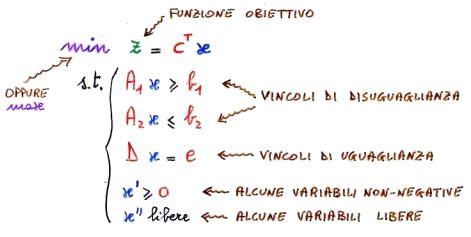
\includegraphics[width=1\columnwidth]{img/ricerca_operativa.jpg}
\end{center}

\vfill
Materia: Ricerca Operativa

Docente: Lorenzo Castelli

%----------------------------------------------
% INDICE
%----------------------------------------------

\clearpage
\tableofcontents

%----------------------------------------------
% INIZIO CAPITOLI
%----------------------------------------------
%CAPITOLO
\clearpage
\section{21/09/2021 - Concetti introduttivi}
\subsection{Ottimizzazione dei problemi}
\subsubsection{Definizione}
Un problema ottimizzato è definito specificando:
\begin{itemize}
\item Un insieme $E$: Elementi che vengono chiamati "soluzione"\\
\item Un sotto insieme $F\subset E$ 
\item Una funzione $f: E \rightarrow \R$ denominata come funzione oggetto che dev'essere minimizzata o massimizzata (a seconda del problema)
\end{itemize}

\subsection{Convessità}
\subsubsection{Definizione}
Una funzione $f(x)$ di una variabile è una funzione convessa se, per ogni coppia $x'$ e $x''$ di valori (con $x'<x''$) si ha $$f[\lambda x'' + (1-\lambda)x'] \leq \lambda f(x'')+(1-\lambda)f(x')$$ per ogni valore di $\lambda$ tale che $0<\lambda <1$\\
\\
\begin{itemize}
\item Una funzione è \textsl{strettamente convessa} se si può sostituire $\leq$ con $<$\\
\item Una funzione è \textsl{concava} se la condizione sopra citata vale quando si sostituisce $\leq$ con $\geq$\\
\item Una funzione è \textsl{strettamente concava} se si può sostituire $\geq$ con $>$\\
\end{itemize}

\subsubsection{Funzione convessa}
\begin{center}
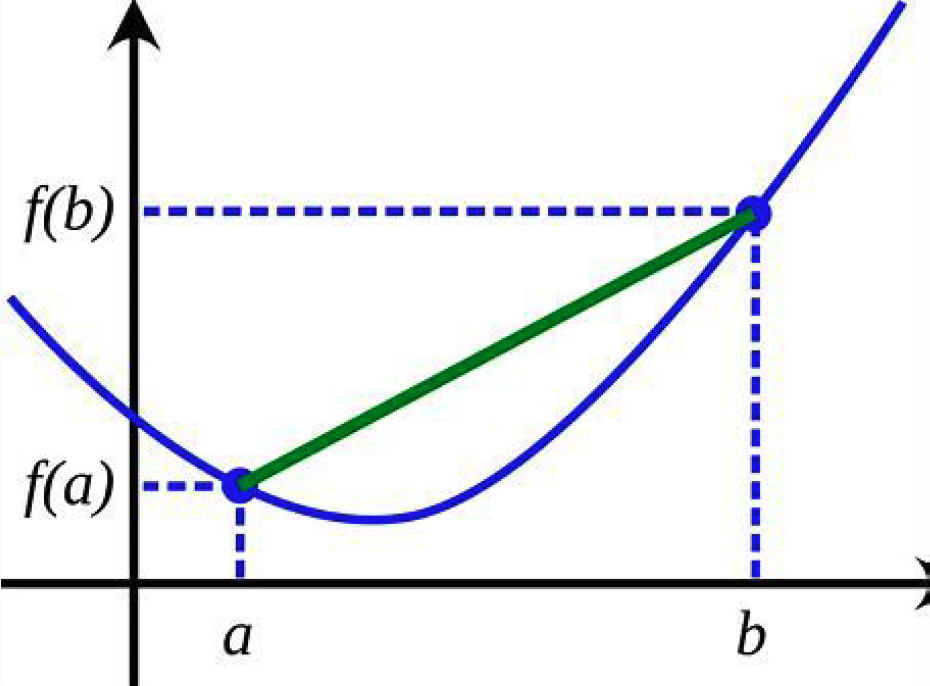
\includegraphics[width=0.3\columnwidth]{img/f_convessa.png}
\end{center}
La funzione $f(x)$ è convessa se per ogni coppia di punti del grafico $f(x)$ il segmento che li congiunge sta interamente al di sopra del grafico di $f(x)$ o coincide con esso.\\
\\
Una funzione strettamente convessa è anche convessa, ma una funzione convessa non è strettamente convessa se la sua derivata seconda è uguale a zero per alcuni valori di $x$.

\subsubsection{Funzione concava}
\begin{center}
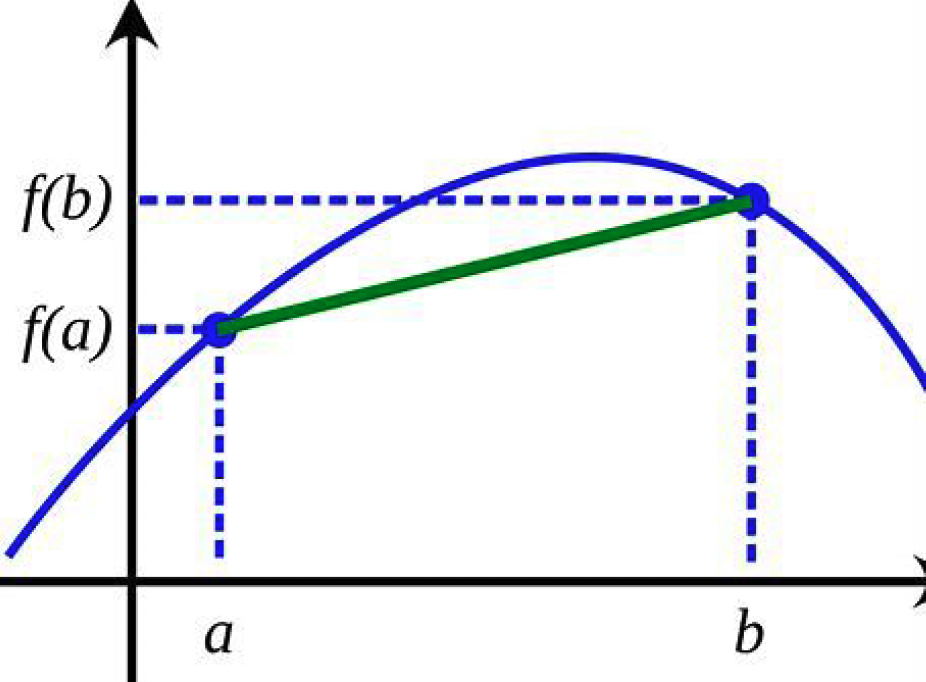
\includegraphics[width=0.3\columnwidth]{img/f_concava.png}
\end{center}
La funzione $f(x)$ è concava se per ogni coppia di punti del grafico $f(x)$ il segmento che li congiunge sta interamente al di sotto del grafico di $f(x)$ o coincide con esso.\\
\\
Una funzione strettamente concava è anche concava, ma una funzione concava non è strettamente concava se la sua derivata seconda è uguale a zero per alcuni valori di $x$.

\subsubsection{Funzione Lineare}
\begin{center}
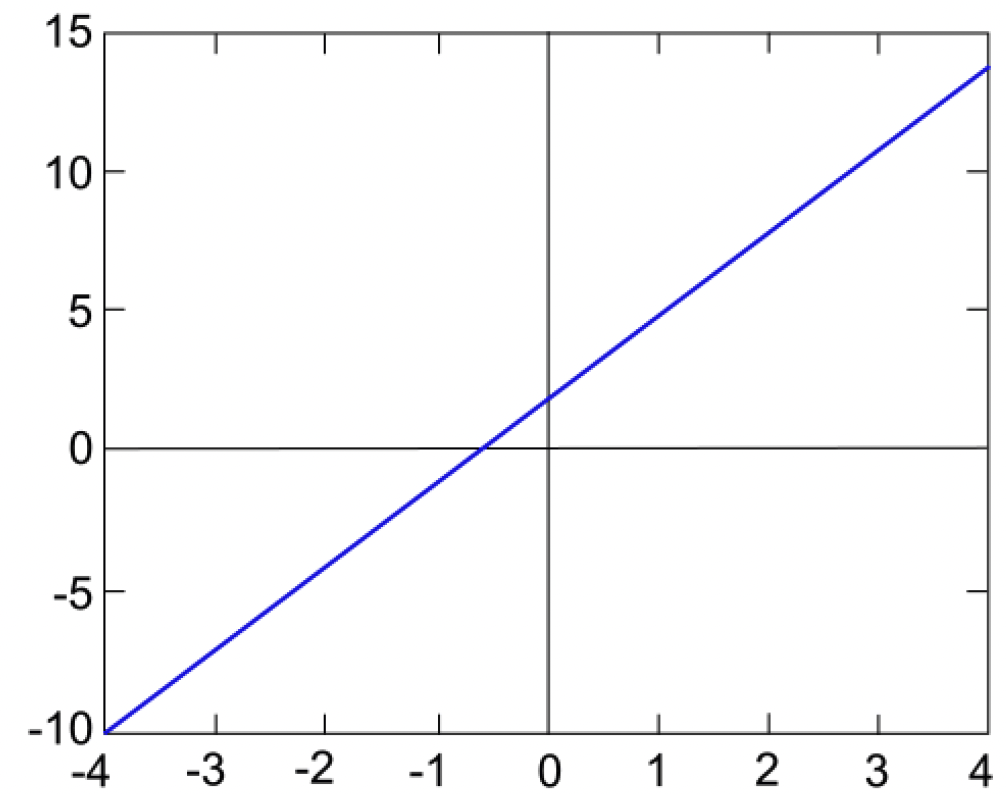
\includegraphics[width=0.3\columnwidth]{img/f_lineare.png}
\end{center}
Una funzione lineare è una funzione che è sia concava che convessa.

\subsubsection{Test di convessità}
Sia $f(x)$ una funzione di una sola variabile che ammette derivata seconda per tutti i possibili valori di $x$. Allora $f(x)$ è:
\begin{itemize}
\item \textsl{Convessa} se e solo se ${d^2f(x) \over dx^2} \geq 0$ per ogni possibile valore di $x$\\
\item \textsl{Strettamente convessa} se e solo se ${d^2f(x) \over dx^2} > 0$ per ogni possibile valore di $x$\\
\item \textsl{Concava} se e solo se ${d^2f(x) \over dx^2} \leq 0$ per ogni possibile valore di $x$\\
\item \textsl{Strettamente concava} se e solo se ${d^2f(x) \over dx^2} < 0$ per ogni possibile valore di $x$\\
\end{itemize}

\subsection{Insiemi convessi}
\subsubsection{Definizione}
Un insieme convesso è un insieme di punti tale che, per ogni coppia di punti dell’insieme, il segmento che li congiunge è interamente contenuto nell’insieme.
\begin{center}
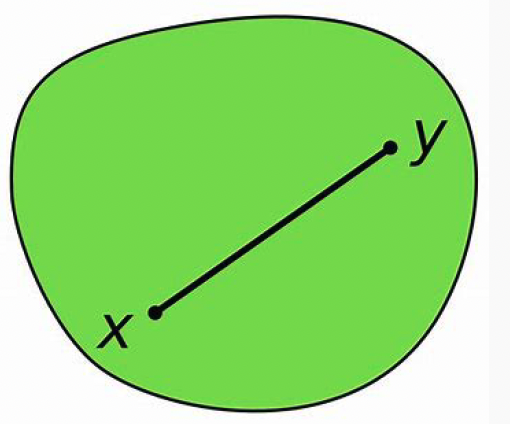
\includegraphics[width=0.3\columnwidth]{img/ins_covesso.png}
\end{center}
\subsubsection{Intersezione di insiemi convessi}
L'intersezione di insiemi convessi è un insieme convesso.

\subsection{Punto estremo}
\subsubsection{Definizione}
Un punto estremo di un insieme convesso è punto dell’insieme che non appartiene ad alcun segmento congiungente altri due punti distinti dell’insieme\\
\begin{center}
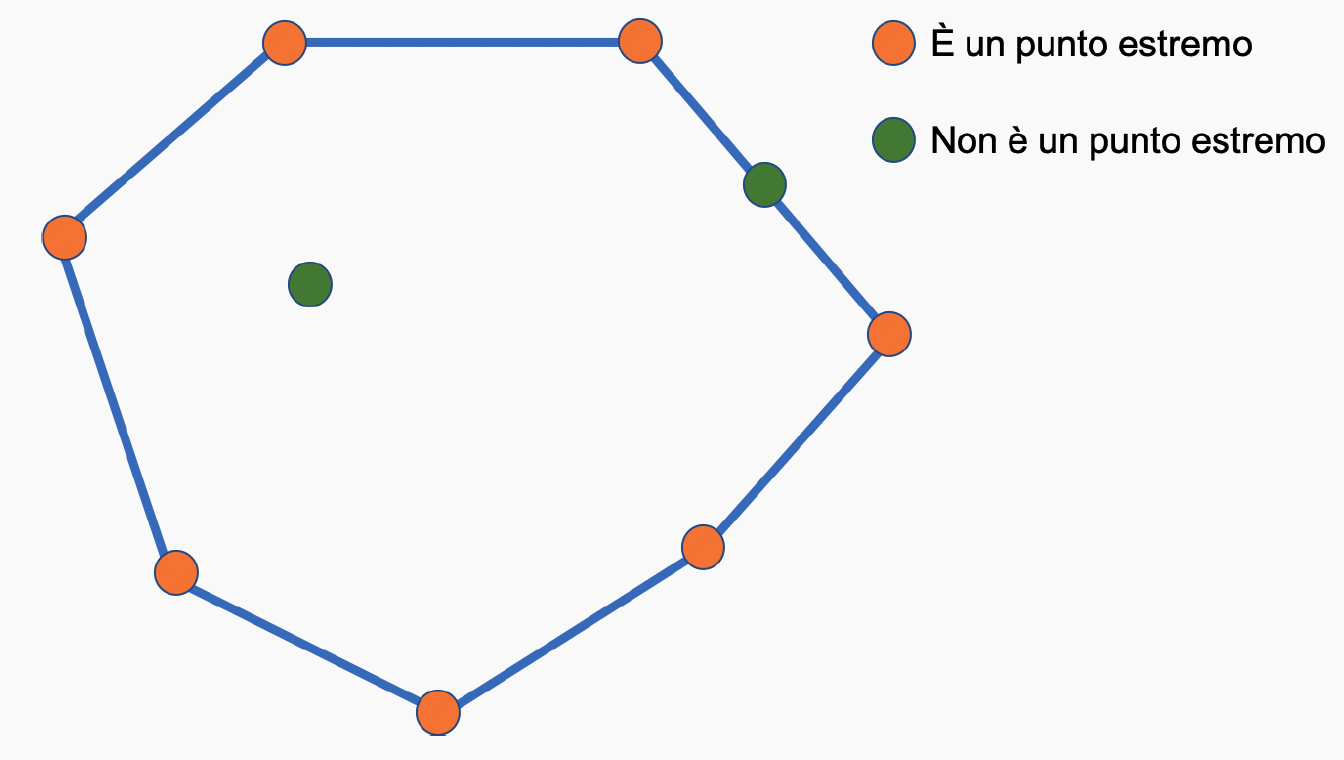
\includegraphics[width=0.3\columnwidth]{img/p_estremo.png}
\end{center}
\textbf{N.B}: Non tutti gli insiemi convessi hanno punti estremi

\subsection{Ottimizzazione non vincolata}
Si consideri una funzione di una sola variabile e derivabile.\\
Condizione necessarie affinché una particolare soluzione $x=x*$ sia un minimo o un massimo è che ${df(x) \over dx} = 0 \ in \ x=x_*$\\
\begin{center}
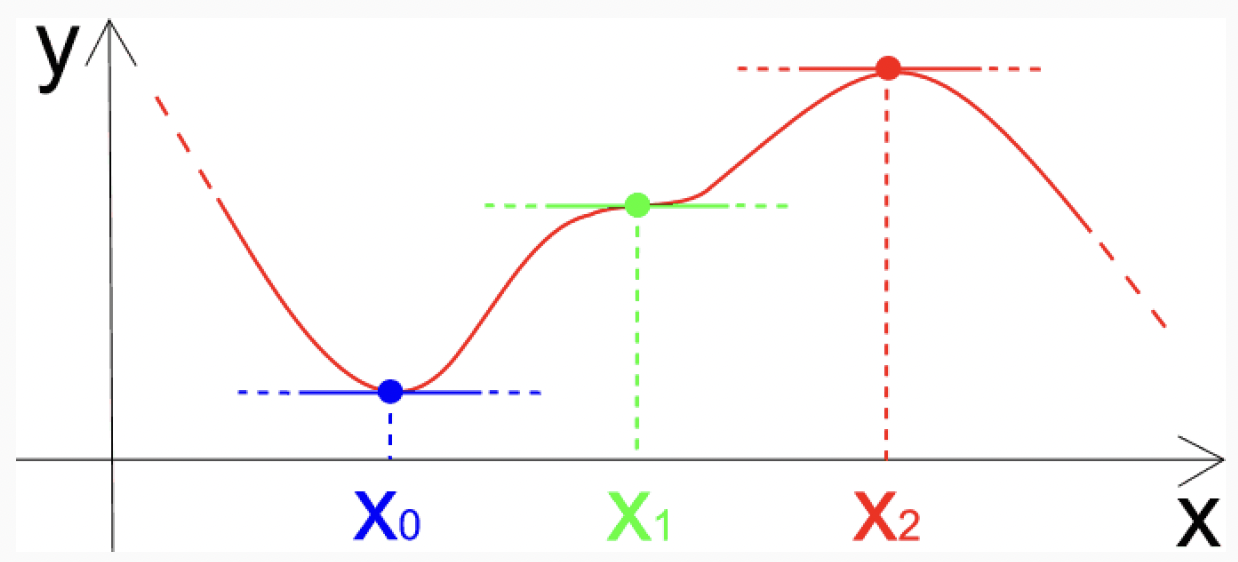
\includegraphics[width=0.3\columnwidth]{img/punti_critici.png}
\end{center}
Per avere maggiori informazioni sui punti critici \textcolor{blue}{$x_0$ (punto di minimo)}, \textcolor{green}{$x_1$ (punto di flesso)} e \textcolor{red}{$x_2$ (punto di massimo)} è necessario esaminare la derivata seconda\\
\\
\textbf{N.B.}: Se la funzione non è derivabile in tutto il dominio la proprietà sopra enunciata non vale

\subsection{Minimi e massimi locali}
Se ${d^2f(x) \over dx^2} > 0 \ in \ x=x*$ allora $x*$è almeno un minimo locale (cioè $f(x*) \leq f(x)$ per ogni $x$ sufficientemente vicino a $x*$. In altre parole, $x*$ è un minimo se $f(x)$ è strettamente convessa in un intorno di $x*$.\\
Analogamente, una condizione sufficiente affinché $x*$ sia un massimo locale (supponendo che soddisfi la condizione necessaria) è che $f(x)$ sia strettamente concava in un intorno di $x*$ (cioè la derivata seconda è negativa in $x*$). Se la derivata seconda è nulla è necessario esaminare le derivate di ordine superiore (in questo caso il punto potrebbe anche essere un punto di flesso).

\subsection{Minimi e massimi globali}
Per determinare un minimo globale (cioè una soluzione $x*$ tale che $f(x*) \leq f(x), \ \forall x$) è necessario confrontare i minimi locali e identificare quello per il quale si ha il più piccolo valore di $f(x)$. Se questo valore è minore di $f(x)$ per $x \rightarrow - \infty$ e per $x \rightarrow + \infty$ (o agli estremi del suo dominio, se essa è definita in un intervallo limitato),
allora questo punto è un minimo globale.\\
Il massimo globale è determinato in modo analogo.

\subsubsection{Minimi globali per funzioni convesse}
Se $f(x)$ è una funzione convessa, allora una qualunque soluzione $x*$ tale che ${df(x) \over dx} = 0 \ in \ x=x*$ è automaticamente un minimo globale. In altre parole questa condizione è non solo necessaria ma anche sufficiente per un minimo globale di una funzione convessa. Questa soluzione non deve necessariamente essere unica perché la funzione potrebbe rimanere costante in un certo intervallo nel quale la sua derivata è nulla.\\
D’altra parte se $f(x)$ è strettamente convessa allora questa soluzione deve essere l’unico minimo globale.

\subsubsection{Massimi globali per funzioni concave}
Analogamente se $f(x)$ è una funzione concava, allora la condizione ${df(x) \over dx} = 0 \ in \ x=x*$ è sia necessaria che sufficiente affinché $x*$ sia un massimo globale.\\
\\
Se la funzione non è strettamente concava o strettamente convessa ci possono essere infinite soluzioni ottime, rispettivamente massimi e minimi globali.

%CAPITOLO
\clearpage
\section{23/09/2021 - Esempi di modelli}
\subsection{La compilation ideale - Problema dello zaino}
Si vuole realizzare una compilation ideale avendo disposizione dei file musicali e un CD-ROM dalla capacità di 800 MB. l’indice di gradimento (in una scala da 1 a 10) e l’ingombro in MB di ogni file sono riportati nella tabella seguente.\\
\begin{center}
\begin{tabular}{|c|c|c|}
\hline
Canzone & Gradimento & Ingombro\\
\hline
Light my fire & 8 & 210\\
Fame & 7 &190\\
I will survive & 8,5 & 235\\
Imagine &9 &250\\
Let it be &7,5& 200\\
I feel good &8 &220\\
\hline
\end{tabular}
\end{center}
Si vuole decidere quali file inserire nel CD in modo tale da massimizzare il gradimento complessivo senza eccedere la capacità del CD.\\
\\
\paragraph{Formulazione}: Il problema può essere modellato per mezzo di variabili decisionali binarie associate a ogni file musicale in modo tale che assumono valore uno se il file in questione e inserito nel CD valore zero in caso contrario.
Indicato con $g_i$ il gradimento della canzone $i$-esima, con $w_i$ il suo ingombro e con $C$ la capacità del CD il problema può essere formulato per mezzo del seguente problema PLI:
$$\begin{array}{cl}
max \ z = & \sum_{i=1}^n g_ix_i\\
& \sum_{i=1}^n w_ix_i \leq C\\
& x_i \in \{0,1\} \ \ \forall i = 1, \dots, n
\end{array}$$
dove $n = 6$ è il numero di file musicali. L’unico vincolo del problema consiste nel fatto che l’ingombro dei file inseriti non deve eccedere la capacità del CD.\\
\\
\textbf{Soluzione del problema}: \href{https://units.enricolacchin.com/ricop21/problema_dello_zaino.xlsx}{EXCEL}

\subsection{I treni combinati}
Una compagnia ferroviaria deve decidere quanti treni combinati realizzare potendo scegliere tra due diversi modelli DeLuxe e FarWest. La composizione dei due treni è schematizzata nella tabella seguente.\\
\begin{center}
\begin{tabular}{|c|c|c|c|}
\hline
Tipo di Vagone & DeLuxe & Far West & Disponibilità\\
\hline
Merci & 1 & 3 & 12\\
WLit & 1 &0 & 9\\
Ristorante & 1 & 0 & 10\\
II Classe &2 &3 & 21\\
I Classe &1& 2 & 10\\
Motrice &1 &1 & 9\\
\hline
Guadagno & 3000€ & 8000€ & \\
\hline
\end{tabular}
\end{center}
Si vuole massimizzare il guadagno totale\\
\\
Poiché dobbiamo decidere quanti treni di ciascun tipo realizzare il problema può essere formulato per mezzo di due variabili
decisionali $x_1$ e $x_2$ che rappresentano rispettivamente il numero di treni Deluxe e il numero di treni Far West da realizzare: ovviamente tali variabili dovranno risultare intere e non negative.\\
$$\begin{array}{cl}
max \ z = & 3x_1+8x_2\\
& x_1+2x_2 \leq 10\\
& 2x_1+3x_2 \leq 21\\
& x_1+3x_2 \leq 12\\
& x_1 \leq 9\\
& x_1 \leq 10\\
& x_1 + x_2 \leq 9\\
& x_1,x_2 \geq 0, \ interi\\
\end{array}$$
\noindent
\textbf{Soluzione del problema}: \href{https://units.enricolacchin.com/ricop21/treni_combinati.xlsx}{EXCEL} - \href{https://units.enricolacchin.com/ricop21/treni_combinati.xlsx}{PDF}

%CAPITOLO
\clearpage
\section{27/09/2021 - Introduzione alla programmazione lineare}
\subsection{Problema di programmazione lineare}
Un problema di programmazione lineare (LP) è un'ottimizzazione di un problema tale che
$$z=max\{c(x):x\in X \subseteq \R^n\}$$
oppure 
$$z=min\{c(x):x\in X \subseteq \R^n\}$$
dove \begin{itemize}
\item La funzione obiettivo $c(x): \R^n \rightarrow \R$ è lineare. Perciò $c(x)=cx$ dove $c$ è un vettore in $\R^n$
\item L'insieme $X$ delle soluzioni ammissibili è definito da vincoli lineari tali che $h(x)=\gamma$ e/o $h(x) \leq \gamma$, dove $h(x): \R^n \rightarrow \R$ è una funzione linare e $\gamma$ uno scalare in $\R$
\end{itemize}

\subsubsection{Formulazione}
Un problema di programmazione lineare può essere formulato come
$$\begin{array}{rl}
max\ z & = c^Tx\\
& Ax \leq b\\
& x \geq 0
\end{array}$$
oppure
$$\begin{array}{rl}
max\ Z & = c_1x_1 + c_2x_2 +\dots + c_nx_n\\
& a_{11}x_1 + a_{12}x_2 + \dots + a_{1n}x_n \leq b_1\\
& a_{21}x_1 + a_{22}x_2 + \dots + a_{2n}x_n \leq b_2\\
& \vdots\\
& a_{m1}x_1 + a_{m2}x_2 + \dots + a_{mn}x_n \leq b_m\\
& x_1,x_2,\dots, x_n \geq 0
\end{array}$$
\textbf{Notazione}:\begin{itemize}
\item $m$: numero di righe della matrice $A$
\item $n$: dimensione del vettore $x$ e numero di colonne della matrice $A$
\item $c$: vettore della funzione obiettivo
\item $A$: matrice
\item $b$: vettore dei termini noti
\item $x$: vettore delle variabili decisionali
\item $X=\{x:Ax\leq b, x \geq 0\}$: insieme delle soluzioni ammissibili.
\end{itemize}

\subsubsection{Proprietà}
\paragraph{Proporzionalità}: La funzione obiettivo e ogni vincolo devono essere lineari con
rispetto a ciascuna variabile decisionale. In altre parole, la misura dell'efficacia e l'uso della risorsa devono essere proporzionati al livello di ogni attività svolta individualmente, cioè se $x_j \not =0$ e $x_1=x_2=\dots=x_{j-1}=x_{j+1}=\dots=x_n = 0$ deve essere $Z=c_jx_j$ e $a_{ij}x_j \leq b_i, \ \forall i, \forall j$\\
Pertanto devono sempre valere le seguenti proprietà:
$${\partial Z \over \partial x_j} =c_j \ \forall j \ \ \ \ \ {\partial b_i \over \partial x_j}\geq a_{ij} \ \forall i \forall j$$
cioè, la misura marginale dell'efficacia e l'uso marginale di ciascuna risorsa deve essere costante su tutto il range di variazione dei livelli di ciascuna attività.

\paragraph{Fixed Charge}: Un caso in cui non è possibile applicare il LP è quando abbiamo una tariffa fissa. Questo accade ogni volta che c'è una tariffa di preparazione o un costo di installazione associato a un'attività.\\
Cioè, se $x$ è il livello di una certa attività e la funzione obiettivo è
\begin{equation*}
f(x) = \begin{cases} \begin{array}{ll}0 & x=0\\K+cx & x > 0\end{array}\end{cases}
\end{equation*}
La proprietà di proporzionalità è violata.

\paragraph{Addittività}: Non devono esserci interazioni tra le varie attività, cioè la misura totale dell'efficacia derivata dal risultato congiunto delle attività deve essere pari alla somma delle quantità risultanti da ogni attività svolta individualmente.\\
In pratica, se $c_1x_1,c_2x_2, \dots , c_nx_n$ è la misura dell'efficacia per le attività $1,2,\dots, n$ condotte individualmente, deve succedere che $Z=c_1x_1+c_2x_2+\dots+c_nx_n$ (dove $Z$ è la misura totale dell'efficacia).\\
Analogamente vale per l'utilizzo totale delle risorse.

\paragraph{Divisibilità (o Continuità)}: Il valore di $x_j$ sono numeri reali $\rightarrow x\in \R^n$\\
Va notato che questo non ha sempre senso, cioè, a volte la soluzione che stiamo cercando deve essere intera. Però, in tal caso, se la regione ammissibile non è vuota, possiamo sempre trovare un vettore $x$ che rispetta i vincoli anche senza essere intero.\\
Escludiamo sempre il caso di valori complessi.

\paragraph{Certezza}: Tutti i coefficienti del problema sono numeri reali costanti noti a priori. Non c'è niente di stocastico, niente di casuale.

\subsection{Possibili uscite di un problema LP}
\begin{center}
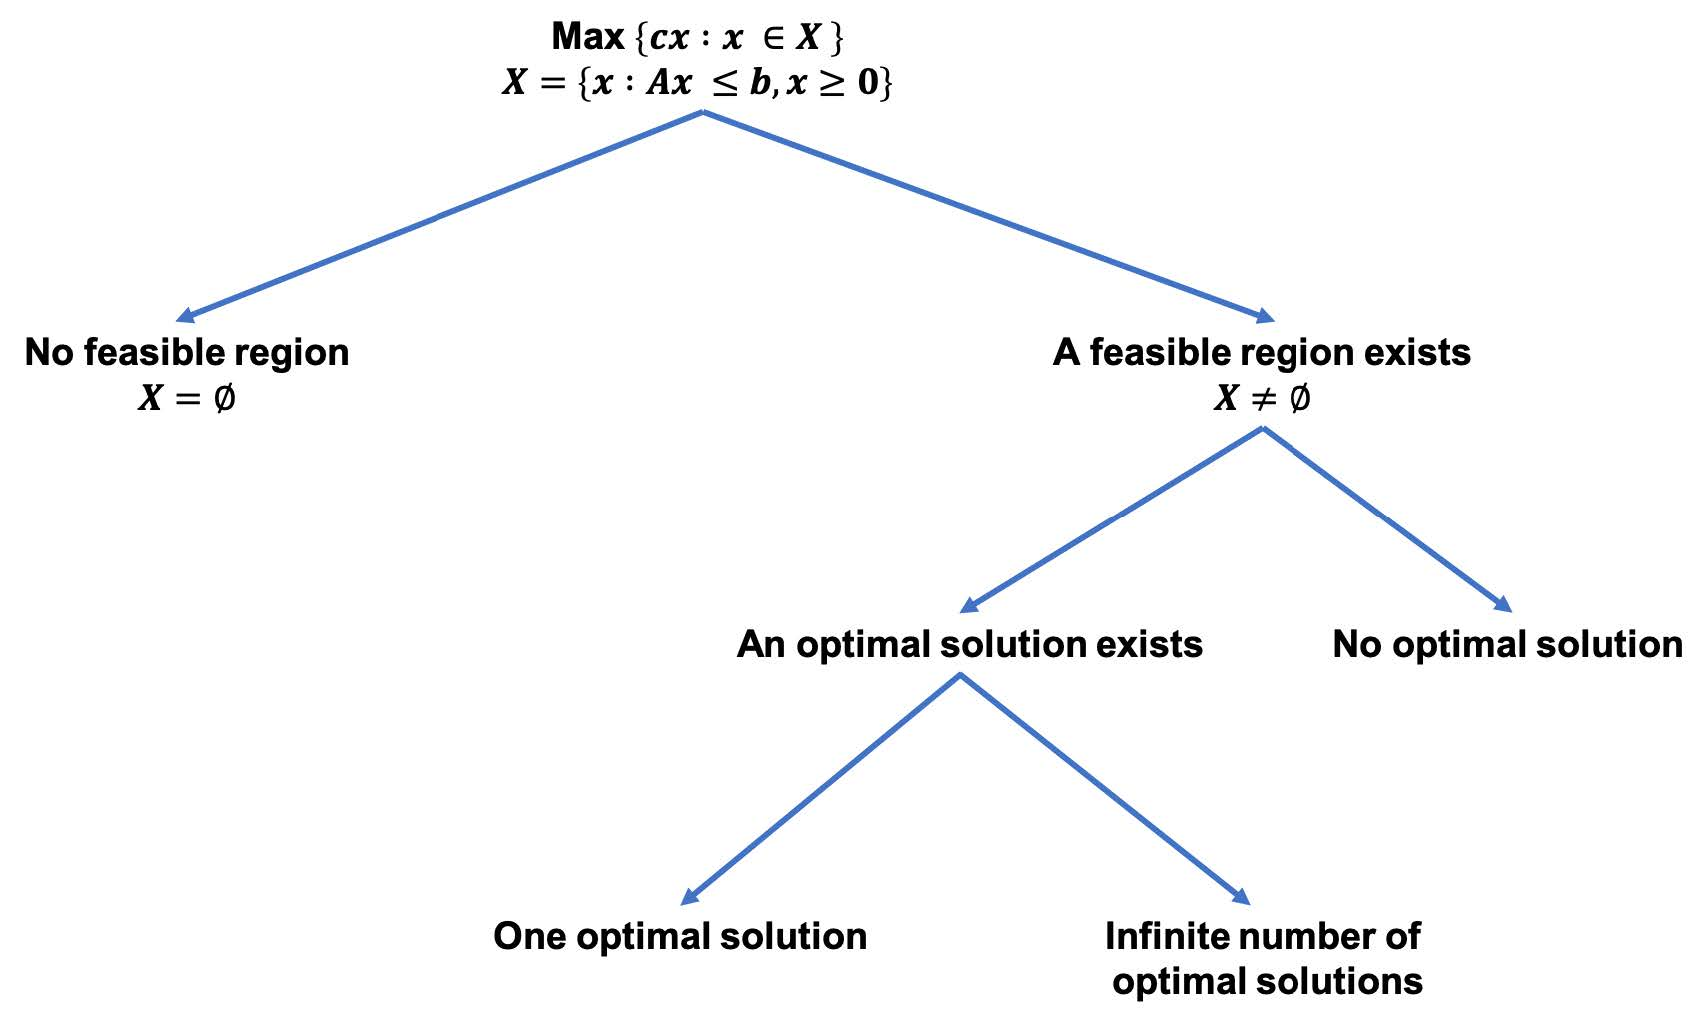
\includegraphics[width=0.8\columnwidth]{img/lp_solutions.jpg}
\end{center}
\subsubsection{Nessuna regione ammissibile}
\begin{center}
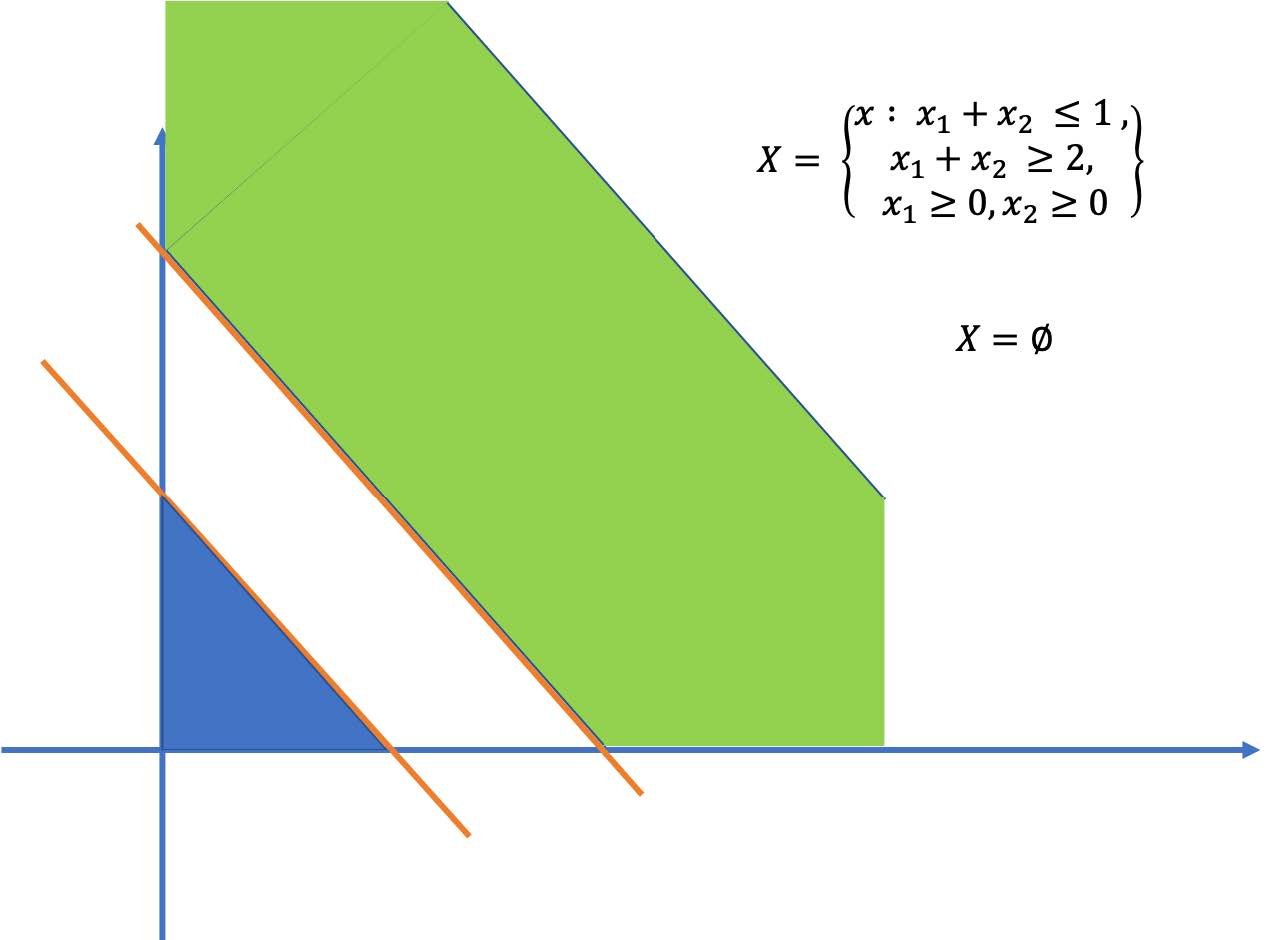
\includegraphics[width=0.4\columnwidth]{img/no_region.jpg}
\end{center}
\subsubsection{Nessuna soluzione ottima}
\begin{center}
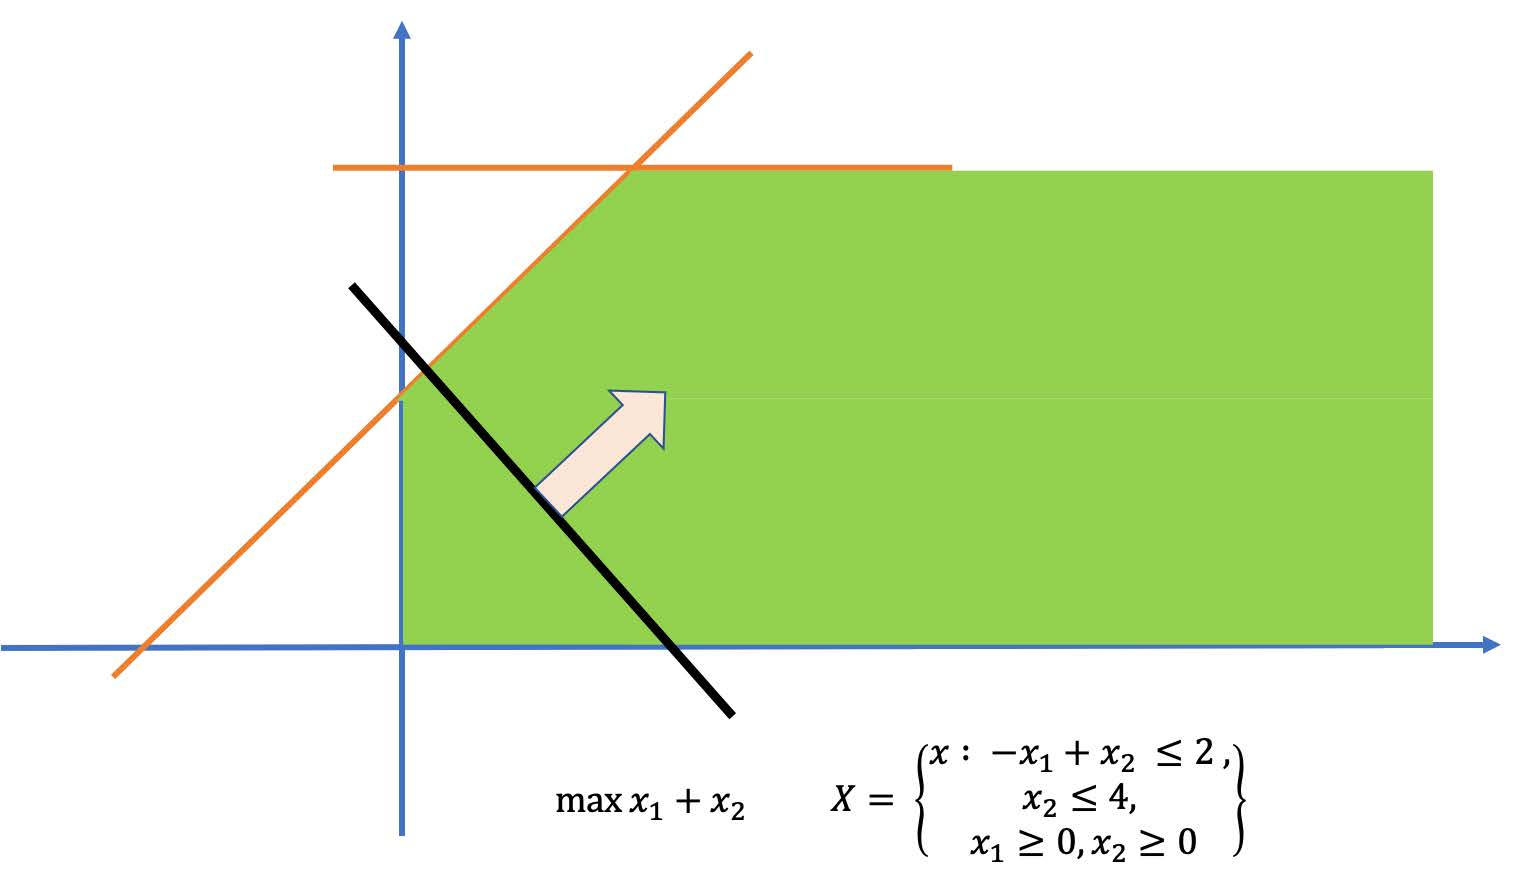
\includegraphics[width=0.4\columnwidth]{img/no_sol.jpg}
\end{center}
\subsubsection{Soluzione ottima}
\begin{center}
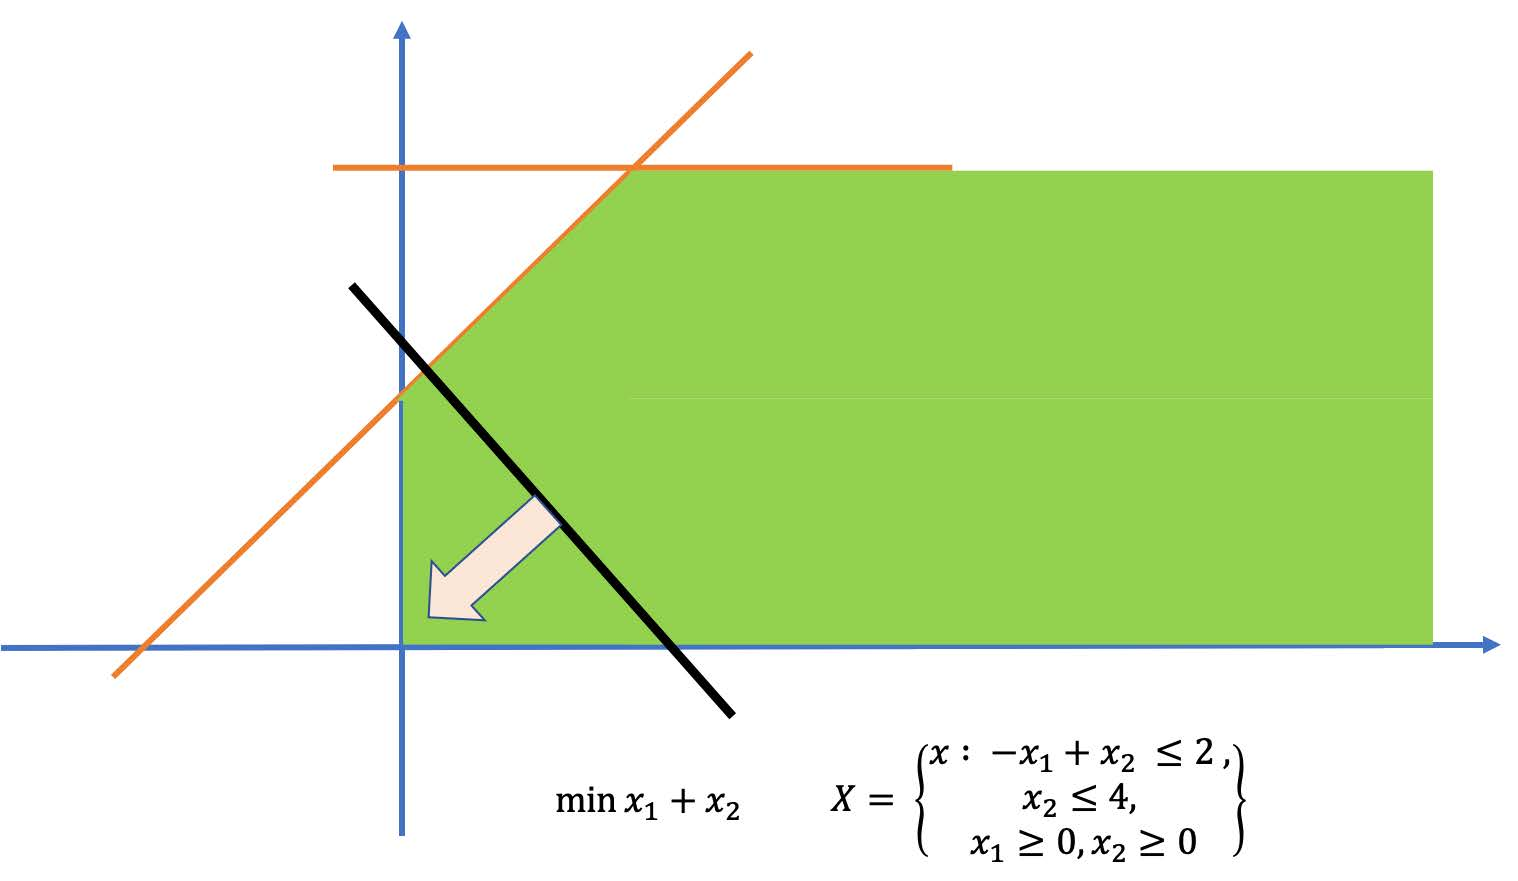
\includegraphics[width=0.4\columnwidth]{img/opt_sol.jpg}
\end{center}
\subsubsection{Unica soluzione ottima}
\begin{center}
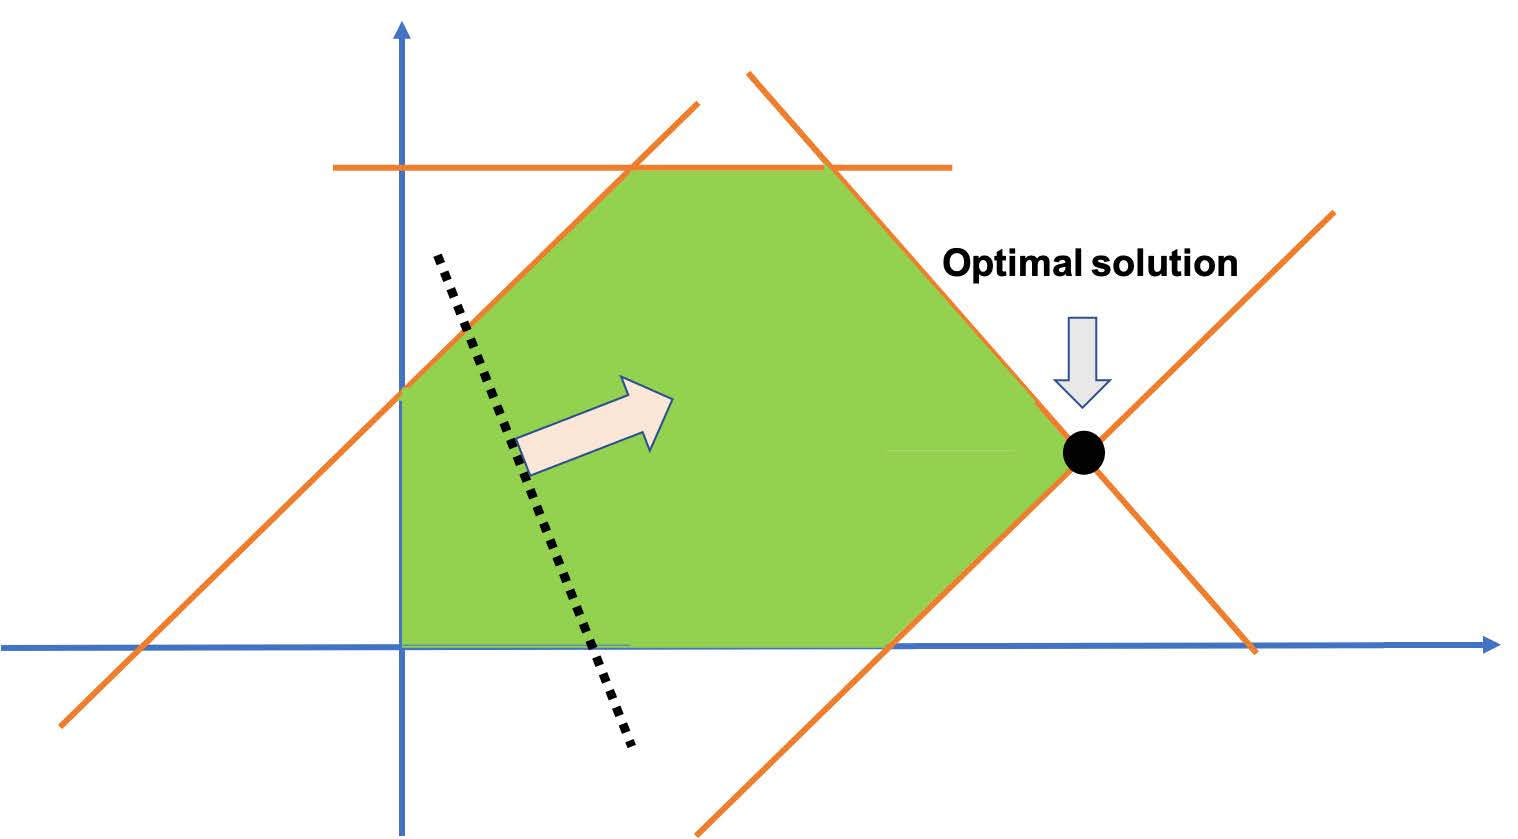
\includegraphics[width=0.4\columnwidth]{img/one_opt_sol.jpg}
\end{center}
\subsubsection{Infinite soluzioni ottime}
\begin{center}
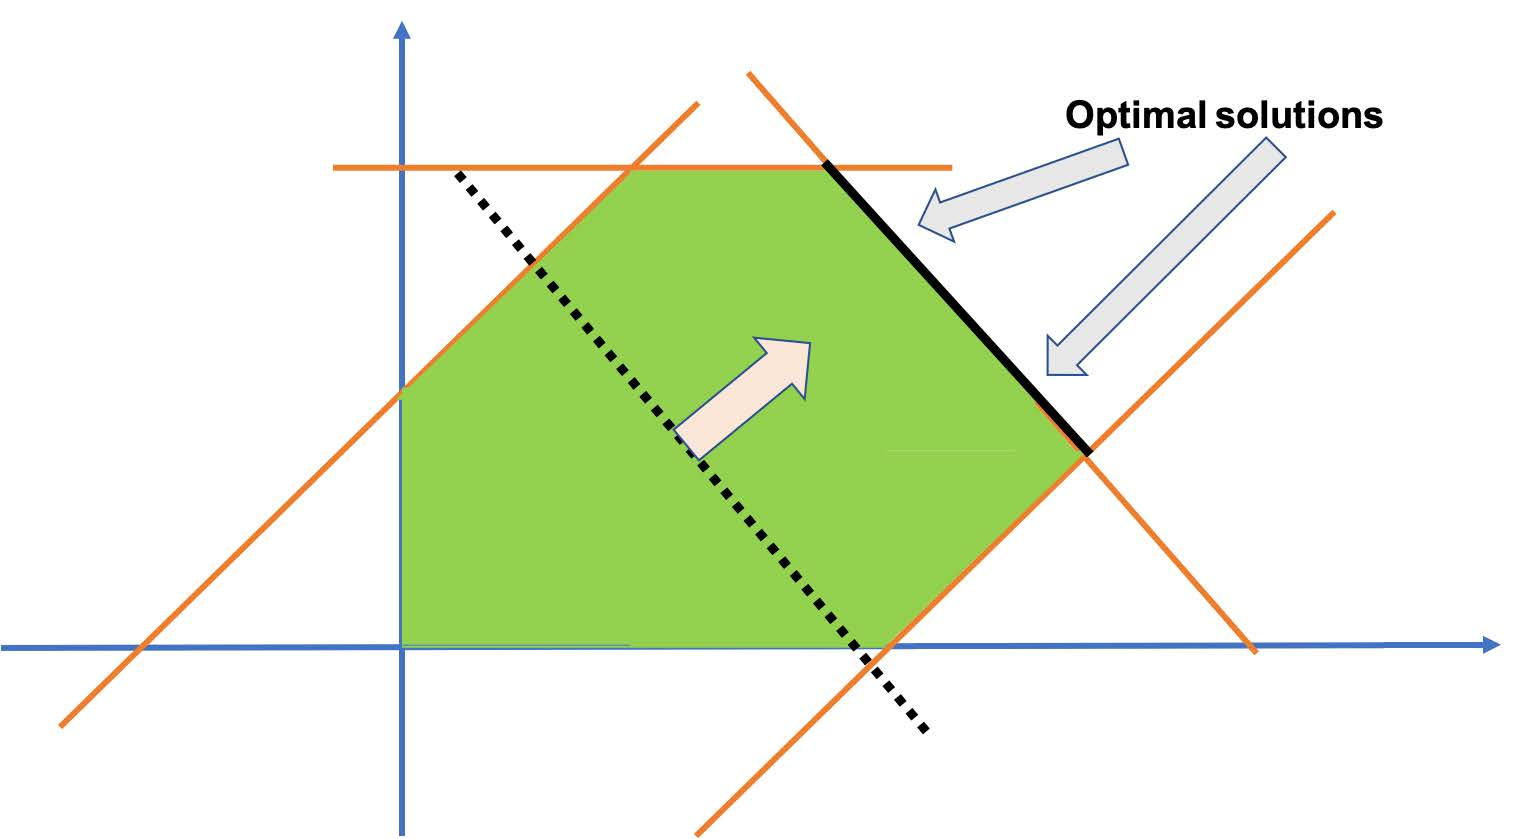
\includegraphics[width=0.4\columnwidth]{img/inf_opt_sol.jpg}
\end{center}

\subsection{Definizioni}
\paragraph{Iperpiano}: Chiamiamo iperpiano l'insieme $H=\{x\in\R^n:a^Tx=b\}$ dove $a\in \R^n, a\not = 0, b\in \R$. Le regioni $X^- =\{x\in \R^n:a^Tx \leq b\}$ e $X^+=\{x\in \R^n:a^Tx \geq b\}$ sono detti semispazi delimitati dal supporto dell'iperpiano $H$.

\paragraph{Poliedro}: Chiamiamo poliedro (convesso) l'intersezione di un numero finito di semispazi e iperpiani.

\paragraph{Politopo}: Chiamiamo politopo un poliedro limitato $P$, cioè esiste una costante $M>0$ tale che $\|x\| \leq M \ \ \forall x \in P$

\paragraph{Lemma}: La regione ammissibile di un problema LP è un poliedro convesso.

\paragraph{Vertice}: I punti estremi di un polierdo convesso.

\subsection{Teorema chiave}
Dato un problema lineare $$\begin{array}{rl}
max\ z & = cx\\
& Ax = b \ \ (b\geq 0)\\
& x \geq 0
\end{array}$$
Se $X\not = \emptyset$ e ha una soluzione ottima e finita, allora esiste un vertice di $X$ che è una soluzione ottima.\\
La dimostrazione si basa sul fatto che $X$ è un poliedro e quindi è un insieme convesso.

%CAPITOLO
\clearpage
\section{30/09/2021 - L'algoritmo del simplesso (fondamenti)}
\subsection{Soluzione d'angolo}
\begin{center}
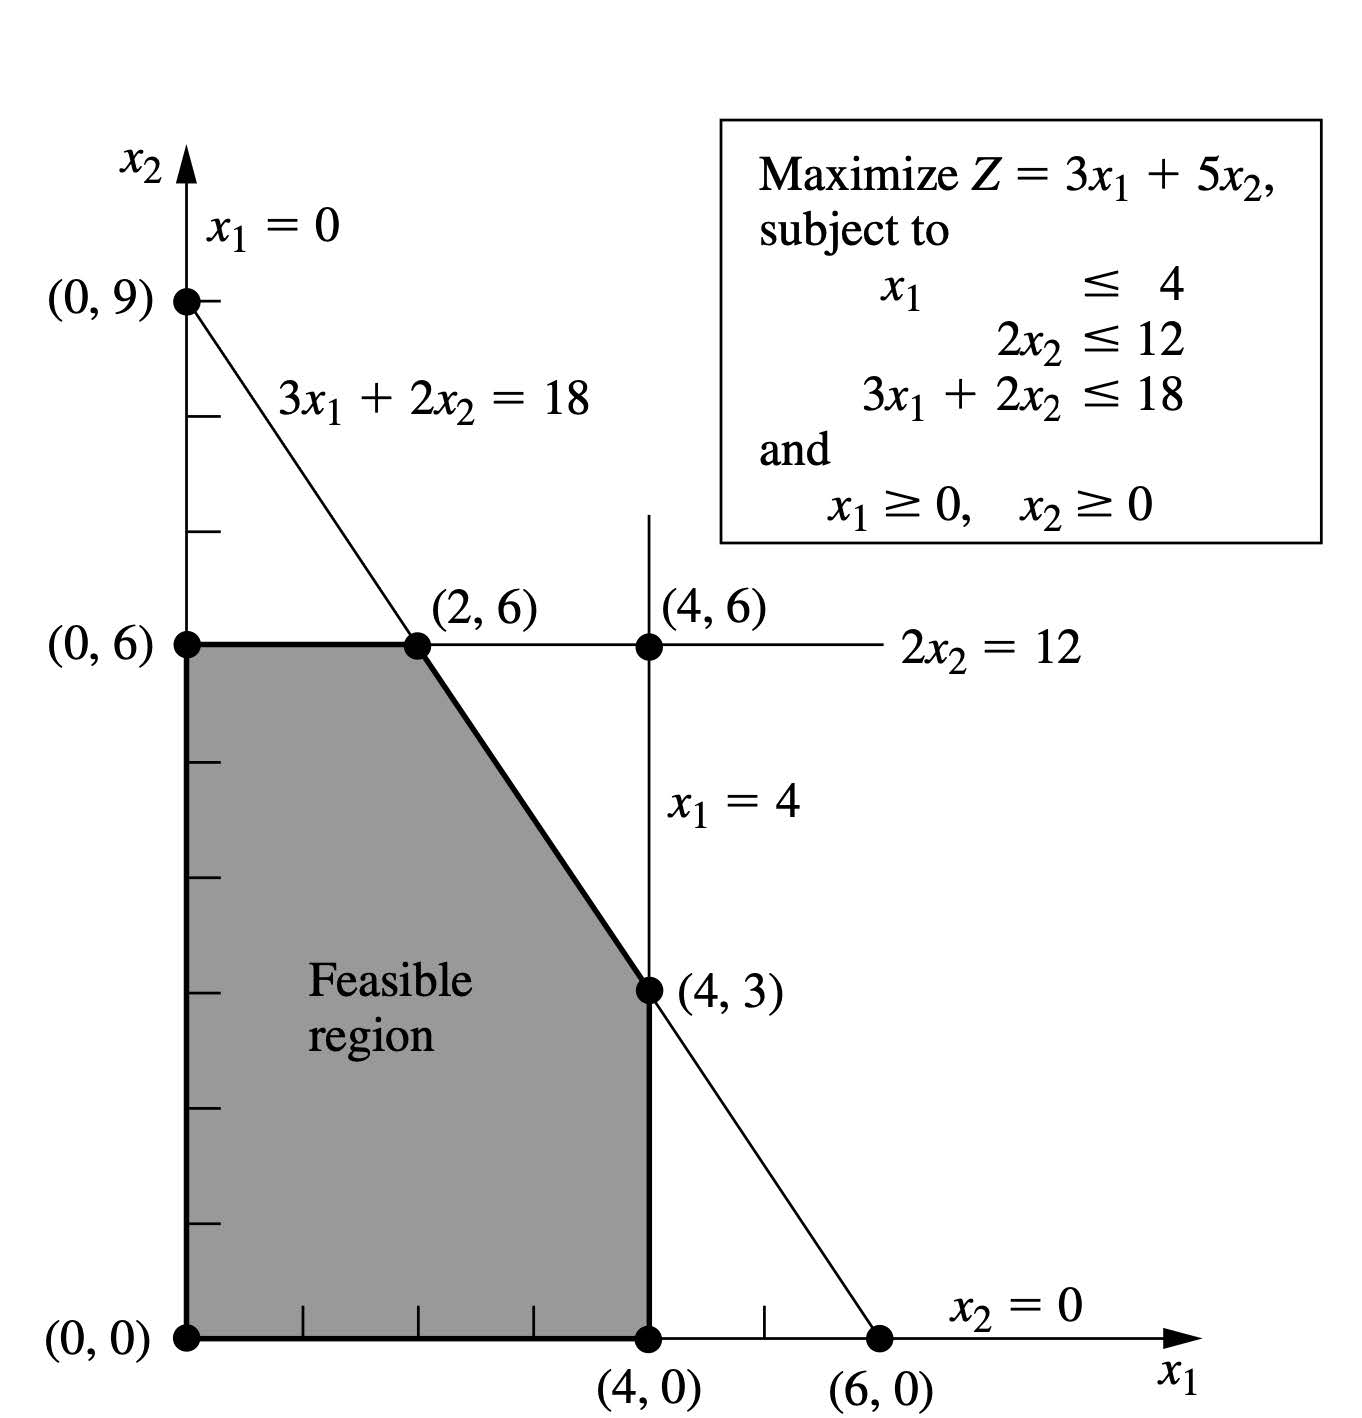
\includegraphics[width=0.4\columnwidth]{img/es210927.jpg}
\end{center}
Un confine di vincolo è una linea che forma il confine di ciò che è consentito dal vincolo corrispondente.\\
I punti di intersezione sono le soluzioni dei vertici del problema. I cinque che si trovano agli angoli della regione ammissibile - $(0, 0), (0, 6), (2, 6), (4, 3)$ e $(4, 0)$ - sono le soluzioni ammissibili ai vertici (soluzioni CPF). Le altre tre - $(0, 9), (4, 6)$ e $(6, 0)$ - sono chiamate
soluzioni irrealizzabili.\\
In questo esempio, ogni soluzione del punto d'angolo si trova all'intersezione di due limiti di vincolo. Per un problema LP con $n$ variabili decisionali, ciascuna delle sue soluzioni del punto d'angolo si trovano all'intersezione di $n$ limiti di vincolo.

\subsection{Soluzioni CPF adiacenti}
Alcune coppie delle soluzioni CPF nell'esempio condividono un vincolo confine, e altre coppie no. Sarà importante distinguere tra questi casi utilizzando le seguenti definizioni generali.\\
\textcolor{blue}{\textbf{Definizione}:} Per qualsiasi problema LP con $n$ variabili decisionali, due soluzioni CPF sono adiacenti tra loro se condividono $n-1$ limiti di vincolo. Le due soluzioni CPF adiacenti sono collegate da un segmento di linea che giace su questi stessi confini di vincoli condivisi. Tale segmento di linea è detto bordo (spigolo) della regione ammissibile.\\
Poiché $n = 2$ nell'esempio, due delle sue soluzioni CPF sono adiacenti se ne condividono un limite di vincolo; per esempio, $(0, 0)$ e $(0, 6)$ sono adiacenti perché condividono il limite di vincolo $x_1 = 0$ . La regione ammissibile ha cinque bordi, costituiti da i cinque segmenti di linea che formano il confine di questa regione. Nota che due bordi emanano da ciascuna soluzione CPF. Quindi, ogni soluzione CPF ha due soluzioni CPF adiacenti (ciascuna giacente all'altra estremità di uno dei due bordi), come enumerato di seguito
\begin{center}
\begin{tabular}{c|c}
Soluzione CPF & Soluzione CPF adiacente\\\hline
$(0,0)$ & $(0,6)$ e $(4,0)$\\
$(0,6)$ & $(2,6)$ e $(0,0)$\\
$(2,6)$ & $(4,3)$ e $(0,6)$\\
$(4,3)$ & $(2,6)$ e $(4,0)$\\
$(4,0)$ & $(0,0)$ e $(4,3)$\\
\end{tabular}
\end{center}

\subsection{Proprietà 1 - La soluzione ottima è su un vertice}
\begin{enumerate}
\item Se esiste esattamente una soluzione ottima, allora deve essere una soluzione CPF.
\item Se ci sono più soluzioni ottime (e una regione ammissibile limitata), allora almeno due devono essere soluzioni CPF adiacenti
\end{enumerate}
\textbf{Dimostrazione (1)}: Per assurdo, assumendo che esista esattamente una soluzione ottima e che non sia una soluzione CPF.\\
Ricordiamo la definizione di soluzione CPF (una soluzione ammissibile che non giace su nessun segmento di linea che collega altre due soluzioni ammissibili). Poiché abbiamo assunto che la soluzione ottima $x$ non è una soluzione CPF, questo implica che devono esserci altre due soluzioni fattibili come che il segmento di linea che li collega contenga la soluzione ottima. Facciamo che i vettori $x'$ e $x''$ denotino queste altre due soluzioni ammissibili e indichiamo con $Z_1$ e $Z_2$ il loro rispettivo valore della funzione obiettivo. Come ogni altro punto sul segmento di linea che collega 
$$x^*=\alpha x''+(1-\alpha)x'$$
Per qualche valore di $\alpha$ tale che $0<\alpha < 1$ otteniamo
$$Z^*=\alpha Z_2 + (1-\alpha) Z_1$$
Poiché i pesi $\alpha$ e $1-\alpha$ si sommano a $1$, le uniche possibilità di come $Z^*$, $Z_1$ e $Z_2$ vengono confrontate sono:
\begin{itemize}
\item $Z^* = Z_1 = Z_2$
\item $Z_1 < Z^* < Z_2$
\item $Z_1 > Z^* > Z_2$
\end{itemize}
La prima possibilità implica che $x'$ e $x''$ siano anche loro soluzione ottima che contraddice l'ipotesi che esiste esattamente una soluzione ottima. Entrambe le ultime possibilità contraddicono l'assunto che $x^*$ (non una soluzione CPF) è ottima. La conclusione che ne risulta è che è impossibile avere un singola soluzione ottima che non è una soluzione CPF.\\
\\
\textbf{Dimostrazione (2)}: Quello che succede quando risolvi graficamente è che il la linea della funzione obiettivo continua a sollevarsi finché non contiene il segmento di linea collegando le due soluzioni CPF.\\
La stessa cosa accadrebbe in dimensioni superiori tranne che l'iperpiano della funzione obiettivo continuerebbe a sollevarsi fino a contenere il segmento/i che collega due (o più) soluzioni CPF adiacenti.\\
Di conseguenza, tutte le soluzioni ottime possono essere ottenute come medie ponderate delle soluzioni CPF ottimali.\\

\subsection{Proprietà 2 - Un numero finito di vertici}
C'è solo un numero finito di soluzioni CPF.\\
\textbf{Dimostrazione}: Ogni soluzione CPF è la soluzione simultanea di un sistema di $n$ equazioni con $m + n$ equazioni di confine. Il numero delle diverse combinazioni delle equazioni $m + n$ prese $n$ alla volta è
$$\left(\begin{array}{c}m+n\\n\end{array}\right)={(m+n)!\over m!n!}$$ che è un numero finito.\\
L'enumerazione esauriente potrebbe non essere possibile: un problema di programmazione lineare piuttosto piccolo con solo $m = 50$ e $n = 50$ avrebbero ${100! \over (50!)2}\simeq 10^{29}$ sistemi di equazioni da risolvere!\\
Al contrario, il metodo del simplesso dovrebbe esaminare solo circa $100$ soluzioni CPF per
un problema di queste dimensioni.

\subsection{Proprietà 3 - La regione ammissibile è convessa}
Se una soluzione CPF non ha soluzioni CPF adiacenti che sono migliori (come misurato
da $Z$), allora non ci sono soluzioni CPF migliori da nessuna parte. Pertanto, una tale soluzione CPF è garantita come una soluzione ottima (dalla Proprietà 1), assumendo
solo che il problema possiede almeno una soluzione ottima (garantita se il problema possiede soluzioni ammissibili e una regione ammissibile limitata).

\subsection{Test di ottimalità}
Considera qualsiasi problema di programmazione lineare che ne possieda almeno una soluzione ottima. Se una soluzione CPF non ha soluzioni CPF adiacenti che sono meglio (come misurato da $Z$), allora deve essere una soluzione ottima.\\
\\
Quindi, nell'esempio, $(2, 6)$ deve essere ottimo semplicemente perché il suo $Z = 36$ è
maggiore di $Z = 30$ per $(0, 6)$ e $Z = 27$ per $(4, 3)$. Questo test di ottimalità è il quello utilizzato dal metodo del simplesso per determinare quando una soluzione ottima è stata raggiunta.

\subsection{L'algoritmo del simplesso}
\begin{itemize}
\item \textbf{Inizializzazione}: Sceglie $(0,0)$ come soluzione CPF iniziale da esaminare (Questo è conveniente perché non necessita calcoli per determinare la soluzione CPF)
\item \textbf{Test di ottimalità}: Conclude che $(0,0)$ non è la soluzione ottima (soluzioni CPF adiacenti sono migliori)
\item \textbf{Prima iterazione}: Si muove su una soluzione CPF migliore, $(0,6)$ seguendo tre steps:
\begin{enumerate}
\item Considerando i due bordi della regione ammissibile che emanano da $(0, 0)$, sceglie di muoversi lungo il bordo che porta verso l'alto l'asse $x_2$. (con una funzione obiettivo di $Z = 3x_1 + 5x_2$, salendo l'asse $x_2$ aumenta Z a una velocità maggiore rispetto allo spostamento lungo l'asse $x_1$).
\item Si ferma al primo nuovo limite di vincolo: $2x_2 = 12$. (spostandosi più avanti nella direzione scelta nella fase 1 lascia la regione ammissibile; ad es. muoversi verso il secondo vincolo gli fa colpire il punto $(0, 9)$, che è una soluzione irrealizzabile).
\item Risolve per l'intersezione dei primi due vincoli che incontra: $(0, 6)$. (le equazioni per questi limiti di vincolo, $x_1 = 0$ e $2x_2 = 12$, producono immediatamente questa soluzione).
\end{enumerate}
\item \textbf{Test di ottimalità}: Conclude che $(0,6)$ non è la soluzione ottima (una soluzione CPF adiacenti è migliore)
\item \textbf{Seconda iterazione}: Si muove su una soluzione CPF migliore, $(2,6)$ seguendo tre steps:
\begin{enumerate}
\item Considerando i due bordi della regione ammissibile che emanano da $(0, 6)$, sceglie di muoversi lungo il bordo che porta verso destra (muovendosi in questa direzione incrementa $Z$, mentre se si volesse tornare indietro lungo l'asse $x_2$ la funzione $Z$ diminuirebbe).
\item Si ferma al primo nuovo limite di vincolo: $3x_1+2x_2 = 18$. (spostandosi più avanti nella direzione scelta nella fase 1 lascia la regione ammissibile)
\item Risolve per l'intersezione dei primi due vincoli che incontra: $(2, 6)$. (le equazioni per questi limiti di vincolo, $3x_1 + 2x_2 = 18$ e $2x_2 = 12$, producono immediatamente questa soluzione).
\end{enumerate}
\item \textbf{Test di ottimalità}: Conclude che $(2,6)$ è la soluzione ottima, quindi si ferma (nessuna soluzione CPF adiacente è migliore)
\end{itemize}

\subsection{Concetto 1 - Relazione tra soluzione otttima e soluzione CPF}
Il metodo del simplesso si concentra esclusivamente sulle soluzioni CPF. Per ogni problema con almeno una soluzione ottima, trovarne una richiede solo trovare la migliore soluzione CPF.\\\\
Poiché il numero di soluzioni ammissibili è generalmente infinito, riducendo il numero di soluzioni che devono essere esaminate a un numero piccolo finito (solo tre nel nostro esempio) è un'enorme semplificazione.

\subsection{Concetto 2 - Il flusso del metodo del simplesso}
\begin{center}
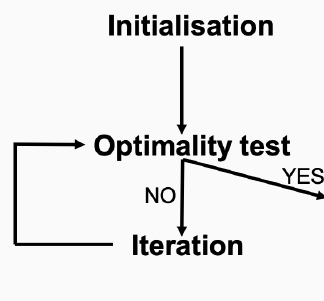
\includegraphics[width=0.6\columnwidth]{img/simplex_flow.png}
\end{center}
Quando l'esempio è stato risolto, questo diagramma di flusso è stato seguito attraverso due iterazioni fino a quando trovata la soluzione ottima.

\subsection{Concetto 3 - Come iniziare}
Quando possibile, l'inizializzazione del metodo del simplesso sceglie l'origine (variabili di decisione uguali a zero) per essere la soluzione CPF iniziale. Quando ci sono anche molte variabili decisionali per trovare graficamente una soluzione CPF iniziale, questa scelta elimina la necessità di utilizzare procedure algebriche per trovare e risolvere una soluzione CPF iniziale.\\
\\
Scegliere l'origine comunemente è possibile quando tutte le variabili decisionali hanno vincoli di non negatività, perché l'intersezione di questi limiti restituisce l'origine come soluzione del punto d'angolo. Questa soluzione è quindi una soluzione CPF a meno che è irrealizzabile perché viola uno o più vincoli. Se è irrealizzabile, sono necessarie procedure speciali per trovare la soluzione CPF iniziale.

\subsection{Concetto 4 - La scelta di una soluzione CPF migliore ad ogni iterazione}
Data una soluzione CPF, è molto più veloce dal punto di vista computazionale da raccogliere informazioni sulle soluzioni CPF adiacenti rispetto ad altre soluzioni CPF. Pertanto, ogni volta che il metodo del simplesso esegue un'iterazione per spostarsi dall'attuale soluzione CPF a una migliore, sceglie sempre una soluzione CPF adiacente a quella attuale. Nessun'altra soluzione CPF viene considerata. Di conseguenza, l'intero percorso che viene eseguito per raggiungere un'eventuale soluzione ottima è lungo i bordi della regione ammissibile.

\subsection{Concetto 5 - Quale soluzione CPF adiacente scegliere ad ogni iterazione}
Dopo aver identificato la soluzione CPF corrente, il metodo del simplesso esamina ciascuno dei bordi della regione ammissibile che si collegano a questa CPF e identifica il tasso di miglioramento in $Z$ che si otterrebbe spostandosi lungo il bordo. Tra i bordi con un tasso di miglioramento positivo in $Z$, sceglie quindi di spostarsi lungo quello con il tasso di miglioramento maggiore in $Z$. L'iterazione è completata risolvendo prima per la soluzione CPF adiacente all'altra estremità di questo bordo e quindi rietichettando questa soluzione CPF adiacente come l'attuale soluzione CPF per il test di ottimalità e (se necessario) l'iterazione successiva.\\
\\
Alla prima iterazione dell'esempio, lo spostamento da $(0, 0)$ lungo il bordo sull'asse $x_1$ darebbe un tasso di miglioramento in $Z$ di 3 ($Z$ aumenta di 3 per unità di aumento di $x_1$), mentre lo spostamento lungo il bordo sull'asse $x_2$ darebbe un tasso di miglioramento in $Z$ di 5 ($Z$ aumenta di 5 per unità di aumento di $x_2$), quindi si decide di spostarsi lungo quest'ultimo bordo. Alla seconda iterazione, l'unico arco proveniente da $(0, 6)$ che produrrebbe un tasso di miglioramento positivo in $Z$ è il bordo che porta a $(2, 6)$, quindi si decide di spostati poi lungo questo bordo.\\\\
In questo caso non è una buona idea spostarsi lungo il bordo con la maggiore velocità di miglioramento in $Z$. Infatti $Z = x_1 + 3x_2$. Se ci spostiamo lungo il bordo sull'asse $x_2$ abbiamo bisogno di due iterazioni ($A\rightarrow B \rightarrow C$), mentre se ci muoviamo lungo l'asse $x_1$ abbiamo solo bisogno di un'iterazione ($A \rightarrow C$).
\begin{center}
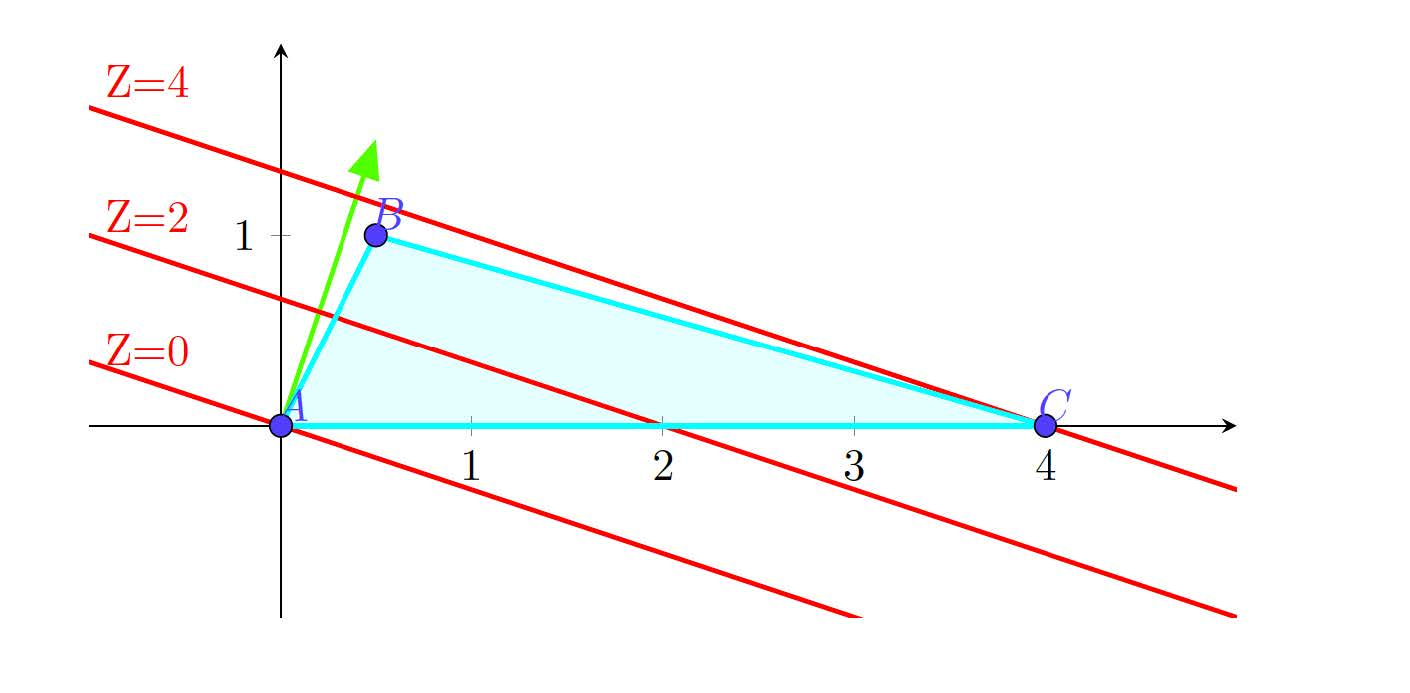
\includegraphics[width=0.5\columnwidth]{img/concept5.jpg}
\end{center}

\subsection{Concetto 6 - Come il test dell'ottimalità è svolto efficentemente}
Un tasso di miglioramento positivo in $Z$ implica che la soluzione CPF adiacente è migliore rispetto all'attuale soluzione CPF, mentre un tasso di miglioramento negativo in $Z$ implica che la soluzione CPF adiacente è peggiore. Pertanto, il test di ottimalità consiste semplicemente di verificare se uno qualsiasi degli spigoli fornisce un tasso di miglioramento positivo in $Z$. Se nessuno da una soluzione migliore, allora l'attuale soluzione CPF è ottima.\\\\
Nell'esempio, spostandosi lungo uno dei due lati da $(2, 6)$ diminuisce $Z$. Poiché vogliamo massimizza $Z$, questo fatto porta immediatamente alla conclusione che $(2, 6)$ è la soluzione ottima.\\

\subsection{Variazione di $Z$}
CPF $(2,6)$ è il punto di intersezione  tra $2x_2 = 12$ e $3x_1+2x_2 = 18$. Quest'ultimo limite può anche essere scritto come $x_1=6-{2\over3}x_2$. Quindi, quando $Z=3x_1+5x_2$ si muove lungo il vincolo abbiamo che $Z=3\cdot (6-{2\over3}x_2) + 5x_2$.\\
In $x_2=6, \ Z=36$. Quindi se $x_2 < 6, \ Z$ diminuisce e di conseguenza non è la via da prendere. Dal momento che anche in movimento lungo $x_2=6$ non permette di incrementare $Z$, ne consegue che $(2,6)$ è la soluzione ottima.\\
Analogamente, se andiamo a considerare $x_2=9-{3\over2}x_1$ otteniamo $Z=45-{9\over 2}x_1$. In $x_1=2, \ Z=36$ e questo valore decresce se $x_1$ aumenta.\\


%CAPITOLO
\clearpage
\section{04/10/2021- Soluzioni di base}
Un qualunque problema di programmazione lineare può essere formulato in forma standard  $max z = cz \ \ Ax=b \ \ (b \geq 0) \ \ x \geq 0$
Si supponga che $rank(A)=m$. Poiché $m<n$, eventualmente riordinando le colonne, si può porre $A=[B|N]$ dove 
\begin{itemize}
\item $B$ è una matrice non singolare $m\times n$ detta matrice delle colonne in base
\item $N$ è una matrice $m\times(n-m)$ detta matrice delle colonne fuori base
\end{itemize}
La matrice $B$ è composta da $m$ colonne di $A$ linearmente indipendenti che formano una base nello spazio vettoriale ad $m$ dimensioni delle colonne di $A$.\\
In corrispondenza di una scelta di $B$ ed $N$ si può partizionare anche il vettore delle $x$:
$$x=\left[\begin{array}{c}x_B\\x_N\end{array}\right] \begin{array}{l}m\ componenti\\n-m\ componenti\end{array}$$
\begin{itemize}
\item $x_B$ è detto vettore delle variabili in base (vettore di base)
\item $x_N$ è detto vettore delle variabili in fuori base
\end{itemize}
Il sistema di equazioni lineari $Ax=b$ si può riscrivere come: \\
$[B|N]\left[\begin{array}{c}x_B\\x_N\end{array}\right] = b \Rightarrow Bx_B+Nx_N = b \Rightarrow x_b = B^{-1}b-B^{-1}Nx_N$\\
Per ogni base $B$ ogni soluzione del sistema $Ax=b$ corrisponde a determinare il valore per m variabili $x_B$ avendo fissato arbitrariamente il valore per le restanti $n-m$ variabili.\\
Una scelta particolare importante è porre $x_V=0$, da cui si ottiene la corrispondente soluzione di base $x=\left[\begin{array}{c}x_B\\x_N\end{array}\right] = \left[\begin{array}{c}B^{-1}b\\0\end{array}\right]$\\
Se $B^{-1}b \geq 0$ si ottiene una soluzione di base ammissibile (BFS) per il sistema $Ax=B, \ x\geq 0$.\\

\subsection{Vertici e BFS}
\textbf{Teorema}: Dato un problema $Ax=b, \ x\geq 0$, una soluzione $x$ è un vertice del poliedro $P(A,b)$ se e solo se $x$ è una BFS\\
\textbf{Dim.} Un punto di un poliedro è un vertice (punto estremo) se e solo se soddisfa all’uguaglianza $n$ vincoli linearmente indipendenti, quindi basta dimostrare che ogni BFS soddisfa $n$ vincoli linearmente indipendenti tra $Ax = b,\ x \geq 0$.
Per definizione ogni BFS soddisfa all’uguaglianza $(n-m)$ vincoli $x \geq 0$ e gli $m$ vincoli di $Ax = b$. I vincoli stringenti sono linearmente indipendenti poiché la matrice dei loro coefficienti è certamente non singolare essendo nella forma $$\left(\begin{array}{cc}B&N\\0&I_{n-m}\end{array}\right)$$

\subsection{Problema}
Sia dato il problema:\\
$\begin{array}{rl}
max \ z = & 2x_1+x_2\\
 & x_1+x_2 \leq 5\\
 & -x_1 + x_2 \leq 0\\
 & 6x_1+2x_2 \leq 21\\
 & x_1,x_2 \geq 0
 \end{array}$\\
 Non è in forma standard, ma espresso solo in termini delle variabili strutturali (cioè quelle che hanno un immediata corrispondenza fisica col sistema reale che viene modellato).\\
 Lo si trasforma in forma standard introducendo le variabili di slack $x_3,x_4, x_5$\\
 $\begin{array}{rl}
max \ z =  & 2x_1+x_2\\
 & x_1+x_2 +x_3 = 5\\
 & -x_1 + x_2 + x_4 = 0\\
 & 6x_1+2x_2 + x_5 = 21\\
 & x_1,x_2, x_3, x_4, x_5 \geq 0
 \end{array}$\\
 $$A=\left[\begin{array}{ccccc}
 1&1&1&0&0\\
 -1&1&0&1&0\\
 6&2&0&0&1\\
 \end{array}\right] \ \ b=\left[\begin{array}{c}5\\0\\21\end{array}\right]$$
Limite superiore delle possibili basi ${5! \over 3!2!}=10$, ma non tutte le basi corrispondono ad una soluzione ammissibile BFS, nell'esempio solo 6 basi sono ammissibili.\\
Siccome i vertici sono 4, vi saranno BFS degeneri.\\
\paragraph{BFS}:
$$x_B^{(3)} = \left[\begin{array}{c}x_1\\x_2\\x_4\end{array}\right] \ \ \ \ \ B_3=\left[\begin{array}{ccc}1&1&0\\-1&1&1\\6&2&0\end{array}\right] \ \ \ \ \ B_3^{-1}={1\over4}\left[\begin{array}{ccc}-1&0&1\\6&0&-1\\-8&4&2\end{array}\right]$$
$$B_3^{-1}b=B_3^{-1}\left[\begin{array}{c}5\\0\\21\end{array}\right] = \left[\begin{array}{c}{11\over4}\\{9\over4}\\{1\over2}\end{array}\right] \Rightarrow p_3$$
$$x_B^{(2)}=\left[\begin{array}{c}x_1\\x_2\\x_5\end{array}\right] = \left[\begin{array}{c}{5\over2}\\{5\over2}\\1\end{array}\right] \Rightarrow p_2 \ \ \ \ \ x_B^{(4)}=\left[\begin{array}{c}x_1\\x_3\\x_4\end{array}\right] = \left[\begin{array}{c}{7\over2}\\{3\over2}\\{7\over2}\end{array}\right] \Rightarrow p_4$$
$$x_B^{(1)}=\left[\begin{array}{c}x_1\\x_3\\x_5\end{array}\right] = x_B^{(5)}=\left[\begin{array}{c}x_2\\x_3\\x_5\end{array}\right] = x_B^{(6)}=\left[\begin{array}{c}x_4\\x_3\\x_5\end{array}\right]  = \left[\begin{array}{c}0\\5\\21\end{array}\right] \Rightarrow p_1$$

\paragraph{Base non ammissibile}:
$$x_B^{(7)} = \left[\begin{array}{c}x_1\\x_2\\x_3\end{array}\right] \ \ \ \ \ B_7=\left[\begin{array}{ccc}1&1&1\\-1&1&0\\6&2&0\end{array}\right] \ \ \ \ \ B_3^{-1}={1\over8}\left[\begin{array}{ccc}0&-2&1\\0&6&1\\8&-4&-2\end{array}\right]$$
$$B_7^{-1}b=B_7^{-1}\left[\begin{array}{c}5\\0\\21\end{array}\right] = \left[\begin{array}{c}{21\over8}\\{21\over8}\\-{1\over4}\end{array}\right]$$
Analogamente sono basi non ammissibili 
$$\left[\begin{array}{c}x_2\\x_4\\x_5\end{array}\right] \ \ \ \ \left[\begin{array}{c}x_1\\x_4\\x_5\end{array}\right] \ \ \ \ \left[\begin{array}{c}x_2\\x_3\\x_4\end{array}\right]$$

\subsection{Variabili di surplus}
Se in un problema di PL ci sono dei vincoli di maggiore o uguale, per trasformare il problema in forma standard si introducono delle variabili di surplus con segno opposto, ad esempio, $$-3x_1+2x_2 \geq 5 \Longleftrightarrow -3x_1+2x_2 - x_6 = 5$$

\subsection{Soluzione PL}
Esplicitando la funzione obiettivo:
$$z=cx=[c_Bc_N]\left[\begin{array}{c}x_B\\x_N\end{array}\right] = c_Bx_B + c_Nx_N$$
e sostituendo l'espressione delle variabili di base $x_B=B^{-1}b-B^{-1}Nx_N$ si ottiene $z=c_BB^{-1}b-(c_BB^{-1}N-c_N)x_N$\\
Il valore dell'obiettivo corrispondente alla base $B$ è quindi $$z(B)=c_BB^{-1}b$$

%CAPITOLO 
\clearpage
\section{07/10/2021}
\subsection{Esercizio 1}
$$\begin{array}{cl}
max \ z = & 2x_1+x_2\\
 & x_2 \leq 10\\
 & 2x_1 + 5x_2 \leq 60\\
 & x_1+x_2 \leq 18\\
 & 3x_1+x_2 \leq 44\\
 & x_1,x_2 \geq 0
 \end{array}$$\\
 $A=(0,10) \rightarrow z_A = 10$\\
 $B=(5,10) \rightarrow z_B = 20$\\
 $C=(10,8) \rightarrow z_C = 28$\\
 $D=(13,5) \rightarrow z_D = 31$\\
 $E=({44\over 3}, 0) \rightarrow z_E = {88\over 3} \sim 29,\bar 3$\\

$\Longrightarrow D$ è la soluzione ottima

\subsection{Esercizio 2}
$$\begin{array}{cl}
max \ z = & 5x_1+7x_2\\
 & 2x_1-x_2 \leq -1\\
 & -x_1+2x_2 \leq -1\\
 & x_1,x_2 \geq 0
 \end{array}$$\\
 
 $\Longrightarrow$ La regione ammissibile è vuota
 
\subsection{Esercizio 3}
Dimostrare che la regione ammissibile è illimitata.
$$\begin{array}{c}
-x_1+3x_2 \leq 30\\
-3x_1+x_2 \leq 30\\
x_1,x_2 \geq 0
 \end{array}$$\\
 Se volessi massimizzare la funzione obiettivo $max\ z = 2x_1+x_2$ ci sono soluzioni ottime? NO\\
 Se invece volessi massimizzare $max \ z = x_1-x_2$? Non c'è
 Se faccio il $min\ z =  x_1-x_2$? Ho una soluzione ottima in $P=(0,10)$
 
\subsection{Esercizio 4}
$$\begin{array}{cl}
min \ z = & 40x_1+50x_2\\
 & 2x_1+3x_2 \geq 30\\
 & x_1+x_2 \geq 12\\
 & 2x_1+x_2 \geq 20\\
 & x_1,x_2 \geq 0
 \end{array}$$\\
 $A=(0,20) \rightarrow z_A = 1000$\\
 $B=({15 \over 2}, 5) \rightarrow z_B = 550$\\
 $C=(15,0) \rightarrow z_C = 600$\\
 
 $\Longrightarrow B$ è la soluzione ottima\\
 \\
 Come cambia la soluzione ottima se la funzione obiettivo diventa $min\ z_1=40x_1+70x_2$?\\
 $A=(0,20) \rightarrow z_A = 1400$\\
 $B=({15 \over 2}, 5) \rightarrow z_B = 650$\\
 $C=(15,0) \rightarrow z_C = 600$\\
 
$\Longrightarrow C$ diventa la soluzione ottima\\
\\
Come cambia la soluzione ottima se il terzo vincolo diventa $2x_1+x_2\geq 15$? La soluzione ottima diventa l'intersezione dei primi due vincoli.

\subsection{Esercizio 5}
$$\begin{array}{cl}
max \ z = & 8x_1+4x_2+6x_3+3x_4+9x_5\\
 & x_1+2x_2+3x_3+3x_4 \leq 180\\
 & 4x_1+3x_2+2x_3+x_4+x_5 \leq 270\\
 & x_1+3x_2+x_4+3x_5 \leq 180\\
 & x_1,x_2, x_3,x_4,x_5 \geq 0
 \end{array}$$\\
Mi diventa:
$$\begin{array}{cl}
max \ z = & 8x_1+4x_2+6x_3+3x_4+9x_5\\
 & x_1+2x_2+3x_3+3x_4 + s_1 = 180\\
 & 4x_1+3x_2+2x_3+x_4+x_5 + s_2 = 270\\
 & x_1+3x_2+x_4+3x_5 + s_3 =  180\\
 & x_1,x_2, x_3,x_4,x_5 \geq 0
 \end{array}$$\\
 La matrice A mi diventa:
 $$A=\left[\begin{array}{cccccccc}
 1&2&3&3&0&1&0&0\\
 4&3&2&1&1&0&1&0\\
 1&3&0&1&3&0&0&1\\
 \end{array}\right] \ \ b=\left[\begin{array}{c}180\\270\\180\end{array}\right]$$\\
 Nella soluzione ottima le variabili in base sono $x_3,x_1,x_5$
 $\Rightarrow B=\left[\begin{array}{ccc}
 3&1&0\\
 2&4&1\\
 0&1&3\\
 \end{array}\right]$\\
 $\Rightarrow B^{-1} = {1\over27}\left[\begin{array}{ccc}
 11&-3&1\\
 -6&9&-3\\
 2&-3&10\\
 \end{array}\right] \Rightarrow x_B = B^{-1}b = \left[\begin{array}{c}50\\ 30 \\50\end{array}\right]$
 
 \subsection{Esercizio 6}
$$\begin{array}{cl}
max \ z = & 4500x_1+4500x_2\\
 & x_1 \leq 1\\
 & x_2 \leq 1\\
 & 5000x_1+4000x_2 \leq 6000\\
 & 400x_1+500x_2 \leq 600\\
 & x_1,x_2 \geq 0
 \end{array}$$\\
 Mi diventa: $$\begin{array}{cl}
max \ z = & 4500x_1+4500x_2\\
 & x_1 + s_1= 1\\
 & x_2 + s_2 = 1\\
 & 5x_1+4x_2 + s_3 = 6\\
 & 4x_1+5x_2 + s_4 = 6\\
 & x_1,x_2 \geq 0
 \end{array}$$\\
 
 %CAPITOLO
 \clearpage
 \section{12/10/2021 - Il metodo del simplesso in forma matriciale}
 L'insieme dei vincoli e della funzione obiettivo possono essere scritti come un sistema lineare rispetto al quale si può supporre di aver individuato una base $B$ ammissibile
 $$\left[\begin{array}{cc}1 & -c^T\\0 & A\\\end{array}\right]\left[\begin{array}{c}z\\x\\\end{array}\right] = \left[\begin{array}{c}0\\b\end{array}\right] \Leftrightarrow \left[\begin{array}{ccc}1&-c_B^T & -c_N^T\\0&B&N\end{array}\right]\left[\begin{array}{c}z\\x_B\\x_N\end{array}\right]=\left[\begin{array}{c}0\\b\end{array}\right]$$
 La quasi (manca la prima colonna) matrice estesa di questo sistema composto dalle righe dei vincoli e dalla riga della funzione obiettivo è detta Tableau
 $$\left[\begin{array}{cc}-c^T&0\\A&b\end{array}\right]=\left[\begin{array}{ccc}-c_B^T & -c_N^T & 0\\B&N&b\end{array}\right]$$
 
 \subsection{Tableau}
\textbf{Tableau Iniziale}: prima della relativizzazione rispetto alla base $B$ scelta
\begin{center}
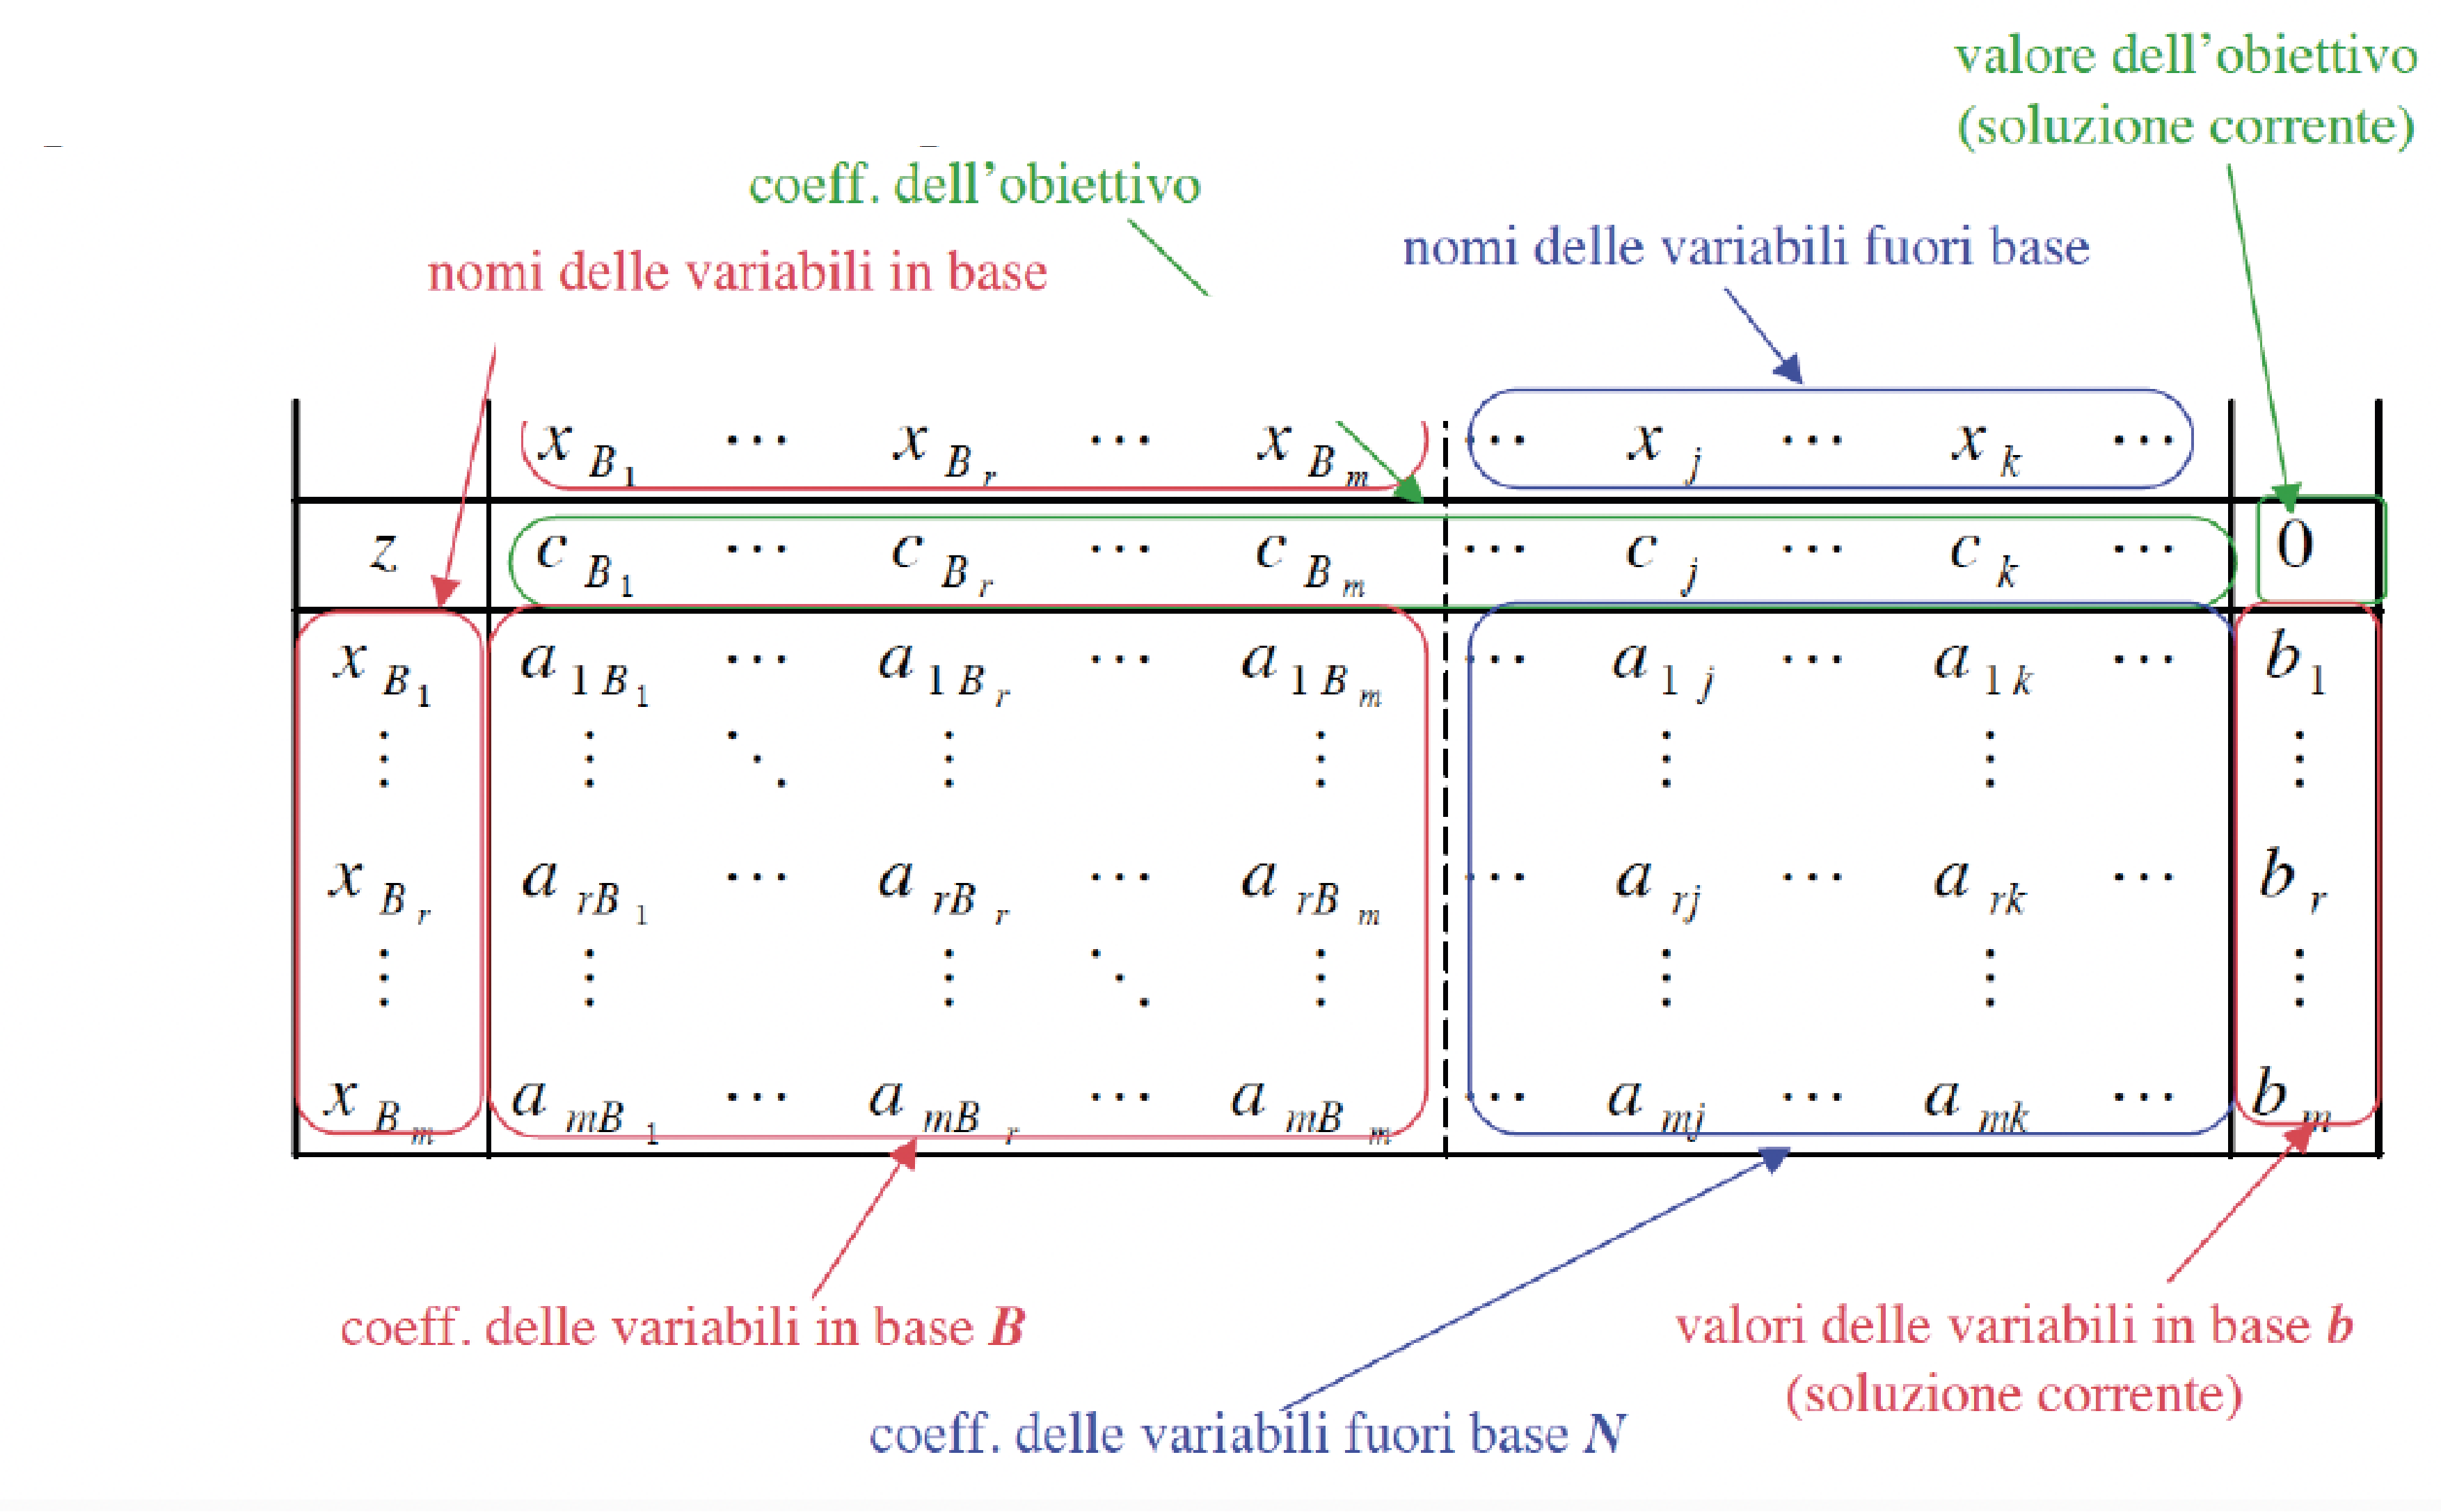
\includegraphics[width=0.6\columnwidth]{img/tableau_iniziale.png}
\end{center} 
\subsubsection{Tableau del problema $max \ z = 2x_1+x_2$}
 $\begin{array}{rl}
max \ z = & 2x_1+x_2\\
 & x_1+x_2 \leq 5\\
 & -x_1 + x_2 \leq 0\\
 & 6x_1+2x_2 \leq 21\\
 & x_1,x_2 \geq 0
 \end{array}$\\
Non è in forma standard, ma espresso solo in termini delle variabili strutturali (cioè quelle che hanno un immediata corrispondenza fisica col sistema reale che viene modellato).\\
 Lo si trasforma in forma standard introducendo le variabili di slack $x_3,x_4, x_5$\\
 $\begin{array}{rl}
max \ z =  & 2x_1+x_2\\
 & x_1+x_2 +x_3 = 5\\
 & -x_1 + x_2 + x_4 = 0\\
 & 6x_1+2x_2 + x_5 = 21\\
 & x_1,x_2, x_3, x_4, x_5 \geq 0
 \end{array}$\\
 Il tableau iniziale a colonne riordinate (sia noto che le colonne 3,4 e 1 formino una base iniziale ammissibile)
\begin{equation*}
\begin{array}{|c|ccccc|c|}
& x_1 & x_2 & x_3 & x_4 & x_5 & \\ \hline
z & -2 & -1 & 0 & 0 & 0 & 0\\ \hline
x_3 & 1 & 1 & 1 & 0 & 0 & 5\\
x_4 & -1 & 1 & 0 & 1 & 0 & 0\\
x_5 & 6 & 2 & 0 & 0 &1 & 21\\ \hline
\end{array} 
\Longrightarrow 
\begin{array}{|c|ccc:cc|c|}
& x_3 & x_4 & x_1 & x_5 & x_2 & \\ \hline
z & 0 & 0 & -2 & 0 & -1 & 0\\ \hline
x_3 & 1 & 0 & 1 & 0 & 1 & 5\\
x_4 & 0 & 1 & -1 & 0 & 1 & 0\\
x_1 & 0 & 0 & 6 & 1 & 2 & 21\\ \hline
& \multicolumn{3}{c}{B} & \multicolumn{2}{c}{N} & b
\end{array}
\end{equation*}
 
 \paragraph{Soluzione PL}: Esplicitando la funzione obiettivo:
 $$z=cx=[c_Bc_N]\left[\begin{array}{c}x_B\\x_N\\\end{array}\right]=c_Bx_B+c_Nx_N \ \ \ (1)$$
e sostituendo in (1) l'espressione delle variabili di base:
$$x_B=B^{-1}b-B^{-1}Nx_N \ \ \ (2)$$
si ottiene: $$z=c_BB^{-1}b - (c_BB^{-1}N-c_N)x_N \ \ \ \ (3)$$
il valore dell'obiettivo corrispondente alla base $B$ è quindi $z(B)=c_BB^{-1}b$\\
Le relazioni (2) e (3) esprimono rispettivamente i vincoli e la funzione obiettivo in funzione delle variabili fuori base.\\
Raccogliendo le $m+1$ equazioni di (2) e (3) in forma matriciale si ottiene
$$\left[\begin{array}{c}z\\x_B\end{array}\right]=\left[\begin{array}{c}c_BB^{-1}b\\B^{-1}b\end{array}\right] - \left[\begin{array}{c}c_BB^{-1}N-c_N\\B^{-1}N\end{array}\right]x_N$$
Il tableau corrispondente risulta essere
$$\left[\begin{array}{ccc}0 & c_BB^{-1}N-c_N &  c_BB^{-1}b \\ I & B^{-1}N & B^{-1}b\end{array}\right]$$
\begin{center}
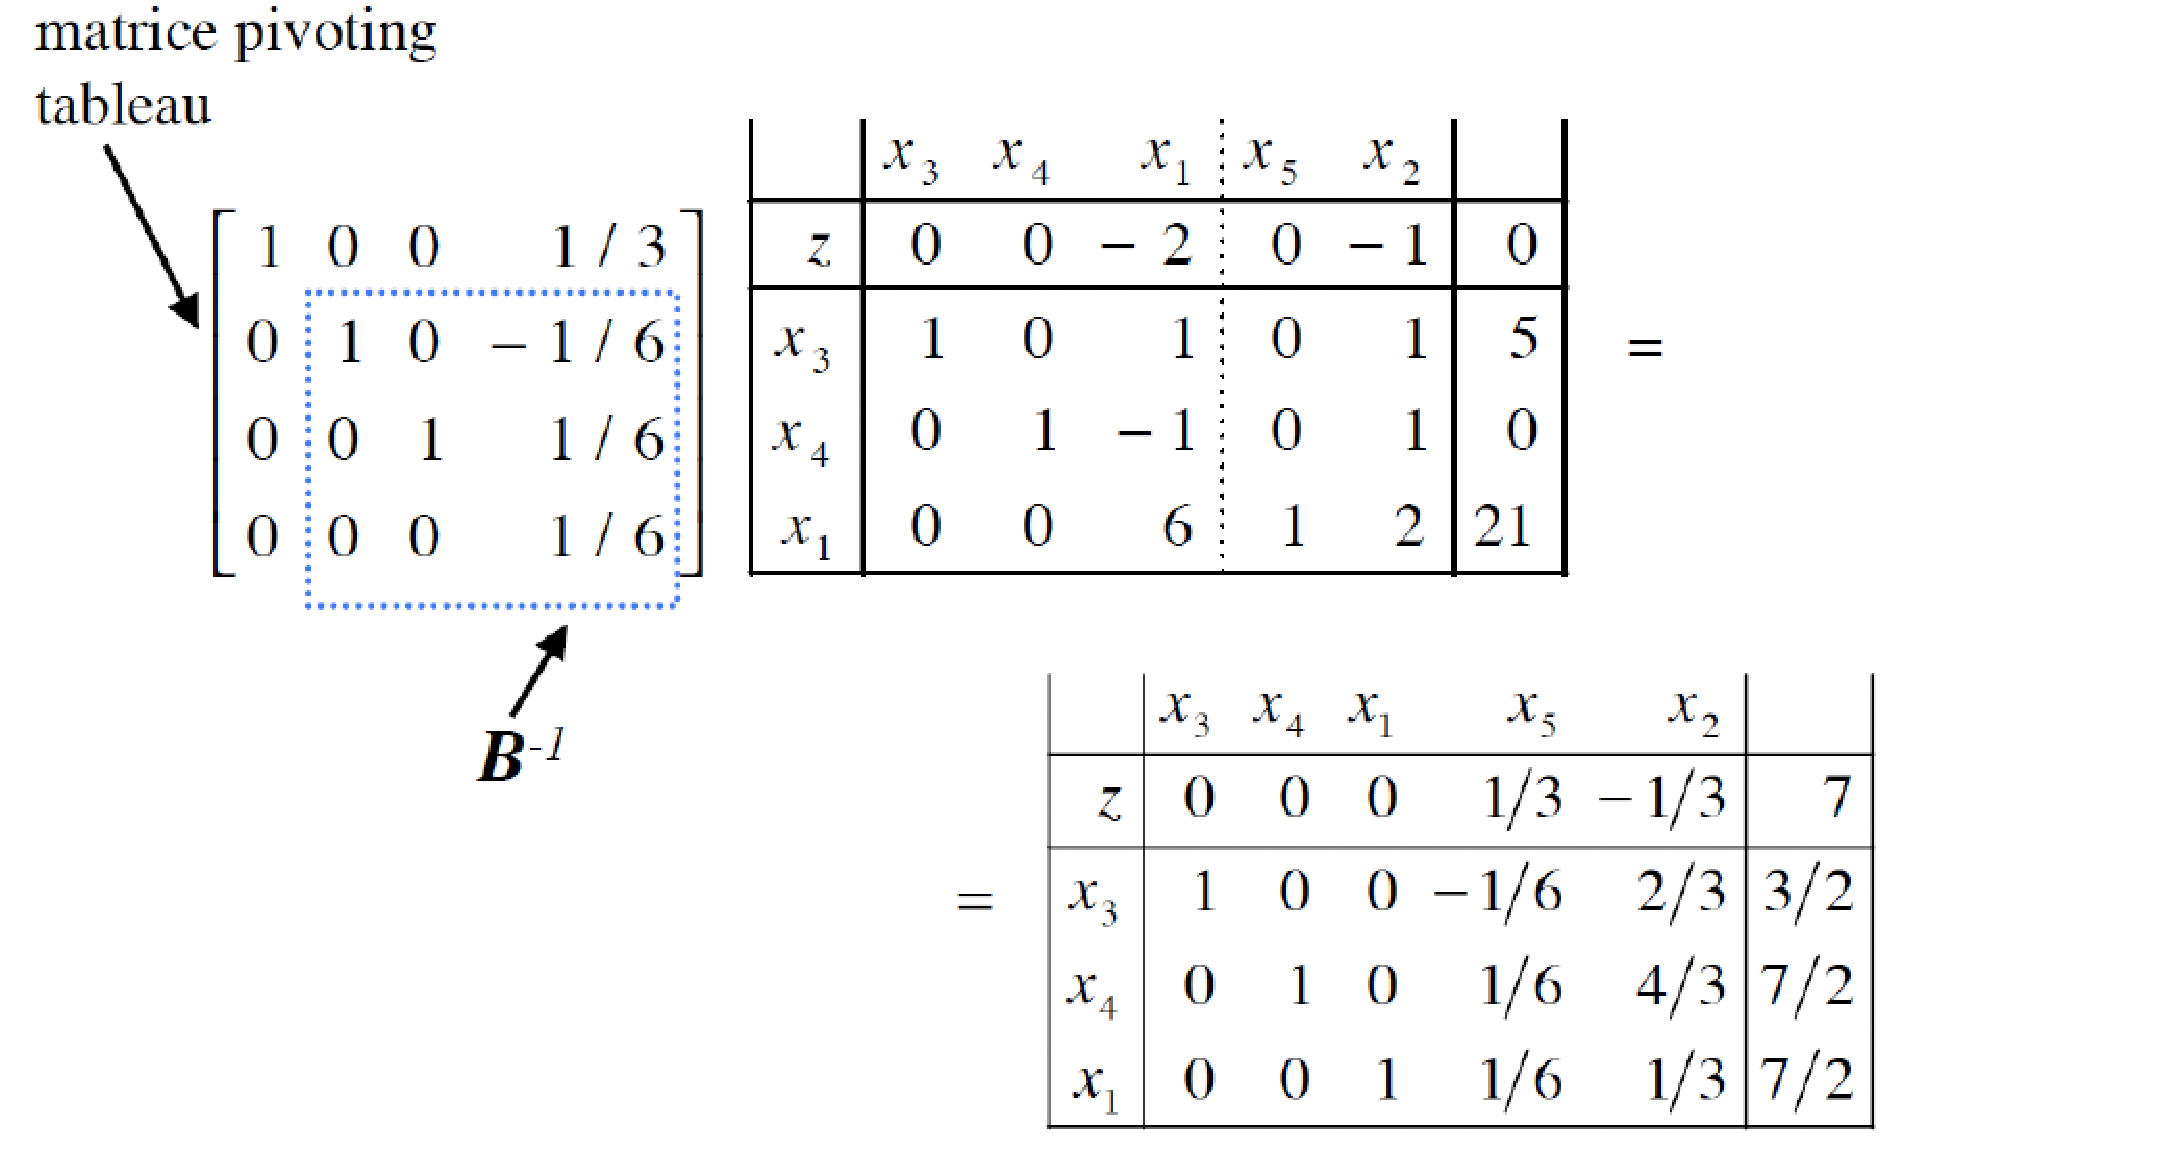
\includegraphics[width=0.5\columnwidth]{img/soles_tableau.png}
\end{center} 
Al fine di una scrittura più compatta sia $S$ l’insieme degli indici delle variabili in base, le colonne di $B$, e $R$ l’insieme degli indici delle variabili fuori base, le colonne di $N$, e si ponga
$$y_0=\left[\begin{array}{c}c_BB^{-1}b\\B^{-1}b\end{array}\right]=\left[\begin{array}{c}y_{00}\\y_{10}\\\vdots\\y_{m0}\end{array}\right] \ \ \ \ y_j = \left[\begin{array}{c}c_BB^{-1}A_j-c_j\\B^{-1}A_j\end{array}\right] = \left[\begin{array}{c}y_{0j}\\y_{1j}\\\vdots\\y_{mj}\end{array}\right] \ \forall j \in R$$
dove $A_j$ e $c_j$ sono rispettivamente la colonna $N$ ed il coefficiente di $c$ che moltiplicano la $j-ma$ variabili fuori base.\\
La componente $j-ma$ della BFS e l'obiettivo si possono quindi scrivere come
$$z=y_{00}-\sum_{j\in R}y_{0j}x_j$$
$$x_{Bi} = y_{i0} - \sum_{j\in R}y_{ij}x_j$$
\begin{center}
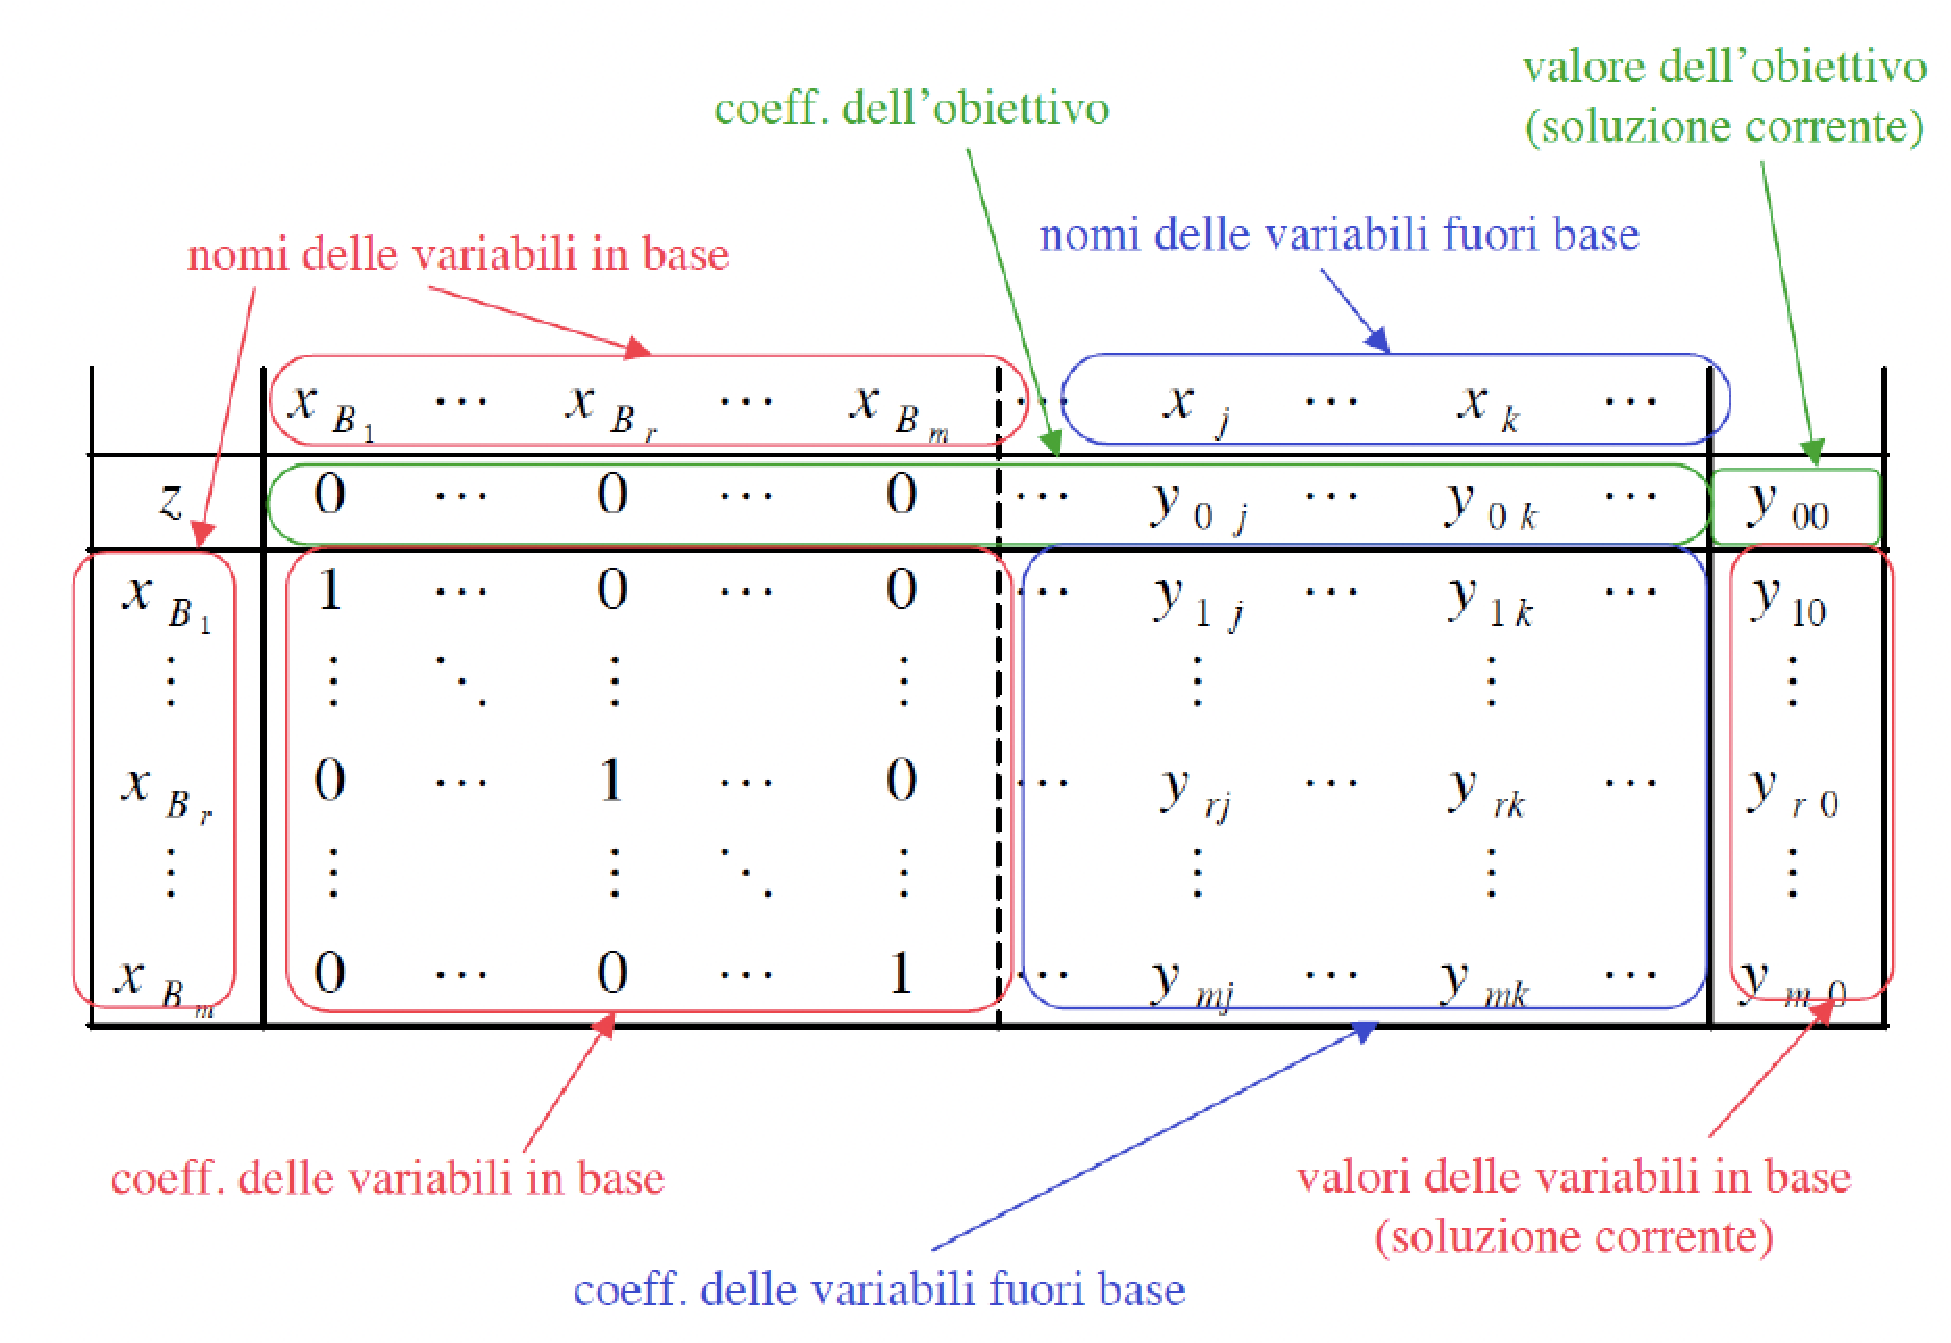
\includegraphics[width=0.5\columnwidth]{img/tableau.png}
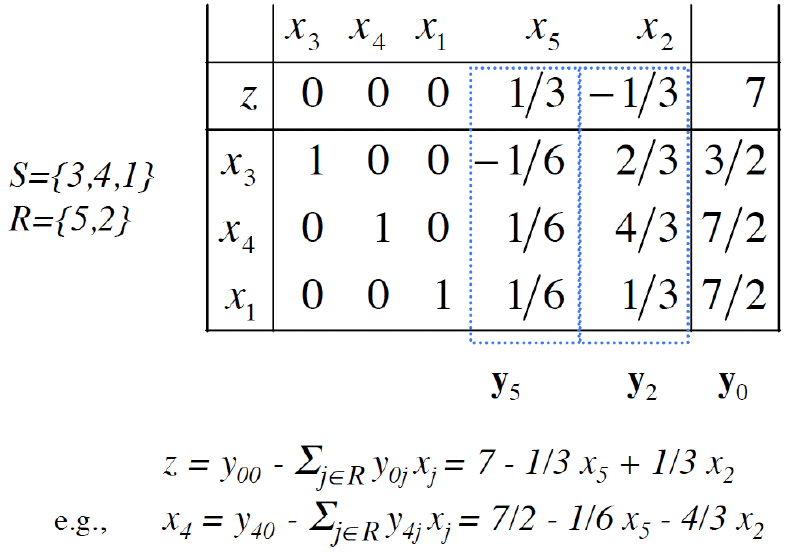
\includegraphics[width=0.5\columnwidth]{img/soles_tableau2.png}
\end{center} 
 
 \subsection{Verifica ottimalità soluzione corrente}
L'obiettivo $$z=y_{00}-\sum_{j\in R}y_{0j}x_j$$ data la corrente BFS vale $z(B)=y_{00}$.\\
Se esiste un coefficiente $y_{0k}<0\ (k\in R)$, facendo diventare positiva la variabile fuori base $x_k$ attualmente nulla, l'obiettivo aumenta di valore $$z=y_{00} - y_{0k}X_k > y_{00} = z(B)$$ allora, compatibilmente col rispetto dei vincoli, conviene aumentare il più possibile il valore della variabile $x_k$.
 
 \subsection{Rispetto ammissibilità}
Il vincolo generico associato all'elemento in base $i-esimo$
$$x_{Bi} = y_{i0} - \sum_{j\in R}y_{ij}x_j \geq 0$$
è rispettato dalla BFS corrente poiché $y_{i0}\geq 0$ e $x_j=0$ per $j\in R$.\\
Tale vincolo rispetto alla variabile fuori base che si vuole incrementare diventa
$$x_{Bi} = y_{i0} - y_{ik}x_k \geq 0$$
\begin{itemize}
\item Se il coefficiente $y_{ik}$ è non positivo, $x_k$ può incrementare a piacere senza violare la non negatività di $x_{Bi}$
\item Se il coefficiente $y_{ik}$ è positivo, $x_k$, per rispettare la non negatività può di $x_{Bi}$, può incrementare solo fino al valore $y_{i0} \over y_{ik}$
\end{itemize}
Il massimo valore che $x_k$ può assumere è quindi
$$x_k \leftarrow min\left\{{y_{i0} \over y_{ik}}:k\in R, y_{ik}>0\right\}$$

\subsubsection{Soluzione PL (esempio)}
Data la soluzione corrente $$z=7-{1\over3}x_5 +{1\over3}x_2$$
il coefficiente di $x_2$ è positivo, quindi conviene rendere il più positivo possible $x_2$, compatibilmente con i vincoli
$$x_3 = {3\over2}+{1\over6}x_5 - {2\over 3}x_2 \geq 0 \Rightarrow {3\over2}-{2\over3}x_2 \geq 0$$
$$x_4 = {7\over2}+{1\over6}x_5 - {4\over 3}x_2 \geq 0 \Rightarrow {7\over2}-{4\over3}x_2 \geq 0$$
$$x_1 = {7\over2}+{1\over6}x_5 - {1\over 3}x_2 \geq 0 \Rightarrow {7\over2}-{1\over3}x_2 \geq 0$$
Il valore massimo assumibile da $x_2$ è 
$$x_2 \leftarrow min\left\{{9\over4},{21\over8}, {21\over2}\right\} = {9\over 4}$$
\begin{center}
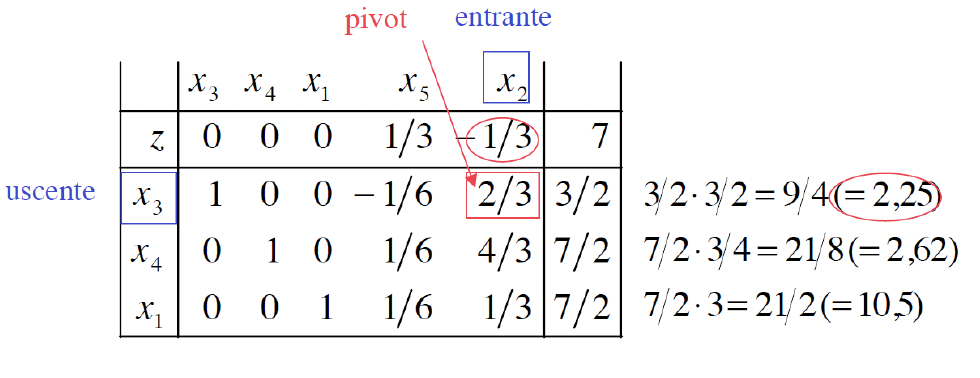
\includegraphics[width=0.5\columnwidth]{img/soles_amm.png}
\end{center} 
 
 \subsection{Cambio base}
 Sia $y_{rk}$ il valore per cui si ottiene il $min\left\{{y_{i0} \over y_{ik}}:k\in R, y_{ik}>0\right\}$.\\
 Tale valore è detto \textsl{pivot}.\\
 Se $x_k$ assume il massimo valore ammissibile allora i valori delle componenti di $x$, in particolare quelle in base che quindi dipendono da $x_k$, variano nel modo seguente
 $$\begin{array}{c}
 x_k \leftarrow {y_{r0}\over y_{rk}}\\
 x_j \leftarrow 0, \ \forall j \in R\setminus\{k\}\\
 x_{Bi} \leftarrow y_{i0}-y_{ik}\left({y_{r0}\over y_{rk}}\right), \ \forall i \in S
 \end{array}$$
 e quindi 
 $$x_{Br} \leftarrow 0$$
Per potere iterare il ragionamento conviene esprimere le soluzioni del sistema $Ax=b$, in funzione delle variabili che dopo l’aggiornamento hanno certamente valore nullo. Le equazioni associate alla componente $i-ma$ della BFS e l’obiettivo si dovranno quindi riscrivere come:
$$z=y_{00}-{y_{0k}y_{r0} \over y_{rk}} - \sum_{j\in R \setminus \{k\}}\left(y_{0j}-{y_{0k}y_{rj} \over y_{rk}}\right)x_j + {y_{0k}\over y_{rk}}x_{Br}$$
$$x_{Bi}=y_{i0}-{y_{ik}y_{r0} \over y_{rk}} - \sum_{j\in R \setminus \{k\}}\left(y_{ij}-{y_{ik}y_{rj} \over y_{rk}}\right)x_j + {y_{jk}\over y_{rk}}x_{Br}\ \ \forall i \in S \setminus \{r\}$$
$$x_k={y_{r0} \over y_{rk}} - \sum_{j\in R \setminus \{k\}}\left({y_{rj} \over y_{rk}}x_j + {1\over y_{rk}}x_{Br}\right)$$
ovvero si è cambiata la base
$$\begin{array}{c}
S \leftarrow S \cup\{k\}\setminus\{r\}\\
R \leftarrow R \cup\{r\}\setminus\{k\}\\
\end{array}$$

\subsubsection{Soluzione PL (esempio)}
\begin{center}
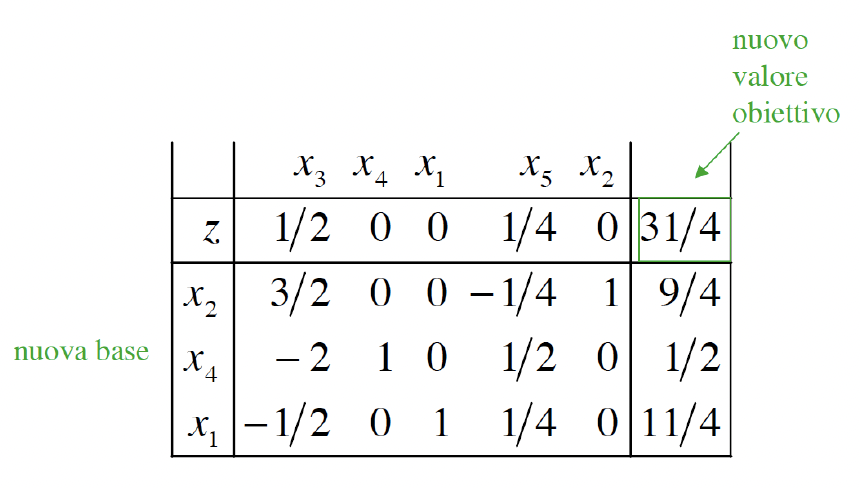
\includegraphics[width=0.5\columnwidth]{img/soles_cambiobase.png}
\end{center} 

\subsection{Iterazione}
Si ridefiniscono i vettori $y_j$ e $y_0$\\
Si verifica l'ottimalità o meno della base\begin{itemize}
\item Se esistono coefficienti $y_{0k}<0$ e $y_{rk} > 0$ si itera ponendo attenzione al cycling se $y_{rk}=0$
\item Se esistono dei coefficienti $y_{0k} < 0$, ma non esiste alcun $y_{rk}>0$, il problema è illimitato
\item Se non esiste alcun coefficiente $y_{0k}<0$ la soluzione corrente in base è ottima
\end{itemize}

\subsubsection{Soluzione PL (esempio)}
\begin{center}
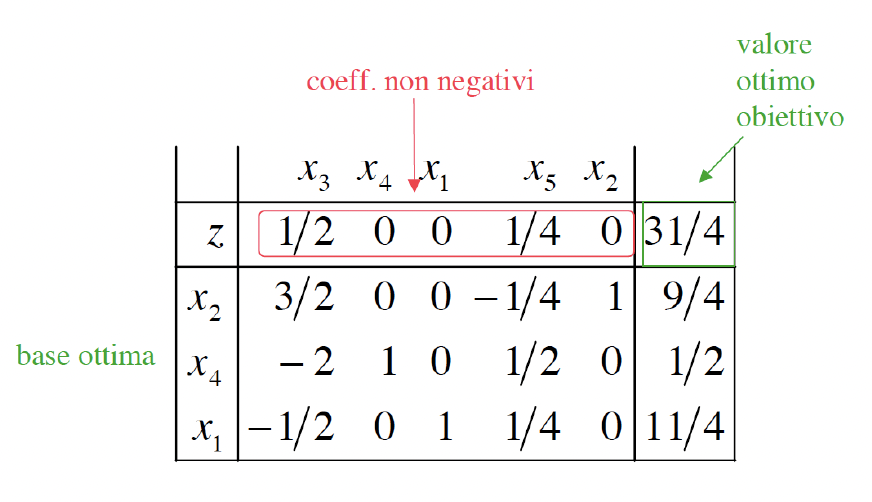
\includegraphics[width=0.5\columnwidth]{img/soles_iterazione.png}
\end{center} 

\subsection{Condizioni di ottimalità}
 Dato un problema di PL in forma standard una soluzione di base $x^*$ relativa alla base $B$, è ottima se si verificano le seguenti condizioni:
\begin{enumerate}
\item $B^{-1}b=y_0 \geq 0$ ammissibilità
\item $c_BB^{-1}A_j-c_j \leq 0 \Rightarrow y_{0j} \geq 0 \ \forall j$ non migliorabilità
\end{enumerate}
In realtà la condizione (2) può essere praticamente verificata per le sole variabili fuori base, infatti le variabili in base hanno per costruzione costi ridotti sempre nulli e quindi soddisfano
certamente la condizione data. La (2) quindi diventa $$c_BB^{-1}N_j-c_j \leq 0 \Rightarrow y_{0j} \geq 0\ \forall j \in R$$
 
 \clearpage
 \section{14/10/2021}
 \subsection{Problema}
  $$\begin{array}{cl}
max \ z = & 3x_1+5x_2\\
 & x_1\leq 4\\
 & 2x_2 \leq 12\\
 & 3x_1+2x_2 \leq 18\\
 & x_1,x_2 \geq 0\\
 \end{array}$$\\
 \'E equivalente  a: \\
$\begin{array}{cl}
max \ z = & 3x_1+5x_2\\
 & x_1+ x_3\leq 4\\
 & 2x_2 + x_4\leq 12\\
 & 3x_1+2x_2 + x_5 \leq 18\\
 & x_1,x_2,x_3,x_4,x_5 \geq 0\\
\end{array}$\\
\\
\textbf{Tableau Iniziale}\\
Scrivo $3x_1+5x_2$ in negativo perché considero $z-3x_1-5x_2=0$\\
\begin{center}
\begin{tabular}{c}
\\
$R_0$\\
$R_1$\\
$R_2$\\
$R_3$\\
\end{tabular}
\begin{tabular}{r|ccccc|c|}
& $x_1$ & $x_2$ & $x_3$ & $x_4$ & $x_5$\\
 \hline
 & -3 & -5 & 0 & 0 & 0 & 0\\
$x_3$ & 1 & 0 & 1 & 0 & 0 & 4\\
$x_4$ & 0 & 2 & 0 & 1 & 0 & 12\\
$x_5$ & 3 & 2 & 0 & 0 & 1 & 18\\
\end{tabular}\\
\end{center}
Se ponessi $x_1=x_2=0$ trovo che $x_3 =4, \ x_4=12, \ x_5 = 18$ ma \textsl{Non è la soluzione ottima perché ho due $x$ negative}\\
\begin{itemize}
\item $x_3=4-x_1$
\item $x_4 = 12 - 2x_2$
\item $x_5 = 18 - 3x_1-2x_2$
\end{itemize}
Faccio entrare in base $x_2$ ($x_1=0$):
\begin{itemize}
\item $x_3=4$
\item $x_4 = 12 - 2x_2$
\item $x_5 = 18 -2x_2$
\end{itemize}
in $x_2=6$ trovo che $x_4$ si annulla.\\
Dopo le operazioni \begin{itemize}
\item $R_2 = {1\over 2}R_2$
\item $R_0 = R_0 + 5R_2$
\item $R_3 = R_3 - 2R_2$
\end{itemize} il Tableau diventa:
\begin{center}
\begin{tabular}{c}
\\
$R_0$\\
$R_1$\\
$R_2$\\
$R_3$\\
\end{tabular}
\begin{tabular}{r|ccccc|c|}
& $x_1$ & $x_2$ & $x_3$ & $x_4$ & $x_5$\\
 \hline
& -3 & 0 & 0 & ${5\over2}$ & 0 & 30\\
$x_3$ & 1 & 0 & 1 & 0 & 0 & 4\\
$x_2$ & 0 & 1 & 0 & ${1\over2}$ & 0 & 6\\
$x_5$ & 3 & 0 & 0 & -1 & 1 & 6\\
\end{tabular}\\
\end{center}
\begin{itemize}
\item $x_1+x_3=4$
\item $x_2+{1\over2}x_4 = 6$
\item $3x_1-x_4+x_5=6$
\end{itemize}
Faccio entrare in base $x_1$ ($x_4=0$):
\begin{itemize}
\item $x_3= 4-x_1$
\item $x_2 = 6 - {1\over 2}x_4$
\item $x_5 = 6 -3x_1+x_4$
\end{itemize}
in $x_1=2$ trovo che $x_5$ si annulla.\\
Dopo le operazioni \begin{itemize}
\item $R_3 = {1\over 3}R_3$
\item $R_0 = R_0 + 3R_3$
\item $R_1 = R_1 - R_3$
\end{itemize} il Tableau diventa:
\begin{center}
\begin{tabular}{c}
\\
$R_0$\\
$R_1$\\
$R_2$\\
$R_3$\\
\end{tabular}
\begin{tabular}{r|ccccc|c|}
& $x_1$ & $x_2$ & $x_3$ & $x_4$ & $x_5$\\
 \hline
& 0 & 0 & 0 & ${3\over2}$ & 1 & 36\\
$x_3$ & 0 & 0 & 1 & ${1\over3}$ & $-{1\over3}$ & 2\\
$x_2$ & 0 & 1 & 0 & ${1\over2}$ & 0 & 6\\
$x_1$ & 1 & 0 & 0 & $-{1\over3}$ & ${1\over3}$ & 2\\
\end{tabular}\\
\end{center}
$\Longrightarrow$ Siamo alla soluzione ottima, perché tutte le variabili sono non negative e soprattutto non che qualora aumentassi una variabile la funzione obiettivo diminuisce.\\
\\
\\
\textbf{Soluzione del problema}: \href{https://units.enricolacchin.com/ricop21/problema_211014.xlsx}{EXCEL} - \href{https://units.enricolacchin.com/ricop21/problema_211014.pdf}{PDF}

%CAPITOLO
\clearpage
\section{18/10/2021 - Algoritmo del simplesso}
\begin{enumerate}
\item \textbf{Inizializzazione}: Determinare una soluzione di base ammissibile.
\item \textbf{Verifica dell'ottimalità}: Se $y_0\geq 0\  \forall j \in \R$, la soluzione corrente è ottima e l'algoritmo termina, altrimenti andare al passo 3.
\item \textbf{Scelta della variabile entrante in base}: Scegliere una variabile fuori base $x_k$ tale che $y_{0k} < 0$ ed andare al passo 4.
\item \textbf{Scelta della variabile uscente dalla base}: Scegliere una variabile $x_{Br}$ tale che ${y_{i0} \over y_{ir}} = min\left\{{y_{i0} \over y_{ik}} : j \in R, y_{ik} > 0\right\}$. Se $y_{ik} < 0 \ \forall i$, la soluzione del problema è illimitata, e l’algoritmo termina. Altrimenti si va al passo 5.
\item \textbf{Pivoting}: Risolvere i vincoli di uguaglianza esprimendo le nuove variabili in base $x_k$ e $x_{Bi} \ \forall i \not = k$, in funzione delle nuove variabili fuori base $x_{Bi}$ e $x_j\ \forall j \in R \setminus \{k\}$. La nuova BFS si ottiene ponendo le nuove variabili fuori base a zero. Andare al passo 2.
\end{enumerate}
Nell'algoritmo del simplesso si distingue una \textsl{fase I}, che consiste nel passo di inizializzazione in cui avviene individuata una prima BFS, e una \textsl{fase II}, che consiste nel determinare la BFS ottima e partire dalla prima BFS.\\
La fase II è stata già illustrata, la fase I viene illustrata in seguito.\\
La verifica se il problema è illimitato può anche venire fatta durante la fase II controllando tutte le colonne associate a costi ridotti positivi (e quindi coefficienti nel tableau negativi), se le colonne sono numerose questa verifica può essere onerosa.

\subsubsection{Fase I - Individuazione dell prima BFS}
In alcuni casi una prima base ammissibile è immediata. Si supponga infatti che il problema sia formulato come\\ $$\begin{array}{cl}max \ z = & cx\\
& Hx \leq b\\
& x \geq 0\\
\end{array}$$
con $b\geq 0$, allora la sua trasformazione in forma standard introduce delle variabili di slack $s$ le cui corrispondenti colonne formano la prima base ammissbile
$$\begin{array}{cl}max \ z = & cx\\
& Hx + Is = b\\
& x \geq 0, s\geq 0\\
\end{array}$$
Riordinando le colonne si ottiene $$A=[I|N] \ \ \ \ \ B=I \ \ \ \ \ N=H$$
dove chiaramente $$rank(A)=m \ \ \ \ B^{-1}b \geq 0$$


\subsection{Forma Canonica}
\textbf{Def}: Qualora un problema di PL in forma standard ha la matrice A che si può esprimere come $$A=[I|H], \ B=I \ e \ N=H$$ allora il problema è detto essere espresso in forma canonica.\\
\\
Non è immediato esprimere un problema di PL in forma canonica in presenza di disuguaglianze di verso opposto, infatti le variabili di surplus hanno coefficienti negativi, o in presenza di vincoli di uguaglianza.

\subsection{Esempio}
\begin{Parallel}{0.45 \textwidth}{0.45 \textwidth}
   \ParallelLText{Formulazione iniziale
$$\begin{array}{cl}max \ z = & 4x_1+x_2\\
& 3x_1+x_2=3\\
& 4x_1+3x_2 \geq 6\\
& x_1 + 2x_2 \leq 4\\
& x_1,x_2 \geq 0\\
\end{array}$$}
   \ParallelRText{Formulazione standard
$$\begin{array}{cl}max \ z = & 4x_1+x_2\\
& 3x_1+x_2=3\\
& 4x_1+3x_2 -x_3 = 6\\
& x_1 + 2x_2 +x_4 = 4\\
& x_1,x_2 \geq 0\\
\end{array}$$}
\end{Parallel}

\Sep \noindent
Questa formulazione standard non è UNA forma canonica
$$A=\left[\begin{array}{cccc}3&1&0&0\\4&3&-1&0\\1&2&0&1\end{array}\right]$$

\subsection{Fase I}
Se il problema è nella forma standard, ottenuto solo da vincoli di tipo $=$ e $\geq$, si introducono $m$ variabili artificiali $u$ e si formula il problema di fase I.
$$\begin{array}{rl}max \ z = & cx\\
& Hx \leq b\\
& x \geq 0\\
\end{array} \Rightarrow \ Fase\ I \ \ 
\begin{array}{rl}min \ w = & 1u\\
& Ax + Iu = b\\
& x \geq 0, u \geq 0\\
\end{array}$$
Per il problema di fase I è immediato determinare una base iniziale ammissibile.\\
Il problema di fase I ammette una soluzione ottima $w^*$ non negativa per costruzione
\begin{itemize}
\item Se $w^*>0$ allora il problema fase I non ha soluzioni ammissibili $x, u$ t.c. $u = 0$ e quindi non esiste $x$ t.c. $Ax + I0 = b \rightarrow Ax = b$, da cui il sistema $Ax = b$ non è compatibile e il problema di PL non ha soluzioni ammissibili
\item Se $w^*=0$ allora la componente della soluzione ottima $x^*, u^*$ è $u = 0$ e quindi $x^*$ è $Ax^*+I0 = b \rightarrow Ax^* =b$. Poiché $x^*$ ha al più m componenti non nulle essa può essere presa come prima BFS del problema originale.
\end{itemize}

\subsubsection{Esempio - Fase I}
$\begin{array}{cl}max \ z = & 4x_1+x_2\\
& 3x_1+x_2=3\\
& 4x_1+3x_2 -x_3 = 6\\
& x_1 + 2x_2 +x_4 = 4\\
& x_1,x_2 \geq 0\\
\end{array} \Rightarrow \begin{array}{cl}min \ w = & u_1+u_2 \Rightarrow max \ w = -u_1-u_2\\
& 3x_1+x_2 + u_1=3\\
& 4x_1+3x_2 +u_2 = 6\\
& x_1 + 2x_2 +x_4 = 4\\
& x_1,x_2 \geq 0\\
\end{array}$ \\
Data la presenza di una variabile di slack, bastano solo due variabili artificiali $(u_1,u_2)$.\\
$u_1,u_2,x_4$ è la base iniziale

\begin{center}
\begin{tabular}{c}
\\
$R_0$\\
$R_1$\\
$R_2$\\
$R_3$\\
\end{tabular}
\begin{tabular}{r|cccccc|c|}
& $x_1$ & $x_2$ & $x_3$ & $x_4$ & $u_1$ & $u_2$ \\
 \hline
& 0 & 0 & 0 & 0 & 1 & 1 & 0\\
$u_1$ & 3 & 1 & 0 & 0 & 1 & 0 & 3\\
$u_2$ & 4 & 3 & -1 & 0 & 0 & 1 & 6\\
$x_4$ & 1 & 2 & 0 & 1 & 0 & 0 & 4\\
\end{tabular}\\
\end{center}
Dopo le operazioni \begin{itemize}
\item $R_0 = R_0-R_1-R_2$
\end{itemize} il Tableau diventa:
\begin{center}
\begin{tabular}{c}
\\
$R_0$\\
$R_1$\\
$R_2$\\
$R_3$\\
\end{tabular}
\begin{tabular}{r|cccccc|c|}
& $x_1$ & $x_2$ & $x_3$ & $x_4$ & $u_1$ & $u_2$ \\
 \hline
& -7 & -4 & 0 & 0 & 0 & 0 & -9\\
$u_1$ & 3 & 1 & 0 & 0 & 1 & 0 & 3\\
$u_2$ & 4 & 3 & -1 & 0 & 0 & 1 & 6\\
$x_4$ & 1 & 2 & 0 & 1 & 0 & 0 & 4\\
\end{tabular}\\
\end{center}
Dopo un pò di passaggi il tableau finale sarà:
\begin{center}
\begin{tabular}{r|cccccc|c|}
& $x_1$ & $x_2$ & $x_3$ & $x_4$ & $u_1$ & $u_2$ \\
 \hline
& 0 & 0 & 0 & 0 & 1 & 1 & -9\\
$x_1$ & 1 & 0 & $1\over5$ & 0 & $3\over 5$ & $-{1\over5}$ & $3\over5$\\
$x_2$ & 0 & 1 & $-{3\over5}$ & 0 & $-{4\over5}$ & $3\over5$ & $6\over5$\\
$x_4$ & 0 & 0 & 1 & 1 & 0 & -1 & 1\\
\end{tabular}\\
\end{center}

%CAPITOLO
\clearpage
\section{19/10/2021 - Dualità}
\subsection{Un problema di produzione}
Un marchio produce $n$ differenti beni usando $m$ differenti materiali grezzi.\\
\begin{itemize}
\item Sia $b_i=1, \dots, m$ la quantità disponibile dell'$i-esimo$ materiale
\item Il $j-esimo$ bene, $j = 1 ,\dots , n$ richiede $a_{ij}$ unità del materiale $i-esimo$ e si traduce in un ricavo $c_j$ per unità prodotta.
\end{itemize}
L'impresa deve affrontare il problema di decidere quanto produrre di ciascun bene al fine di massimizzare i suoi ricavi totali.\\
La scelta della variabile di decisione è semplice. Sia $x_j,\ j = 1 ,\dots , n$ essere il quantità del $j-esimo$ bene da produrre.\\
\textbf{Formulazione primale}
$$\begin{array}{rl}max \ z = & c_1x_1+\dots+c_nx_n\\
& a_{i1}x_1+\dots +a_{in}x_n \leq b_i\\
& x_j \geq 0\\
\end{array}$$
\textbf{Variabili decisionali}: La quantità di beni prodotta $x_j \in \R$ per $1,\dots,n$. Assumiamo queste variabili continue.\\
\textbf{Funzione obiettivo}: Massimizzare il profitto di $$\sum_{j=1}^nc_jx_j$$
\textbf{Vincoli}: Per ogni materiale grezzo la somma del materiale usato per la produzione non deve superare il materiale disponibile
$$\sum_{j=1}^na_{ij}x_j\leq b_i \ \ for \ i=1,\dots,m$$
Per ogni bene, la quantità è sempre non negativa $$x_j\geq 0, \ j = 1, \dots, n$$

\subsubsection{Esempio}
$$\begin{array}{rl}max \ z = & 15x_1+10x_2\\
\textcolor{blue}{R_p} & x_1+x_2 \leq 2000\\
\textcolor{blue}{R_q} & x_1-0.5x_2 \leq 1000\\
\textcolor{blue}{R_r} & 2x_1+x_2 \leq 3000\\
& x_1, x_2 \geq 0\\
\end{array}$$
Notare che $R_q$ può essere anche ottenuto come sottoprodotto del secondo bene.

\subsubsection{Commenti sul problema primale}
Nell'affrontare un problema di produzione, prima ancora di decidere cosa produrre per ottenere il massimo profitto, ci si dovrebbe chiedere se è meglio produrre o se viceversa non conviene vendere (o utilizzare diversamente) le risorse disponibili.\\
La domanda da porsi è la seguente: \textsl{Qual è il prezzo minimo al quale tutte le risorse disponibili dovrebbe essere vendute piuttosto che prodotte?}\\
La risposta a questa domanda la troviamo nel problema duale

\subsection{Il duale di un problema di produzione}
Nell'ipotesi di linearità, il profitto complessivo che può essere ottenuto dalla vendita delle risorse è pari alla somma di i profitti che si ottengono vendendo le singole risorse, questi ultimi sono pari al prezzo unitario di vendita moltiplicato per quantità di risorse disponibili.\\
un prodotto $P_1$ dà un profitto di $15$ e consuma un'unità di $R_p$, un'unità di $R_q$ e $2$ unità di $R_r$. Pertanto, per rendere conveniente la vendita le risorse (o almeno rimanere alla pari) invece di produrre, la vendita complessiva di un'unità di $R_p$, una unità di $R_q$ e $2$ unità di $R_r$ deve fornire un guadagno non inferiore a $15$.\\
I prezzi di vendita delle risorse devono essere non negativi.

\subsection{Variabili duali e funzione obiettivo}
\begin{Parallel}{0.45 \textwidth}{0.45 \textwidth}
   \ParallelLText{\noindent
   \textcolor{red}{Variabili decisionali}\\
   Il prezzo unitario di ciascuna risorsa\\
   Queste sono variabili continue
   $$\pi_i \in \R,\ for\ i=p,q,r$$}
   \ParallelRText{\noindent
   \textcolor{red}{Funzione obiettivo}\\
   Il profitto ottenuto vendendo tutte le risorse disponibili
   $$2000\pi_p + 1000 \pi_q + 3000\pi_r$$}
\end{Parallel}

\subsection{Vincoli duali}
Per ogni bene il guadagno ottenuto dalla vendita delle risorse necessario per produrlo non deve essere inferiore al profitto ottenibile dalla vendita del bene stesso.
$$\sum_{i=1}^m a_{ij}\pi_j \geq c_j \ per \ j=1,2$$
Il prezzo di vendita delle risorse deve essere non negativo
$$\pi_i \geq 0, \ per\ i=p,q,r$$

\subsection{Formulazione del duale}
$$\begin{array}{rrl}\textcolor{blue}{Profitto} & min \ q = & 2000\pi_p + 1000 \pi_q + 3000\pi_r\\
\textcolor{blue}{Prodotto\ 1} & & \pi_p+\pi_q+2\pi_r \geq 15\\
\textcolor{blue}{Prodotto\ 2} & & \pi_p-0.5\pi_q+\pi_r \geq 10\\
& & \pi_p,\pi_q,\pi_r \geq 0\\
\end{array}$$
Quindi in termini generali 
$$\begin{array}{rl}min \ q = & \sum_{i=1}^m b_i\pi_i\\
 & \sum_{i=1}^ma_{ij}\pi_j \geq c_j \ per\ j=1,\dots,n\\
 & \pi_i \geq 0, \ per \ i=1,\dots, m\\
\end{array}$$
In forma matriciale
$$\begin{array}{rl}min \ q = & b^T\pi\\
 & A^T\pi \geq c\\
 & \pi \geq 0\\
\end{array}$$

\subsubsection{Commenti sul problema duale}
È intuitivamente evidente che
\begin{itemize}
\item Ogni soluzione praticabile per il duale permette di realizzare un profitto non inferiore al massimo profitto ottenuto risolvendo il problema primario (cioè, produrre). Quindi è conveniente vendere (o nel peggiore dei casi non perdi) se trovi qualcuno disposto a comprare tutto le risorse e pagarle insieme in modo da soddisfare i doppi vincoli;
\item La soluzione ottima del duale non può essere inferiore alla soluzione ottima del primale (altrimenti ci sarebbero i prezzi
che, pur soddisfacendo i vincoli, renderebbe la produzione ancora conveniente).
\end{itemize}

\subsection{Problema primale e problema duale}
Ad ogni problema LP (primale) è associato un problema duale
\SmallSep \noindent
\begin{Parallel}{0.45 \textwidth}{0.45 \textwidth}
   \ParallelLText{\noindent
   \textcolor{red}{Problema primale (P)}\\
   $$\begin{array}{rl}max \ z = & c_1x_1+\dots+c_nx_n\\
 & a_{11}x_1 + \dots + a_{1n}x_n \leq b_1\\
 & \vdots\\
 & a_{m1}x_1 + \dots + a_{mn}x_n \leq b_m\\
 & x_1,\dots,x_n \geq 0,\\
\end{array}$$
   $n$ variabili e $m$ vincoli}
   \ParallelRText{\noindent
   \textcolor{red}{Problema duale (D)}\\
   $$\begin{array}{rl}min \ w = & b_1\pi_1+\dots+b_m\pi_m\\
 & a_{11}\pi_1 + \dots + a_{m1}\pi_m \geq  c_1\\
 & \vdots\\
 & a_{1n}\pi_1 + \dots + a_{mn}\pi_m \geq c_n\\
 & \pi_1,\dots,\pi_m \geq 0,\\
\end{array}$$
   $m$ variabili e $n$ vincoli}
\end{Parallel}

\noindent
\textbf{Proprietà}: Il problema $D$ ha tante variabili quanti sono i vincoli in $P$ e tanti vincoli in quanto ci sono variabili in $P$.

\subsubsection{Forma matriciale}
In forma matriciale, vediamo che i vettori $b$ e $c$ scambiano le loro posizioni e il viene trasposta la matrice dei coefficienti $A$.

\SmallSep \noindent
\begin{Parallel}{0.45 \textwidth}{0.45 \textwidth}
   \ParallelLText{\noindent
   \textcolor{red}{Problema primale (P)}\\
   $$\begin{array}{rl}max \ z = & c^Tx\\
 & Ax \leq b\\
 & x \geq 0\\
 & x \in \R
\end{array}$$}
   \ParallelRText{\noindent
   \textcolor{red}{Problema duale (D)}\\
   $$\begin{array}{rl}min \ q = & b^T\pi\\
 & A^T\pi \geq c\\
 & \pi \geq 0\\
 & \pi \in \R
\end{array}$$}
\end{Parallel}

\subsubsection{Commenti}
La dualità nasce non solo da giustificazioni economiche, ma anche dall'applicazione di condizioni di Kuhn-Tucker a problemi di LP o da rilassamento Lagrangiano.11
La dualità è importante perché:
\begin{itemize}
\item Il problema duale corrisponde a una diversa visione dello stesso problema (per cui va sempre ricercata un'interpretazione economica della formulazione ottenuta);
\item Su di esso si basano algoritmi, come il Duale Simplesso e l'algoritmo Primale-Duale, alternativo al Simplesso (Primale), che sono utili per certi classi di problemi;
\item In alcuni casi può essere conveniente risolvere D invece di P (può essere meglio risolvere il problema con meno vincoli)
\end{itemize}

\subsubsection{Esempio}
\begin{Parallel}{0.45 \textwidth}{0.45 \textwidth}
   \ParallelLText{\noindent
   \textcolor{red}{Problema primale (P)}\\
   $$\begin{array}{rl}max \ z = & 2x_1+3x_2-x_3+7x_4\\
\textcolor{blue}{\pi_1} & 4x_1+3x_2-x_3+2x_4 \leq 35\\
\textcolor{blue}{\pi_2} & x_1+5x_2+6x_3+10x_4 = 28\\
\textcolor{blue}{\pi_3} & 2x_1+7x_2-2x_3+4x_4 \geq 15\\
& x_1 \geq 0,\ x_2 \ libera,\ x_3\leq 0, \ x_4 \geq 0\\
\end{array}$$} 
   \ParallelRText{\noindent
   \textcolor{red}{Problema duale (D)}\\
   $$\begin{array}{rl}min \ w = & 35 \pi_1+28 \pi_2 + 15\pi_3\\
\textcolor{blue}{x_1} & 4\pi_1+\pi_2 + 2\pi_3 \geq 2\\
\textcolor{blue}{x_2} & 3\pi_1+5\pi_2+7\pi_3 = 3\\
\textcolor{blue}{x_3} & -\pi_1+6\pi_2-2\pi_3 \leq -1\\
\textcolor{blue}{x_4} & 2\pi_1+10\pi_2 + 4\pi_3 \geq 7\\
& \pi_1 \geq 0,\ \pi_2 \ libera, \ \pi_3 \leq 0\\
\end{array}$$}
\end{Parallel}

\subsection{Teorema della dualità debole}
Se $x$ è una soluzione ammissibile del problema primale è anche una soluzione ammissibile del problema duale allora
$$c^Tx \leq b^t\pi$$
Prova infatti, $$c^Tx\leq(A^T\pi)^Tx = \pi^TAx \leq \pi^Tb=b^t\pi$$

\subsubsection{Corollario}
\begin{itemize}
\item[(a)] Se il valore ottimo nel primale è $+\infty$, allora il problema duale deve essere irrealizzabile
\item[(b)] Se il valore ottimo nel duale è $-\infty$, allora il problema primale deve essere irrealizzabile
\end{itemize}
\textbf{Dim.}: Supponiamo che il valore ottimo nel problema primale sia $+\infty$ e che il problema duale ha soluzione ammissibile . Per dualità debole, soddisfa $b^T\pi \geq c^Tx$ per ogni primale ammissibile $x$. Prendendo il massimo su tutto fattibile $x$, concludiamo $b^T\pi\geq +\infty$ . Questo è impossibile e mostra che il duale non può avere una soluzione praticabile, stabilendo così la parte (a). La parte (b) segue in maniera simmetrica.

\subsubsection{Corollario}
Siano $x$ e $\pi$ soluzioni ammissibili rispettivamente del primale e del duale, e supponiamo che $c^Tx = b^T$. Allora $x$ e $\pi$ sono soluzioni ottime di rispettivamente primale e duale.\\
\\
\textbf{Dim.}: Siano $x$ e come nell'enunciato del corollario. Per ogni soluzione ammissibile y del primale, il teorema della dualità debole dà $c^Tx=b^T\pi\geq c^Ty$, che dimostra che $x$ è ottimo. La dimostrazione dell'ottimalità di $\pi$ è simile.

\subsection{Teorema della dualità forte}
Se un problema di programmazione lineare ha una soluzione ottima, allora ce l'ha anche il duale, e i rispettivi valori ottimali sono uguali\\
\\
In altre parole, se $x^*$ è una soluzione ottima finita anche per il primale, il duale ha una soluzione ottima finita ed è sempre vero che $$c^Tx^* = b^T\pi^*$$

\subsection{Relazione tra Primale e Duale}
Ricordiamo che in un problema di programmazione lineare, esattamente uno dei seguenti tre le possibilità si verificheranno
\begin{itemize}
\item[(a)] C'è una soluzione ottima
\item[(b)] Il problema è “illimitato”, cioè il valore ottimo è $+\infty$ (per la massimizzazione problemi) o $-\infty$ (per problemi di minimizzazione)
\item[(c)] Il problema è irrealizzabile
\end{itemize}
Questo porta a nove possibili combinazioni per il primario e il duale:
\begin{center}
\begin{tabular}{|c||c|c|c|}
\hline
& Ottimo finito & Illimitato & Irrealizzabile\\ \hline
Ottimo finito & \textcolor{blue}{Possibile} & Impossibile & Impossibile\\
Illimitato & Impossibile & Impossibile & \textcolor{blue}{Possibile}\\
Irrealizzabile & Impossibile & \textcolor{blue}{Possibile} & \textcolor{blue}{Possibile}\\ \hline
\end{tabular}
\end{center}

\subsubsection{Complementary slackness}
Siano $x$ e $\pi$ soluzione ammissibile del problema primale e duale, rispettivamente. I vettori $x$ sono soluzioni ottime per i due rispettivi problemi se e solo se
$$\pi_i(b_i-a_i^Tx)=0\ \ \forall i$$
$$(\pi^TA_j -c_j)x_j = 0\ \ \forall j$$
dove $A_j$ è la $j-esima$ colonna e $a_i$ è l'$i-esima$ riga della matrice $A$.\\
\\
\textbf{Dim.}: se $(x, \pi)$ sono ottimi I vincoli dei problemi impongono che $\pi^Tb \geq \pi^TAx \geq c^Tx$. Poiché $x$ e $\pi$ sono ottimi $\pi^Tb = c^Tx$, quindi $\pi^Tx = \pi^TAx$ e quindi $\pi(b^T - Ax) = 0$. Analogamente, segue che $(\pi^TA -c^T )x = 0$. Infine, poiché $\pi \geq 0$, $b^T - Ax \geq 0,\ \pi^TA - c^T \geq 0, \ x \geq 0$, ne segue che ogni termine dello scalare i prodotti devono essere uguali a zero, cioè $\pi_i(a^T_ix - b_i) = 0 \ \ \forall i$ e $(c_j - \pi^TA_j )x_j = 0\ \ \forall j$.\\
Se le equazioni tengono, scrivendo le equazioni in forma compatta e per la coppia $(x, \pi)$ tale che $$\pi(b^T-Ax)= 0 \Rightarrow \pi b^T=\pi Ax$$
e $$(\pi^TA-c^T)x=0\Rightarrow \pi Ax=c^Tx$$
poiché $\pi^T b = \pi^T  Ax = c^T x$, allora $(x, \pi)$ è ottimo.

\subsubsection{Commenti}
Il teorema del gioco complementare può essere riformulato affermando che se un vincolo primario non è rigoroso (cioè è $<$) allora la variabile duale associata deve essere nulla, viceversa se la variabile duale non è nulla, il vincolo primario associato deve essere rigoroso (cioè, $=$).\\
Può succedere che il vincolo sia rigoroso e la variabile duale relativa sia nulla.

%CAPITOLO
\clearpage
\section{21/10/2021}
\subsection{Un problema rilassato}
Consideriamo la forma standard dei problemi
$$\begin{array}{rl}
min\ z & = c^Tx\\
& Ax = b\\
& x \geq 0
\end{array}$$
Che andremo a chiamare problema principale o primale, assumiamo che esista una $x*$ soluzione ottima. Andiamo a introdurre un problema rilassato nel quale il vincolo $Ax=b$ viene sostituito con $p^T(b-Ax)$, dove $p$ è un vettore con le stesse dimensioni di $b$. A questo punto affrontiamo il problema 
$$\begin{array}{rl}
min\ z & = c^Tx+p^T(b-Ax)\\
& x \geq 0
\end{array}$$
Sia $g(p)$ il valore ottimo per il problema rilassato, in funzione di vettore $p$. Il problema rilassato consente più opzioni di quelle presenti nel problema primale, e ci aspettiamo che $g(p)$ non sia maggiore rispetto al valore ottimo di $c^Tx*$. Infatti,
$$g(p)=min[c^Tx+p^T(b-Ax)] \leq c^Tx* + p^T(b-Ax*) = c^Tx*$$
Dove l'ultima equazione segue dal fatto che $x*$ è una soluzione ammissibile del problema primale e soddisfa $Ax*=b$.Quindi, ogni vettore $p$ porta a un limite inferiore $g(p)$ per il valore ottimo di $c^Tx*$.

\subsection{Un limite stretto}
Il problema $max \ g(p)$ (soggetto a nessun vincolo) può essere interpretato come una ricerca del limite inferiore più stretto possibile di questo tipo, ed è noto come problema duale.\\
Usando la definizione di $g(p)$, abbiamo
$$g(p)=min[c^Tx+p^T(b-Ax)] = p^Tb+ min(c^T-p^TA)x$$
Notiamo che $$min(c^T-p^TA)x=\begin{cases}
\begin{array}{ll}
0 & se\ c^T-p^TA \geq 0\\
-\infty & altrimenti\end{array}\end{cases}$$
Se massimizziamo $g(p)$ dobbiamo considerare solo quei valori di $p$ per cui $g(p)$ non è uguale a $-\infty$. Di conseguenza possiamo concludere che il problema duale è uguale a 
$$\begin{array}{rl}
max\ z & = p^Tb\\
& p^TA \leq c^T\\
\end{array}$$

\subsection{Il problema duale}
Nell'esempio, abbiamo iniziato con i vincoli di uguaglianza $Ax = b$ e abbiamo finito senza vincoli sul segno del vettore $p$. Se il problema principale avesse avuto invece vincoli di disuguaglianza della forma $Ax \geq b$, potrebbero essere sostituiti da, $Ax-s=s b,\ s \geq 0$. I vincoli di uguaglianza possono essere scritti nella forma
$$[A|-I]\left[\begin{array}{c}x\\s\end{array}\right]=b$$
Che porta i vincoli del duale
$$p^T[a|-I] \leq [c^T|0^T]$$
o equivalentemente
$$p^TA \leq c^T, \ p\geq 0$$
Se il vettore $x$ è libero piuttosto che vincolato dal segno, usiamo 
$$min(c^T-p^TA)x=\begin{cases}
\begin{array}{ll}
0 & se\ c^T-p^TA \geq 0\\
-\infty & altrimenti\end{array}\end{cases}$$
per finire con i vincoli $p^TA = c^T$ nel problema duale. Queste considerazioni motivano le relazioni tra primale-duale.

\begin{center}
\begin{tabular}{|c|c||c|c|}
\hline
Primale & massimizzo & minimizzo & Duale\\ \hline
Vincoli & $\begin{array}{c}\leq b_i\\\geq b_i\\=b_i\end{array}$ & $\begin{array}{c}\geq 0\\\leq 0\\libera \end{array}$ & Variabili\\ \hline
Variabili & $\begin{array}{c}\geq 0\\\leq 0\\libera \end{array}$ & $\begin{array}{c}\leq c_j\\\geq c_j\\=c_j\end{array}$ & Vincoli \\ \hline
\end{tabular}
\end{center}

\subsection{Analisi Sensitività}
Lo scopo principale dell'analisi di sensitività è identificare il parametri sensibili (cioè quelli che non possono essere modificati senza modificare il valore della soluzione ottimale). I parametri sensibili sono i parametri che devono essere valutati con particolare attenzione per ridurre al minimo il rischio di ottenere una soluzione ottimale errata. I parametri che vado a studiare sono $a_{ij}, b_i, c_j$ per $i=1,\dots, m$ e $j=1, \dots, n$

\subsection{Disponibilità delle risorse}
I problemi di programmazione lineare spesso possono essere interpretati come allocazione di risorse alle attività.\\
Quando i vincoli sono in forma $\geq$, abbiamo interpretato il $b_i$ (i membri di destra)
come i valori delle rispettive risorse messe a disposizione per il attività in esame.\\
n molti casi, i valori $b_i$ utilizzati nel modello iniziale possono effettivamente rappresentare
la decisione iniziale provvisoria della direzione su quante risorse saranno fornite dall'organizzazione alle attività prese in considerazione.\\
Da questa prospettiva più ampia, alcuni dei valori $b_i$ possono essere aumentati in
modello rivisitato, ma solo se si può presentare un caso estremamente vantaggioso per l'organizzazione.

\subsection{Prezzo ombra}
\textbf{Definizione}: Il prezzo ombra per la risorsa $i$ (indicato da $y_i^*$) misura il valore marginale di questa risorsa, cioè il tasso al quale la funzione obiettivo $z$ potrebbe essere aumentata (leggermente) aumentando la quantità di questa risorsa ($b_i$) messa a disposizione.\\\\
Nel caso di un vincolo funzionale in forma $=$ o $\geq$, il suo prezzo ombra è nuovamente definito come la velocità con cui $z$ potrebbe essere aumentato aumentando (leggermente) il valore di $b_i$, anche se l'interpretazione di $b_i$ ora sarebbe normalmente qualcosa di diverso dalla quantità di una risorsa messa a disposizione.\\

\subsubsection{Esempio}
\begin{center}
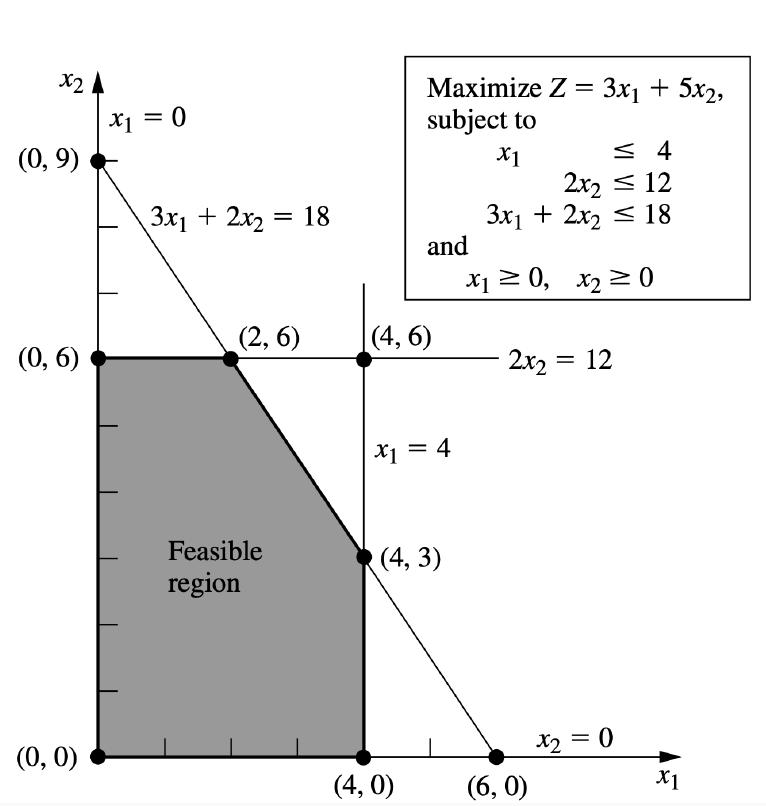
\includegraphics[width=0.5\columnwidth]{img/shadow_price_ex.png}
\end{center}
In questo esempio vediamo $\begin{array}{c}b_1=4\\b_2=12\\b_3=18\end{array}$\\
Cosa succederebbe se incrementassimo di 1 $b_2$ e la portassimo quindi a un valore $b_2=13$?
\begin{center}
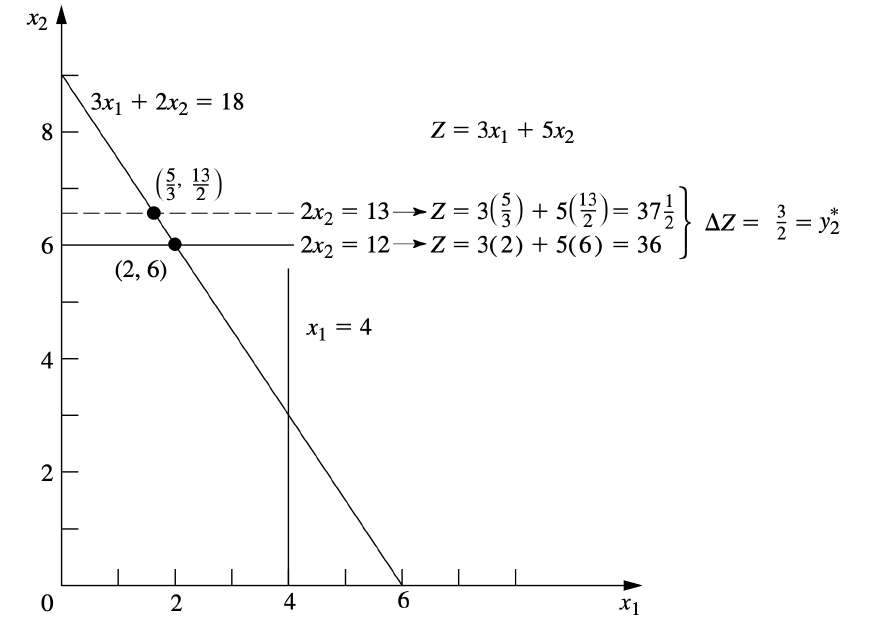
\includegraphics[width=0.5\columnwidth]{img/shadow_price_exbis.png}
\end{center}
Il grafico ci mostra che il prezzo ombra è $y_2^* = {3\over2}$ per la seconda risorsa. I due pallini neri sono le due soluzioni ottimali al variare del vincolo. Mettendo queste due soluzioni nella funzione obiettivo si nota che esse varia, per l'appunto di $y_2^* = {3\over2}$.
Abbiamo dimostrato che $y_2^* = {3\over2}$ è il valore secondo il quale la funzione obiettivo $z$ incrementa se vado a incrementare il valore di $b_2$. Tuttavia, dimostra anche il comune
fenomeno che questa interpretazione vale solo per un piccolo aumento di $b_2$. Una volta che $b_2$ è aumentato oltre 18, la soluzione ottima rimane a $(0, 9)$ con nessun ulteriore aumento della funzione obiettivo $z$.\\
In altre parole, $z=45$ per ogni $b_2$ tale che $b_2 \geq 18$ perché il vincolo $2x_2=b_2$ diventa ridondante.\\
\\
Notiamo che $y_1^*=0$ perché il vincolo sulla risorsa 1, $x_1 \leq 4$, non è vincolante per la soluzione ottima $(2,6)$, c'è un surplus di questa risorsa. Di conseguenza, aumentando $b_1$ oltre a $4$ non si può ottenere una nuova soluzione ottima con valore maggiore della funzione obiettivo.\\
Al contrario, i vincoli sulle risorse 2 e 3, $2x_2 \leq 12$ e $3x_1 + 2x_2 \leq 18$, sono vincoli vincolanti (vincoli che valgono con uguaglianza alla soluzione ottimale). Perché l'offerta limitata di queste risorse ($b_2 = 12$, $b_3 = 18$) vincola $z$ dall'essere ulteriormente aumentata, hanno prezzi ombra positivi. Possiamo facilmente dimostrare che $y_3^*=1$.\\
Gli economisti si riferiscono a tali risorse come beni scarsi, mentre le risorse disponibili in eccedenza (come la risorsa 1) sono beni gratuiti (risorse con a prezzo ombra zero).

\subsection{Problema primale e duale}

\begin{Parallel}{0.45 \textwidth}{0.45 \textwidth}
   \ParallelLText{Problema primale
$$\begin{array}{rl}
max \ z & = 3x_1 + 5x_2\\
&x_1 \leq 4\\
&2x_2 \leq 12\\
&3x_1 + 2x_2 \leq 18\\
&x_1,x_2 \geq 0
\end{array}$$
La soluzione ottima è $$x_1^*=2, \ x_2^*=6, \ z^* = 36$$}
   \ParallelRText{Problema duale
$$\begin{array}{rl}
min \ w & = 4\pi_1 + 12\pi_2 + 18\pi_3\\
&\pi_1+3\pi_3 \geq 3\\
&2\pi_2 +2\pi_3 \geq 5\\
&\pi_1,\pi_2, \pi_3 \geq 0
\end{array}$$
Dalla dualità forte sappiamo che $w^*=36$. Come possiamo trovare le variabili ottimali?}
\end{Parallel}

\Sep \noindent
Le variabili di slack complementari sono:
$$\begin{array}{cl}
\pi_i^*(b_i-a_i^Tx^*)=0  & \forall i\\
(\pi^{T*}A_j-c_j)x_j^* = 0 & \forall j
\end{array}$$

\begin{Parallel}{0.45 \textwidth}{0.45 \textwidth}
   \ParallelLText{Che nel nostro caso diventa
   $$\begin{array}{r} 
   \pi_1^*(4-x_1*)=0\\
   \pi_2^*(12-2x_2^*)=0\\
   \pi_3^*(18-3x_1^*-2x_2^*)=0\\
   (\pi_1^* + 3\pi_3^* - 3)x_1^*=0\\
   (2\pi_2^*+2\pi_3^*-5)x_2^* = 0
   \end{array}$$
   Ne consegue che
   $$\begin{array}{r} 
   \pi_1^*=0\\
   (\pi_1^* + 3\pi_3^* - 3)=0\\
   (2\pi_2^*+2\pi_3^*-5) = 0
   \end{array}$$}
   \ParallelRText{Se $x_1^*=2,\ x_2^*=6$ allora
   $$\begin{array}{r}
   2\times \pi_1^* = 0\\
   0 \times \pi_2^*=0\\
   0 \times \pi_3^* = 0\\
   2 \times (\pi_1^*+3\pi_3^* -3)=0\\
   6 \times (2\pi_2^* + 2\pi_3^* - 5)=0
   \end{array}$$
   che è
   $$\begin{array}{r}
   \pi_1^* = 0\\
   \pi_3^* = 1\\
   \pi_2^*={3\over2}\\
   \end{array}$$}
\end{Parallel}

\MidSep \noindent
In fatti, $w^*=4\times 0 + 12 \times {3\over 2} + 18 \times 1 = 36$. In aggiunta notiamo che $y_1^*=\pi_i^*$ per $i=1,2,3$.\\
Le variabili ottimali del duale sono uguali al prezzo ombra.

\subsection{Variabili duale e Prezzo ombra}
Abbiamo mostrato che ogni variabile duale ottima rappresenta la "velocità" con cui la funzione obiettivo $z$ varia al variare del corrispondente valore di destra.\\
Se si varia un membro destro, il valore delle variabili duali ottimali rimane costante fintanto che la soluzione ottima giace sull'intersezione della stessa limiti di vincolo.\\
Nel nostro esempio
\begin{itemize}
\item Se $b_2 > 18$ la soluzione ottima è sempre $(0,9)$. La variabile duale ottimale è $(0,0,{5\over2})$
\item Se $b_2$ varia nell'intervallo $6<b_2<18$ la soluzione ottima giace sull'intersezione tra $2x_2 = b_2$ e $3x_1+2x_2=18$ e le variabili della soluzione ottima duale sono $(0,{3\over2},1)$
\item Se $0<b_2<6$ la soluzione ottima giace sui vincoli $2x_2=b_2$ e $x_1=4$. Le soluzioni delle variabili duali sono $(3,{5\over2},0)$
\item Se, invece, $b_2=6$ o $b_2=18$ la soluzione si dice degenere. 
\end{itemize}
\begin{center}
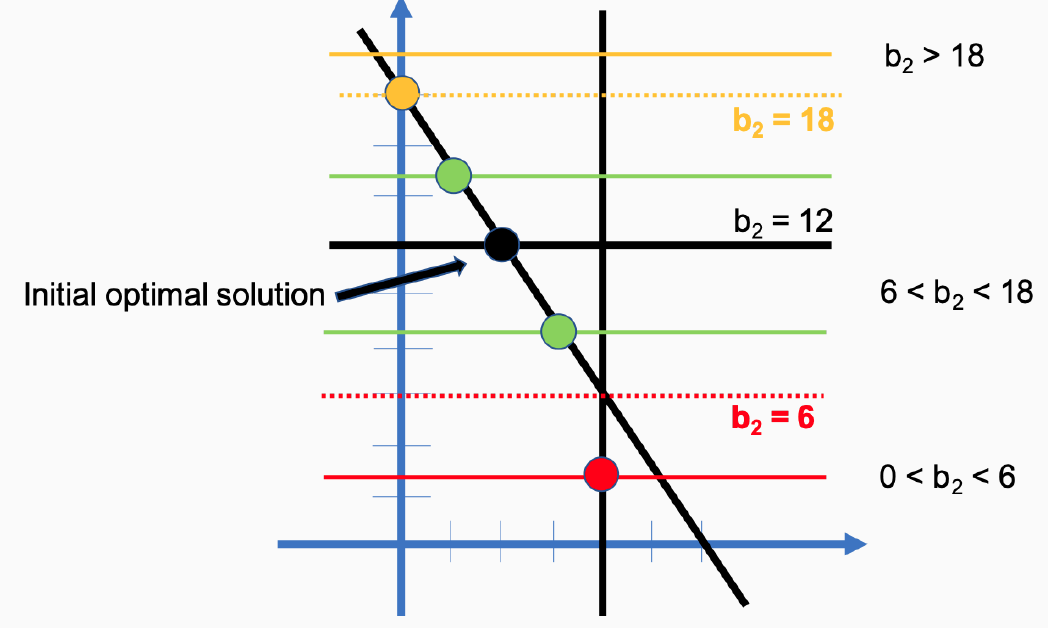
\includegraphics[width=0.5\columnwidth]{img/shadow_price_extris.png}
\end{center}

\subsection{Variazione dei coefficienti della funzione obiettivo}
\begin{center}
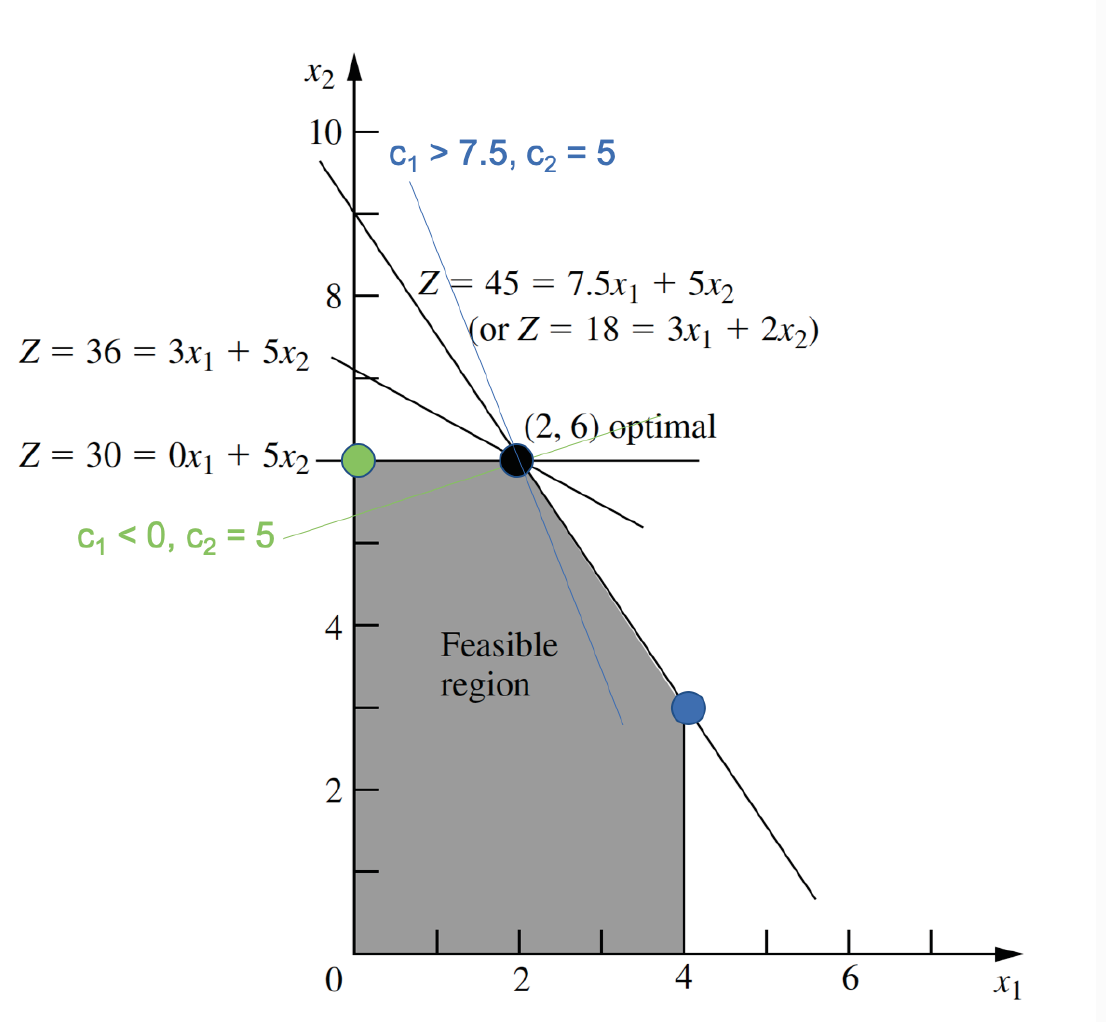
\includegraphics[width=0.5\columnwidth]{img/z_variation.png}
\end{center}
Il grafico dimostra l'analisi della sensibilità di $c_1$ e $c_2$ per il nostro problema. Partendo dalla linea della funzione obiettivo (dove $c_1=3, \ c_2=5$, e la soluzione ottima è $(2,6)$). Le altre due linee nere mostrano gli estremi nei quali la funzione può variare e far si che la soluzione ottima rimanga $(2,6)$. Quindi \begin{itemize}
\item Con $c_2=5$ il range di estensione per $c_1$ è $0 \leq c_1\leq 7,5$
\item Con $c_1=3$ il range di estensione per $c_2$ è $c_2 \leq 2$
\end{itemize}

%CAPITOLO
\clearpage
\section{26/10/2021 - Teoria dei giochi (strategie pure)}
\subsection{Teoria dei giochi}
Fino a questo momento abbiamo analizzato prevalentemente problemi in cui il decisore era unico. Mostriamo ora casi in cui si abbiano più decisori che agiscono sullo stesso sistema ma con interesse fra loro non coincidenti, cioè in situazioni di conflitto. Il risultato di ogni decisore viene a dipendere dalle sue scelte ma anche da quelli degli altri decisori, il che è appunto ciò che accade in situazioni di conflitto.\\
Il primo tentativo sistematico di studiare questi problemi è stato condotto dal matematico Von Neumann negli anni che precedettero la seconda guerra mondiale e ha dato vita ad una fortunata branca della matematica applicata nota con il nome di \textcolor{red}{teoria dei giochi}.
\subsubsection{Terminologia}
In un gioco ciascuno dei decisori che vengono normalmente chiamati \textsl{giocatori} ha una funzione obiettivo (che può essere un costo o un beneficio) detta spesso \textcolor{red}{funzione di payoff}.\\
Esistono giochi anche con $n$ giocatori ognuno dei quali fa le sue scelte conoscendo completamente o solo in parte (informazione incompleta) le caratteristiche del problema.\\
Un gioco è detto \textcolor{red}{deterministico} se in esso non interviene il caso.\\
Il risultato del gioco deterministico, cioè il valore delle varie funzioni di payoff $f_i(x_1,x_2,\dots,x_n)$ per tutti gli $n$ giocatori, è perfettamente noto una volta che siano note le scelte dei vari giocatori.\\
Se ogni giocatore ha a disposizione un numero infinito di scelte il gioco si dice \textcolor{red}{continuo} per distinguerlo dal caso, detto \textcolor{red}{discreto}, in cui le variabili hanno numero finito di possibili conclusioni.\\
A seconda del tipo di saturazione si possono avere \begin{itemize}
\item Casi di conflitto puro
\item Casi in cui è possibile la cooperazione tra i giocatori
\item Casi in cui alcuni giocatori possono coalizzarsi con altri
\end{itemize}

\subsection{Giochi a somma nulla}
\textcolor{blue}{\textbf{Definizione}:} Se la somma delle funzioni di payoff è uguale a 0 diremo che si tratta di un gioco a \textcolor{red}{somma nulla}.\\
Se invece è diversa da 0 diremo che il gioco è a \textcolor{red}{somma non nulla}.\\
\\
Esiste una sostanziale differenza tra questi due casi: nel secondo infatti accade che si abbiamo soluzioni vantaggiose per tutti gli $n$ giocatori, purché questi cooperino, mentre nel primo caso ciò è escluso: qualcuno vince qualcuno perde.

\subsubsection{Due giocatori}
Nel caso particolare di due giocatori se risulta $$f_1+f_2=0$$ e quindi $f_1=-f_2$ si dice che il gioco è a due persone a somma nulla. In questo caso non è possibile né la cooperazione né la 
coalizione fra i due giocatori perché ciò che un giocatore vince viene perso dall'altro.

\subsubsection{Un gioco stupido} 
Lucy e Linus giocano. Ciascuno di loro compie l'azione di mostrare contemporaneamente all'altro uno o due dita: Linus paga a Lucy tanti centesimi quant'è la somma delle dita.\\
Si tratta di un gioco con scarse probabilità di successo poiché nessuna persona sana di mente accetterebbe il ruolo di Linus.\\
Le coppe di strategie possibili sono quattro e precisamente, indicando la prima scelta di Lucy e poi quella di Linus:
\begin{itemize}
\item 1 dito - 1 dito
\item 1 dito - 2 dita
\item 2 dita - 1 dito
\item 2 dita - 2 dita
\end{itemize}
Il gioco si esaurisce con una coppia di mosse dei due giocatori dopodiché si può stabilire il risultato.\\
Le vincite di Lucy (che poi sono le perdite di Linus) si possono esprimere mediante una matrice $2\times2$ molto semplice
\begin{center}
\begin{tabular}{|cc|cc|} 
\cline{3-4}
\multicolumn{1}{c}{}                                             &    & \multicolumn{2}{c|}{Linus}  \\
\multicolumn{1}{c}{}                                             &    & $1d$ & $2d$                     \\ 
\hline
\multirow{2}{*}{\begin{tabular}[c]{@{}c@{}}Lucy \\\end{tabular}} & $1d$ & 2  & 3                      \\
                                                                 & $2d$ & 3  & 4                      \\
\hline
\end{tabular}
\end{center}

\paragraph{Possibili scelte} In ogni partita se Lucy sceglie la strategia $1d$ (cioè mostra un dito) il minimo che vince è 2, se sceglie $2d$ (cioè mostra due dita) il minimo che vince è 3. Per ogni strategia di Lucy esiste un valore minimo della sua vincita indipendentemente dalle scelte di Linus. Il massimo di questi minimi è detto \textcolor{red}{max-min} che significa appunto massimo dei minimi (delle vincite). Nel nostro esempio è 3 e Lucy lo ottiene giocando 2d.\\
Dal punto di vista di Linus, se egli sceglie di giocare $1d$ può perdere al massimo 3. Se sceglie
di giocare $2d$ può perdere al massimo 4. Il minimo di questi massimi è quindi 3 e Linus lo
tiene giocando $1d$: questo valore viene detto \textcolor{red}{min-max}, cioè il minimo dei massimi (delle perdite).\\
In conclusione, a Lucy conviene sempre giocare $2d$, mentre a Linus converrà sempre giocare
$1d$: a entrambi conviene fare la scelta corrispondente alla mossa che dà il max-min o il
min-max rispettivamente, per tutte le partite future.\\
La casella che corrisponde alle due strategie dà come risultato +3 per Lucy e -3 per Linus:
nessuno dei due ha interesse a modificare la sua scelta durante le varie partite del gioco
perché peggiorerebbe il suo risultato. Questa casella rappresenta quindi un \textcolor{red}{punto di equilibrio} per il gioco.
\begin{center}
\begin{tabular}{|cc|cc|} 
\cline{3-4}
\multicolumn{1}{c}{}                                             &    & \multicolumn{2}{c|}{Linus}  \\
\multicolumn{1}{c}{}                                             &    & $1d$ & $2d$                     \\ 
\hline
\multirow{2}{*}{\begin{tabular}[c]{@{}c@{}}Lucy \\\end{tabular}} & $1d$ & 2  & 3                      \\
                                                                 & $2d$ & \textcolor{red}{3}  & 4                      \\
\hline
\end{tabular}
\end{center}

\subsection{Definizioni}
\subsubsection{Gioco}
Un gioco è un insieme di partite fatte seguendo un sistema di regole; una partita è un insieme di azioni dette mosse fatte secondo le regole, che si conclude con un risultato per ciascuno dei
partecipanti, detti giocatori.\\
\\
Le regole devono essere non ambigue e non contraddittorie e devono permettere di precisare lo stato iniziale e quello finale del gioco. Ogni gioco è quindi analizzabile in linea di principio con un sistema in grado di evolversi nel tempo, compiendo una serie di transizioni definite dalle regole del gioco.

\subsubsection{Strategia}
Una strategia è costituita da uno o più principi di scelta in base ai quali il giocatore decide l’insieme delle azioni secondo cui sviluppare il gioco.\\
\\
Una strategia deve essere in grado di determinare le scelte di tutte le situazioni che possono presentarsi. Quindi una strategia è l’insieme dei principi che determinano le mosse durante il gioco.

\subsubsection{Strategie pure e miste}
Se una strategia adotta a priori la decisione di fare sempre la stessa scelta per tutte le partite, essa viene detta \textcolor{red}{pura}; se la scelta viene fatta di volta in volta in base allo sviluppo del gioco o qualche altro criterio, si parla di \textcolor{red}{strategia mista}.

\subsection{Matrice del gioco}
Per giochi a due persone a somma nulla, se sono di tipo discreto, essi sono completamente descritti assegnando una sola matrice che è detta \textcolor{red}{matrice del gioco}.\\
A ogni coppia di strategie è possibile associare una funzione di beneficio (cioè una vincita) o di costo (cioè una perdita) che dipende dalle scelte dei due giocatori: di solito si preferisce usare solo la funzione di beneficio del primo giocatore (che è anche la funzione di costo del secondo), indicando in essa con segno “-” i benefici negativi (cioè i costi) per lui.\\
Dato un gioco di tipo discreto con due giocatori $A$ e $B$, a somma nulla, se il giocatore $A$ dispone di $m$ scelte $a_1,a_2,\dots, a_m$ e il giocatore $B$ di $n$ scelte $b_1,b_2,\dots, b_n$ il gioco si dice $n\times m$ dalle dimensioni della matrice del gioco che lo rappresenta.\\
La matrice è descritta dal punto di vista di $A$. Se ci riferissimo a $B$ dovremmo cambiare segno a tutti gli elementi della matrice. D'ora in poi chiameremo tali elementi con $c_{ij}$ per $1\leq i \leq m$ e $1 \leq j \leq n$.\\
Il gioco è completamente descritto dalla seguente matrice delle vincite di $A$
$$\begin{array}{|c|cccc|}
\hline
& b_1& b_2 & \cdots & b_n\\ \hline
a_1 & c_{11} & c_{12} & \cdots & c_{1n}\\
a_2 & c_{21} & c_{22} & \cdots & c_{2n}\\
\vdots & \vdots & \vdots & & \vdots\\
a_m & c_{m1} & c_{m2} & \cdots & c_{mn}\\
\hline
\end{array}$$

\subsubsection{Scelta di $A$}
$A$ gioca cercando di vincere il più possibile, ma sa che $B$ cerca di minimizzare le perdite. Quindi $A$ determina riga per riga la sua \textcolor{red}{vincita nel caso peggiore}, cioè determina il valore minimo di ogni riga. Sia vi la vincita peggiore nella riga $i-esima$, cioè
$$v_i=\begin{array}{c}min\\j=1,\dots,n\end{array}c_{ij} \ \ per \ i=1,\dots,m$$
Siccome $A$ vuole vincere il massimo possibile qualunque cosa faccia $B$, egli sceglie una strategia (cioè la riga) che gli dà il massimo valore di $v_i$, cioè la vincita massima del caso peggiore. In definitiva secondo questa logica possiamo definire le vincite di $A$ nel modo seguente:
$$v^\circ = \begin{array}{c}max\\i=1,\dots,m\end{array}v_i = \begin{array}{c}max\\i=1,\dots,m\end{array}(\begin{array}{c}min\\j=1,\dots,n\end{array}c_{ij})$$
Il valore $v^\circ$ viene chiamato valore inferiore del gioco o \textcolor{red}{valore di max-min} per $A$: con questa strategia egli non può vincere meno di $v^\circ$

\subsubsection{Scelta di $B$}
$B$ gioca cercando di perdere il meno possibile. Quindi $B$ determina colonna
per colonna la sua \textcolor{red}{perdita maggiore}, cioè determina il valore massimo di
ogni colonna. Sia $w_j$ la perdita maggiore nella colonna $j-esima$, cioè
$$w_j = \begin{array}{c}max\\i=1,\dots,m\end{array}c_{ij} \ \ per \ j=1, \dots, n$$
Siccome $B$ vuole perdere il meno possibile qualunque cosa faccia $A$, egli sceglie una strategia (cioè la colonna) che gli dà il minimo valore di $w_j$, cioè la perdita minima del caso peggiore. Si possono quindi definire le perdite di $B$ nel modo seguente:
$$w^\circ = \begin{array}{c}min\\j=1,\dots,n\end{array}w_j = \begin{array}{c}min\\j=1,\dots,n\end{array}(\begin{array}{c}max\\i=1,\dots,m\end{array}c_{ij})$$
Il valore $w^\circ$ viene chiamato valore superiore del gioco o \textcolor{red}{valore di min-max} per $B$: con questa strategia egli non può perdere più do $w^\circ$.

\subsection{max-min e min-max}
Si ha un gioco a somma nulla $3 \times 4$ cui associata la seguente matrice delle vincite
$$\begin{array}{|c|cccc|}
\hline
A \backslash B& b_1 & b_2 & b_3 & b_4\\ \hline
a_1 & 2 & -3 & 6 & 2\\
a_2 & -1 & -5 & -6 & 8\\
a_3 & 3 & 4 & 3 & 1\\ \hline
\end{array}$$
$v_i = min_{j=1,\dots, 4}c_{ij}$ per $i=1,2,3$ si ha $v_1=-3, \ v_2 = -6, \ v_3 = 1$. Quindi $v^\circ = max_{i=1,2,3} v_i = max\{-3,-6,1\} = 1$, cioè la scelta $a_3$.\\
\\
$w_j=max_{i=1,2,3}c_{ij}$ per $j=1,2,3,4$ si ha che $w_1=3,\ w_2=4,\ w_3=6, \ w_4 = 8$. Quindi $w^\circ = min_{j=1,\dots, 4}w_j = min\{3,4,6,8\}=3$, cioè la scelta $b_1$.
Si osservi che $v^\circ \not = w^\circ$

\subsection{Punto di sella}
Può succedere che $v^\circ = w^\circ$ e cioè che il valore inferiore e il valore superiore coincidono. Quando ciò accade siamo in presenza di un \textcolor{red}{punto di sella}.\\
\textbf{Valore ottimo}: Si dice punto di sella di una matrice a due dimensioni l’elemento della matrice (se esiste) che è contemporaneamente il minimo della sua riga e il massimo della sua colonna. Lo indichiamo con $\ll \circ \gg$ e lo chiamiamo \textcolor{red}{valore ottimo del gioco}.

\subsection{Equilibrio di Nash}
\textcolor{blue}{\textbf{Definizione}:} Un punto di equilibrio o punto di Nash è una coppia di strategia che determinano una soluzione nella quale nessuno dei due giocatori ha interesse a spostarsi se non lo fa anche il suo avversario.\\
\\
Se un gioco possiede un punto di sella le strategie di $A$ e di $B$ che lo determinano sono dette strategie ottime e la soluzione (cioè il punto di sella) è un punto di equilibrio. La coppia di strategie che determinano un punto di equilibrio costituiscono la soluzione ottima del gioco.
In altre parole se esiste un punto di equilibrio è conveniente giocare sempre la coppia di strategie pure che lo realizzano. I punti di equilibrio rappresentano infatti situazioni di stabilità nel senso che, una volta che i due giocatori hanno deciso di giocare le strategie di equilibrio, nessuno dei due è più interessato a muoversi.

\subsubsection{Esempio 1}
Consideriamo il gioco con la seguente matrice
$$\begin{array}{|c|ccc|}
\hline
& b_1 & b_2 & b_3\\ \hline
a_1 & 2 & 1 & 4\\
a_2 & 2 & 0 & 1\\ \hline
\end{array}$$
Si osserva che nessun elemento della prima riga è inferiore a quello corrispondente della seconda riga. Si dice quindi che la prima riga è dominante allora il primo giocatore sceglie certamente la prima riga, e $v^\circ = 1$.\\
Analogamente si osserva che la seconda colonna domina le altre due (ha tutti i coefficienti più
piccoli di quelli corrispondenti sulle altre colonne) e quindi consente la minor perdita. Il secondo
giocatore sceglie certamente la seconda colonna, e $w^\circ = 1$.\\
$c_{12}$ è il minimo della sua riga e il massimo della sua colonna. \'E un punto di equilibrio di Nash.
$$c_{12}=\begin{array}{c}max\\i\end{array}\begin{array}{c}min\\j\end{array}c_{ij} = \begin{array}{c}min\\j\end{array}\begin{array}{c}max\\i\end{array}c_{ij}= 0$$

\subsubsection{Esempio 2}
$$\begin{array}{c|ccc|c}
& b_1 & b_2 & b_3 & min\\ \hline
a_1 & -3 & -2 & 6 & -3\\
a_2 & 2 & 0 & 2 & 0\\ 
a_3 & 5 & -2 & -4 & -4\\\hline
max & 5 & 0 & 6 & 
\end{array}$$
Non c'è nessuna riga o colonna dominante.\\
$c_{22}$ è il minimo della sua riga e il massimo della sua colonna. \'E un punto di equilibrio di Nash.
$$c_{12}=\begin{array}{c}max\\i\end{array}\begin{array}{c}min\\j\end{array}c_{ij} = \begin{array}{c}min\\j\end{array}\begin{array}{c}max\\i\end{array}c_{ij}= 0$$

\subsubsection{Esempio 3}
$$\begin{array}{c|ccc|c}
& b_1 & b_2 & b_3 & min\\ \hline
a_1 & 0 & -2 & 2 & -2\\
a_2 & 5 & 4 & -3 & -3\\ 
a_3 & 2 & 3 & -4 & -4\\\hline
max & 5 & 4 & 2 & 
\end{array}$$
Si osserva che $v^\circ = max_imin_jc_{ij}=-2$ mentre $w^\circ=min_jmax_ic_{ij} = 2$, quindi $v^\circ \not = w^\circ$. Infatti $v^\circ = c_{12}$, mentre $w^\circ=c_{31}$. Gioco \textcolor{red}{instabile} o \textcolor{red}{ciclico}.\\
Si supponga che ogni giocatore sappia che l’altro gioca in maniera razionale (minor perdita). Se quindi $B$ si aspetta che $A$ scelga $a_1$, $B$ sceglierà $b_2$. Ma sospettando ciò $A$ gioca $a_2$ e quindi $B$ giocherà $b_3$, ma allora $A$ sceglie $a_1$ e si ritorna al punto di partenza.


\subsection{Il dilemma del prigioniero}
Due malfattori, accusati di aver commesso una serie di delitti, vengono catturati e rinchiusi in due celle separate, senza alcuna possibilità di comunicazione.\\
Entrambi sanno che le prove contro di loro non sono conclusive e conoscono bene il sistema giudiziario del loro paese, che tiene in grande considerazione la confessione dell’imputato.\\
Ogni prigioniero ha due alternative: non confessare (N) oppure confessare (C).\\
Se entrambi non confessano (N,N) sanno che potranno venire accusati solo di qualche reato minore e ognuno dovrà scontare un anno di prigione. Se entrambi confessano (C,C) verranno condannati a 8 anni di prigione dal momento che il giudice commina una pena inferiore al massimo previsto (10 anni). Se invece un prigioniero non confessa e l’altro sì, il primo riceverà il massimo della pena (10 anni) mentre colui che ha tradito il compagno se la caverà con mezzo anno di prigione.\\
Il gioco presenta pertanto la seguente tabella di perdite\\
$$\begin{array}{|c|cc|}
\hline
& N & C \\ \hline
N & 1,1 & 10, {1\over2}\\
C & {1\over 2}, 10 & 8,8\\\hline
\end{array}$$
È interessante notare che l’unico punto di equilibrio del gioco e la coppia di strategie (C,C) che dà risultati peggiori per entrambi giocatori rispetto la coppia (N,N) che non è un punto di equilibrio.\\
Infatti ogni prigioniero preso singolarmente, nella situazione (N,N), ha interesse a confessare dal momento che ciò migliora la sua posizione qualsiasi sia la scelta dell’altro su cui egli non può influire.\\
Il caso (N,N), che consente complessivamente il risultato migliore, si ha solo se ciascuno è disposto a sacrificare qualcosa rispetto la propria situazione ottimale (mezzo anno di prigione) e se ha fiducia nel fatto che lo farà anche un altro, cioè i due giocatori devono cooperare.\\

%CAPITOLO
\clearpage
\section{28/10/2021}
\subsection{Teoria dei giochi - Strategia Mista}
\textcolor{blue}{\textbf{Definizione}:} Una strategia mista è una distribuzione di probabilità delle strategie pure.
$$\sum_i p_i = 1 \ \ \ \ \sum_j p_j = 1$$
\textcolor{blue}{Esempio 1:}
$$\begin{array}{c|cccc}
& b_1& b_2 & b_3 & b_4\\ \hline
a_1 & 2 & -3 & 6 & 2\\
a_2 & -1 & -5 & -6 & 8\\
a_3 & 3 & 4 & 3 & 1\\
\end{array}\ \ \ \ \begin{array}{c}p_1=0,5\\p_2=0,1\\p_3=0,4\end{array}$$
$\begin{array}{ll}
p = [0,5 \ \ 0,1 \ \ 0,4]  & E[f(b)]=[2,1 \ \ 0,4 \ \ 3,6 \ \ 2,2]\\
\pi = [ 0,2 \ \ 0,3 \ \ 0,4 \ \ 0,1] & E[f]=2,1 \cdot 0,2 - 0,4 \cdot ',4 + 3,6 \cdot 0,4 + 2,2 \cdot 0,1 = 1,96\\
\end{array}$\\
\\
\textcolor{blue}{Esempio 2}:
$$
 \begin{array}{c}
 \\
 \\
 p_1\\
 p_2\\
 \end{array}\begin{array}{c|cc}
 & \begin{array}{c}\pi_1\\b_1\end{array} & \begin{array}{c}\pi_2\\b_2\end{array}\\ \hline
 a_1 & 6 & 0\\
 a_2 & 3 & 4\\
 \end{array} \ \ \ \begin{array}{c}\pi_2 = 1 - \pi_1\\p_2=1-p_1\end{array}$$
 $\begin{array}{c}
 v'=6p_1+3p_2 = 3 + 3p_1\\
 v''=0p_1+4p_2 = 4-4p_1
 \end{array}$
 \begin{center}
 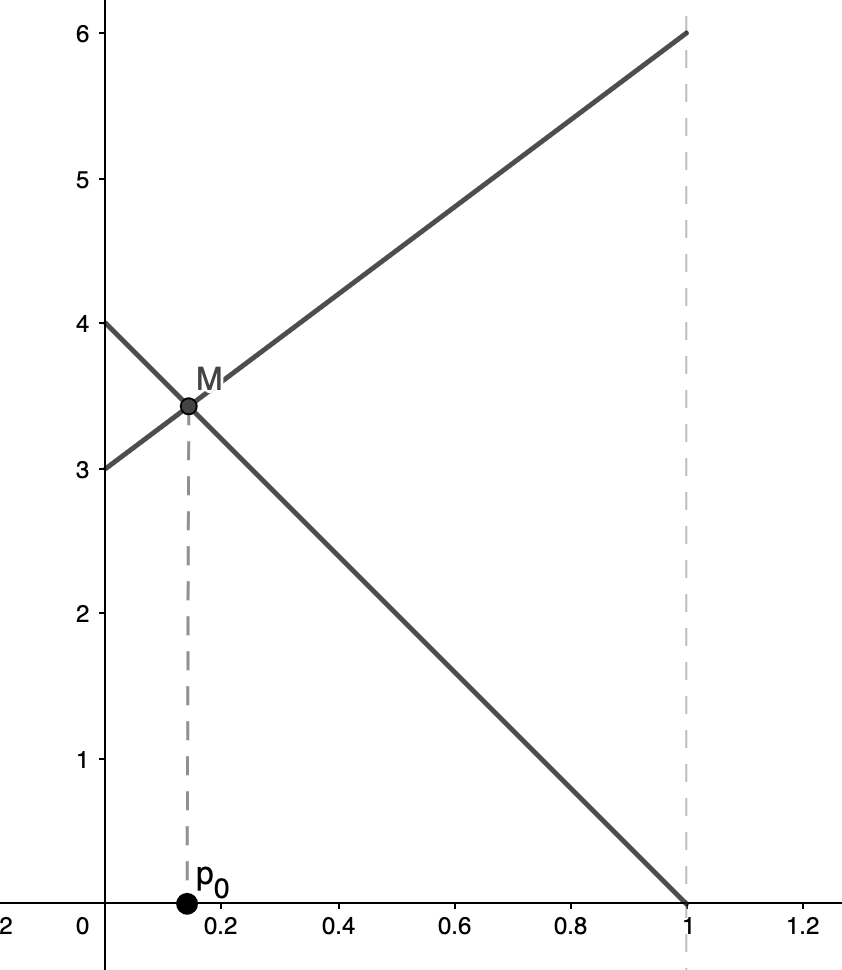
\includegraphics[width=0.3\columnwidth]{img/grafico1_es211028.png}
 \end{center}
 $$\begin{array}{c}
 3+3p_1 = 4+4p_1\\
 7p_1=1 \ \ p_1 = {1\over 2} \Rightarrow p_2 = {6\over 7}\\
 v^o = 3 + {3\over 7}= {24 \over 7}
 \end{array}$$
 \Sep
 \noindent
 \textcolor{blue}{Esempio 3:}
$$\begin{array}{c|ccc}
& \pi_1 & \pi_2 & \pi_3\\ \hline
p_1 & 0 & -2 & 2 \\
p_2 & 5 & 4 & -3 \\
\end{array}$$
$\begin{array}{c}
v'=0p_1+5(1-p_1)=5-5p_1\\
v''=-2p_1+4(1-p_1)=4-6_p1\\
v'''=2p_1-3(1-p_1) = -3 + 5p_1
\end{array}$
\begin{center}
 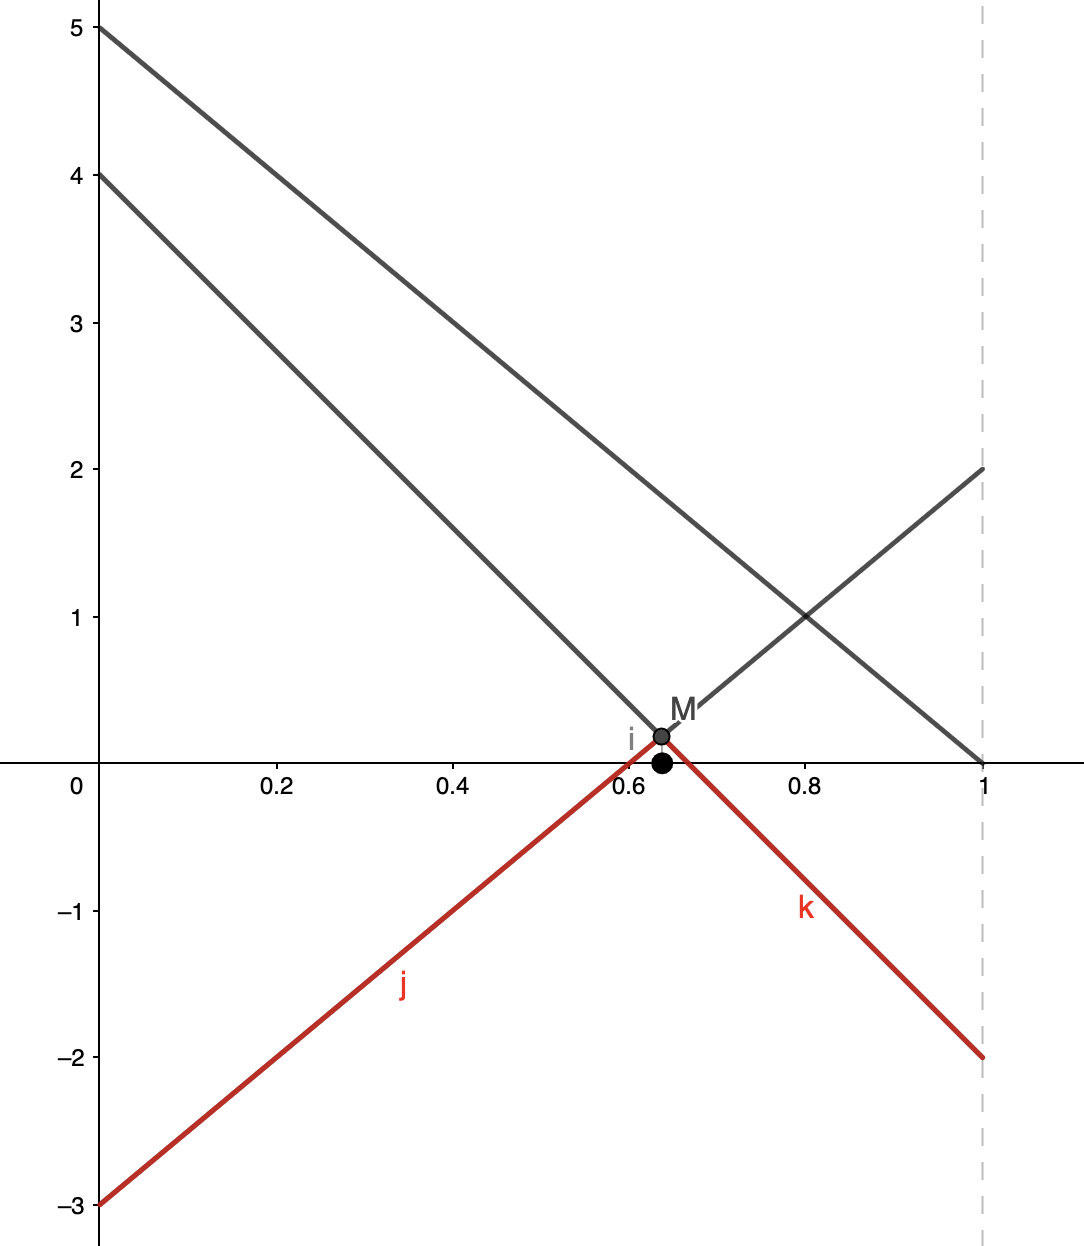
\includegraphics[width=0.3\columnwidth]{img/grafico2_es211028.png}
 \end{center}
 $$\begin{array}{c}
4-6p_1=-3+5p_1\\
11p_1 = 7 \ \ p_1 = {7 \over 11} \Rightarrow p_2 = {4\over 11}\\
v^o = 4 - {42 \over 11} = {2\over 11}
 \end{array}$$
 \Sep
 $$E[c_{ij}] = \sum_ip_i \sum_j \pi_j c_{ij} = \sum_i \sum_j p_i\pi_jc_{ij}$$
Dato che $\sum_j = \pi_j =1$ la minima vincita attesa sarà $min_j\sum_ip_i c_{ij} = v \Rightarrow$ lo risolvo come un problema di programmazione lineare cercando il $max \ v$
 $$\begin{array}{rl}
 max \ v & \\
  & \sum_ip_i =1\\
  & \sum_i p_i c_{ij} \geq v \ \ \forall j\\
  & p_i \geq 0 \ \ v \ libera\\
 \end{array} \ \ \ \ \begin{array}{c}
 m' + 1 \ \ \ \text{variabili}\\
 m'' + 1 \ \ \ \text{vincoli}
 \end{array}$$
 Riscritto in forma $max \ z = c^Tx$
  $$\begin{array}{rl}
 max \ v & \\
  & v - \sum_i p_i c_{ij} \leq 0 \ \ \forall j\\
  & \sum_ip_i =1\\
  & p_i \geq 0 \ \ v \ libera\\
 \end{array}\ \ 
 \begin{array}{c}
 \pi_j\\
 w
 \end{array}$$
 Scrivo il duale: ricordo che se $\begin{array}{rl}max & c^Tx \\
 & Ax \leq b\\
 & x \geq 0\\
 \end{array}$ allora il duale sarà $\begin{array}{rl}
 min & b^Ty\\
 & A^Ty \geq c\\
 & y \geq 0 \end{array}$: 
 $$\begin{array}{rlc}
 max \ v &  & \\
 & v-p_1c_{11}-p_2c_{21}-p_3c_{31} \leq 0 & \pi_1\\
 & v-p_1c_{12}-p_2c_{22}-p_3c_{32} \leq 0 & \pi_2\\
 & v-p_1c_{13}-p_2c_{23}-p_3c_{33} \leq 0 & \pi_3\\
 & v-p_1c_{14}-p_2c_{24}-p_3c_{34} \leq 0 & \pi_4\\
 & p_1+p_2+p_3+p_4 = 1 & w\\
 & p_1,p_2,p_3,p_4 \geq 0
 \end{array}$$
 Viene fuori che il duale è:
 $$\begin{array}{rl}
 min\ w & \\
 & - \sum_j\pi_j c_{ij} + w \leq 0\\
 & \pi_j \geq 0
 \end{array}$$
 La soluzione sarà che $w=max_i \sum_j \pi_j c_{ij}$
 
 %CAPITOLO
\clearpage
\section{08/11/2021 - Risolvere problemi di programmazione intera}
\subsection{Come risolvere un problema di programmazione intera?}
\textcolor{red}{Enumerazione}: Tutte le soluzioni possibili sono identificate e la migliore è
raccolta. Potrebbe non essere praticabile. Ad esempio, per risolvere il
Travelling Salesman Problem in un grafo completo con $n$ nodi ci sono $(n-1)!$ fattibili. Quindi,
$$\begin{array}{c|c}
n & n!\\
10 & 3.6 \times 10^6\\
100 & 9.33 \times 10^{157}\\
1000 & 4.02 \times 10^{2567}
\end{array}$$
Sono richieste idee migliori

\subsection{Il problema del mercante viaggiatore}
Ci viene dato un insieme di nodi $V=\{1,\dots,n\}$ (es. le città) e un insieme di archi $A$\\
Gli archi rappresentano coppie ordinate di città dove ci può essere un collegamento diretto.\\
Per $(i,j)\in A$ è il passaggio diretto dalla città $i$ alla città $j$\\
Gli obiettivi del TSP sono:
\begin{itemize}
\item Visitare tutte le città esattamente 1 volta, per poi tornare alla città di partenza
\item Impiegare il minor tempo di viaggio possibile
\end{itemize}
Un tour che visita tutti i nodi esattamente una volta si chiama \textcolor{red}{Hamiltonian tour}. Il TSP viene identificato come Hamiltonian tour di costo minimo.

\subsubsection{Un TSP facile}
 \begin{center}
 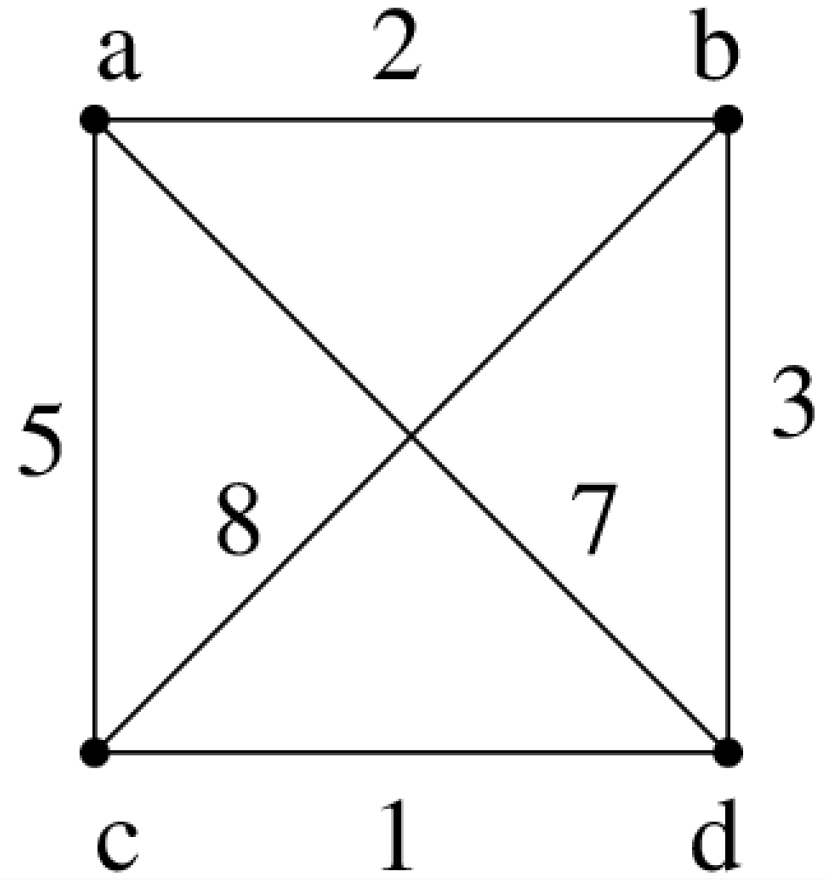
\includegraphics[width=0.4\columnwidth]{img/TSP_easy.png}
 \end{center}
Tre possibili Tour:
\begin{itemize}
\item \textcolor{red}{A-B-D-C-A - Costo: 11}
\item A-D-B-C-A - Costo: 23
\item A-D-C-B-A - Costo: 18
\end{itemize}

\subsubsection{Formulazione}
\textcolor{blue}{\textbf{Variabili decisionali}:} $$x_{ij} = \begin{cases}\begin{array}{ll}
1 & \text{se $j$ segue immediatamente $i$ nel tour}\\
0 & \text{altrimenti}
\end{array}
\end{cases}$$ Quindi $x \in \{0,1\}^{|A|}$
\textcolor{blue}{\textbf{Funzione obiettivo}:} $$min \sum_{(i,j)\in A}c_{ij}x_{ij}$$

\paragraph{Formulazione dei vincoli}
Ogni città viene inserita e lasciata una sola volta
$$\sum_{i:(i,j)\in A}x_{ij} = 1 \ \ \ per \ j \in V$$
$$\sum_{j:(i,j)\in A}x_{ij} = 1 \ \ \ per \ i \in V$$
Ma comunque i due vincoli appena citati non sono comunque abbastanza per definire i tour, dato che sono soddisfatti anche dai sotto-tour.
 \begin{center}
 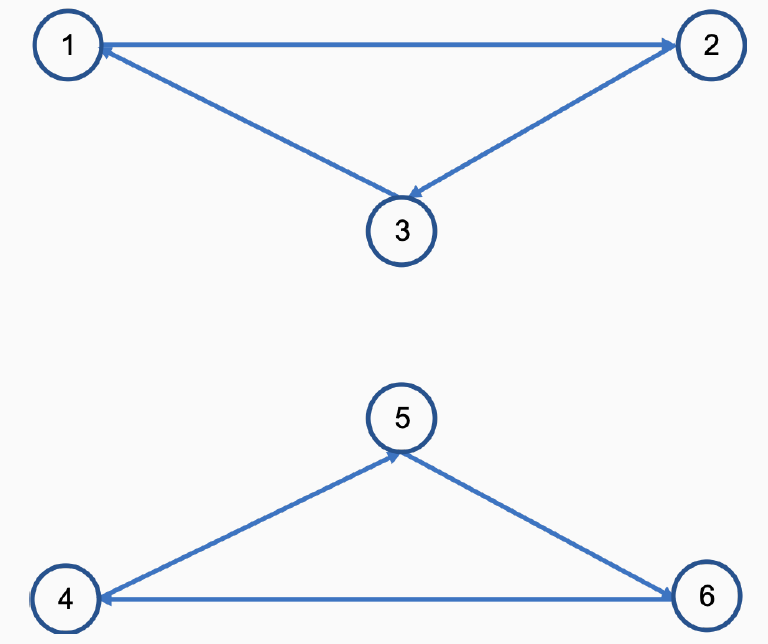
\includegraphics[width=0.4\columnwidth]{img/subtour1.png}
 \end{center}

\paragraph{Eliminazione dei sotto-tour}
In ogni tour ci deve essere un arco che va da $\{1,2,3\}$ a $\{4,5,6\}$ e un arco che va da $\{4,5,6\}$ a $\{1,2,3\}$. In generale, per ogni $U \subset V$ con $2 \leq |U| \leq |V|-2$, i vincoli 
$$\sum_{\{(i,j)\in A: i \in U, j \in V\backslash U}x_{ij} \geq 1$$
sono soddisfatti da tutti i tour, ma ogni sotto-tour ne viola almeno uno loro.
\begin{center}
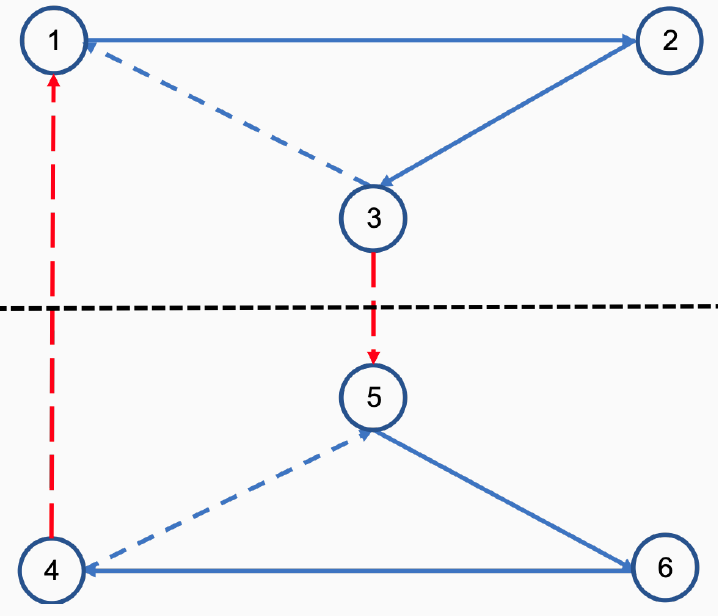
\includegraphics[width=0.4\columnwidth]{img/subtour2.png}
\end{center}
Un metodo alternativo per eliminare i sotto-tour è quelli di introdurre il vincolo
$$\sum_{\{(i,j)\in A: i \in U, j \in U}x_{ij} \leq |U|-1\ \forall U\subset V:2 \leq |U| \leq |V|-2$$
Ma anche in questo abbiamo bisogno di un vincolo per ogni $U\subset V$ tale che $2 \leq |U| \leq |V|-2$.\\
\\
In entrambi i casi il numero di vincoli è quasi $2^{|V|}$!
$${1\over 2}\left[\left(\begin{array}{c}|V| \\ 2\end{array}\right)+\left(\begin{array}{c}|V| \\ 3\end{array}\right) + \dots + \left(\begin{array}{c}|V| \\ |V|-2\end{array}\right)\right]$$

\Sep \Sep \noindent
\paragraph{Formulazione finale}
$$\begin{array}{rlr}
min\ z = & \sum_{(i,j) \in A}c_{ij}x_{ij} & \\
& \sum_{i:(i,j)\in A}x_{ij} = 1 & per \ j \in V\\
& \sum_{j:(i,j)\in A}x_{ij} = 1 & per \ i \in V\\
& \sum_{\{(i,j)\in A: i \in U, j \in V\backslash U}x_{ij} \geq 1 & \forall U\subset V:2 \leq |U| \leq |V|-2\\
& \textcolor{blue}{Oppure} & \\
& \sum_{\{(i,j)\in A: i \in U, j \in U}x_{ij} \leq |U|-1 & \forall U\subset V:2 \leq |U| \leq |V|-2\\
& x \in \{0,1\}^{|A|} &
\end{array}$$

\subsection{Come risolvere un problema intero?}
Ignorando i vincoli di integralità delle variabili. Consideriamo il problema che segue:
$$\begin{array}{rl}
max \ z = & 1,00 x_1 + 0,64 x_2\\
& 50 x_1 + 31 x_2 \leq 250\\
& 3 x_1 - 2x_2 \geq -4\\
& x_1,x_2  \in \N
\end{array}$$
La soluzione ottima intera è $(5,0)$\\
La soluzione ottima senza considerare le variabili di integrità dei vincoli è $\left({376\over193},{950\over193}\right)=(1.948,4.922)$
\begin{center}
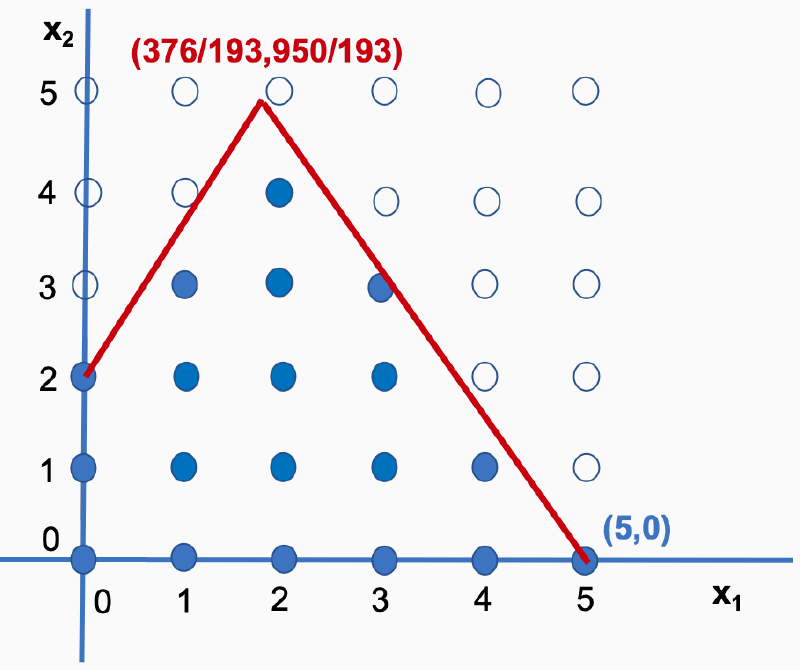
\includegraphics[width=0.4\columnwidth]{img/ip1.png}
\end{center}
Ignorando i vincoli di integralità delle variabili. Perché non arrotondare per eccesso e/o per difetto la soluzione lineare?
\begin{itemize}
\item La parte intera superiore $(2,5)$ non è ammissibile (Il primo vincolo viene violato)
\item La parte intera inferiore $(1,4)$ non è ammissibile (Il secondo vincolo viene violato)
\item La scelta mista $(1,5)$ non è ammissibile (Il secondo vincolo è violato)
\item La scelta mista $(2,4)$ è ammissibile ma non ottima, infatti notiamo che $z(2,4)=4.56$ e $z(5,0)=5$
\end{itemize}
Inoltre, nessun arrotondamento fornisce i valori $(5,0)$.
In conclusione, la soluzione lineare sembra essere inutile per trovare la soluzione intera.

\subsection{Ottimalità}
Dato un problema intero: $$z=max\{c(x):x\in X \subseteq \Z^n\}$$ come posso provare che un dato punto $x^*$ è ottimo?\\
Dobbiamo rispondere a questa domanda perché abbiamo visto che la soluzione dell'enumerazione potrebbe non essere possibile, mentre ignorando le variabili i vincoli di integralità potrebbero non fornire informazioni utili.\\
Quindi abbiamo bisogno di trovare degli algoritmi per risolvere un problema intero.

\subsection{Limiti}
L'approccio più comune per risolvere un problema intero è quello di trovare delle sequenze di limiti finché non sono "abbastanza chiusi". Definisco quindi\\
\textbf{Limite superiore (Upper Bound)}: Se $z$ è la soluzione ottima di un problema intero, un limite superiore è un valore $\overline{z}$ tale che $\overline{z} \geq z$.\\
\textbf{Limite inferiore (Lower Bound)}: Se $z$ è la soluzione ottima di un problema intero, un limite inferiore è un valore $\underline{z}$ tale che $\underline{z} \leq z$.\\
Idealmente vogliamo trovare quei $\overline{z}$ e $\underline{z}$ tali che $\underline{z} = z = \overline{z}$\\
\\
Da un punto di vista più pratico, ogni algoritmo andrà a cercare una sequenza decrescente di limiti superiori
$$\overline{z_1} > \overline{z_2} > \dots > \overline{z_s} \geq z$$
e una sequenza crescente di limiti inferiori
$$\underline{z_1} < \underline{z_2} < \dots < \underline{z_t} \leq z$$
e si stoppa quando $$\overline{z_s} - \underline{z_t} \leq \epsilon$$
dove $\epsilon$ è un valore non negativo appropriato.

\subsubsection{Limite inferiore}
\textbf{Def.}: Ogni soluzione ammissibile $\hat x \in X$ fornisce un limite inferiore (o primale) $\underline{z}=c(\hat x) \leq z$\\
Per il problema $$\begin{array}{rl}
max \ z = & 1,00 x_1 + 0,64 x_2\\
& 50 x_1 + 31 x_2 \leq 250\\
& 3 x_1 - 2x_2 \geq -4\\
& x_1,x_2  \in \N
\end{array}$$
vediamo, arrotondando la soluzione ottima, che $\hat x =(2,4)$ è una soluzione ammissibile tale $\underline{z}=c(\hat x)=4.56 \leq z$

\subsubsection{Limite superiore}
I limiti superiori dei risultati potrebbero essere meno ovvi.\\
L'idea più comune è quella di sostituire un problema intero "difficile" con un problema di ottimizzazione più semplice, il cui valore ottimo è almeno grande quanto $z$.\\
Il problema più semplice può essere ottenuto per "rilassamento", cioè, da
\begin{itemize}
\item Allargando l'insieme delle soluzioni ammissibili in modo da ottimizzare su un insieme più grande
\item Sostituendo la funzione obiettivo $max$ con una funzione che abbia lo stesso o un valore maggiore ovunque.
\end{itemize}

\subsection{Rilassamento}
\textcolor{blue}{\textbf{Definizione}:} Un problema (rilassato) $z^R=max\{f(x):x\in T\subseteq \R^n\}$ è il rilassamento di un problema intero $z=max\{c(x):x\in X \subseteq \Z^n\}$ se: \begin{itemize}
\item[i.] $X\subseteq T$
\item[ii.] $f(x) \geq c(x)$ per tutte le $x \in X$
\end{itemize}
\textbf{Proposizione, se RP è il rilassamento di IP, $z^R \geq z$}: Se $x^*$ è una soluzione ottima del problema intero, $x^*\in X \subseteq T$ e $z=c(x^*) \leq f(x^*)$. $x^* \in T, f(x^*)$ è un limite inferiore su $z^R$, quindi $z\leq f(x^*) \leq z^R$.\\
Quindi $z^R$ è un limite superiore.

\subsection{Rilassamento lineare}
\textcolor{blue}{\textbf{Definizione}:} Per un programma intero $max\{cx:c\in X = P \cap \Z^n\}$ con una formulazione $P=\{x \in \R_+^n:Ax\leq b\}$, il \textcolor{red}{problema lineare rilassato} è il problema lineare $z^{LP}=max\{cx:x\in P\}$\\
\\
Poiché $X=P\cap\Z^n \subseteq P$ e la funzione obiettivo sono invariati, questo è chiaramente un rilassamento.

\subsubsection{Esempio}
\begin{Parallel}{0.45 \textwidth}{0.45 \textwidth}
   \ParallelLText{\textbf{Problema intero originale}
  $$\begin{array}{rl}
  z = max & 1,00 x_1 + 0,64 x_2\\
  & 50 x_1 + 31 x_2 \leq 250\\
  & 3 x_1 - 2x_2 \geq -4\\
  & x_1,x_2  \in \N
  \end{array}$$}
   \ParallelRText{\textbf{Rilassamento lineare}
   $$\begin{array}{rl}
  z^{LP} = max& 1,00 x_1 + 0,64 x_2\\
  & 50 x_1 + 31 x_2 \leq 250\\
  & 3 x_1 - 2x_2 \geq -4\\
  & x_1,x_2 \geq 0
  \end{array}$$}
\end{Parallel}
\begin{itemize}
\item La soluzione ottima intera è $(5,0)$ e $z=5$
\item La soluzione ottima del rilassamento lineare è $\left({376 \over 193}, {950\over 193}\right)$ e $z^{LP} = {984 \over 193} = 5,098$
\end{itemize}
\begin{center}
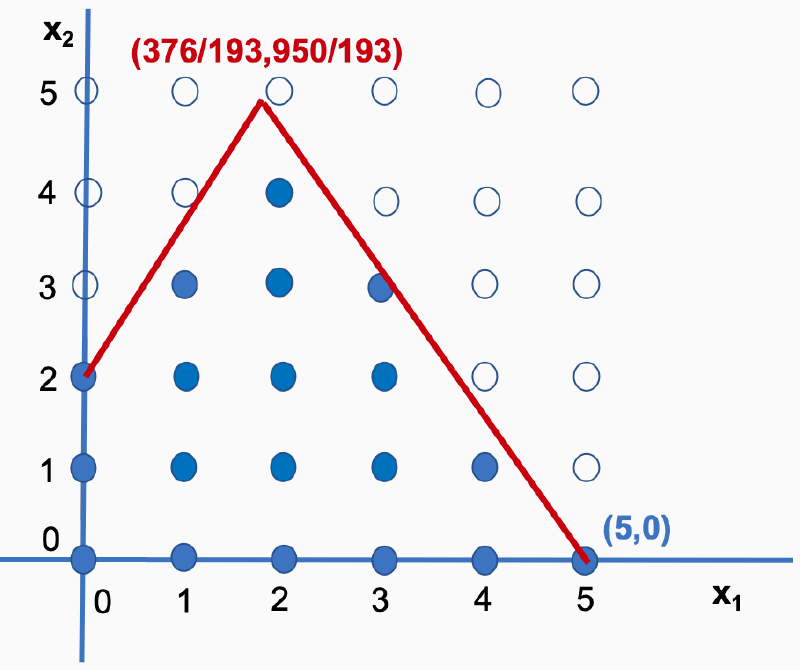
\includegraphics[width=0.4\columnwidth]{img/ip1.png}
\end{center}
Per il problema intero
$$\begin{array}{rl}
  z = max & 1,00 x_1 + 0,64 x_2\\
  & 50 x_1 + 31 x_2 \leq 250\\
  & 3 x_1 - 2x_2 \geq -4\\
  & x_1,x_2  \in \N
  \end{array}$$
Sappiamo che il limite inferiore è $\underline{z}=4,560$ e il limite superiore è $\overline{z}=5,098$. La soluzione ottima $z$ si trova quindi all'interno di $$\underline{z}=4,560 \leq z \leq 5,098 = \overline{z}$$
Infatti, $z=5$.\\
Le informazioni che otteniamo ignorando le variabili i vincoli di integralità possono essere davvero molto utili.
 
%CAPITOLO
\clearpage 
\section{09/11/2021 - Problemi ben posti}
\subsection{Impostare il contesto}
Un punto di partenza naturale nella risoluzione di programmi interi lineari $$(IP) \ \ max\{cx:Ax \leq b, x \in Z^n\}$$ con dati integrali $(A, b)$ è chiedersi quando si sarà così fortunati che il rilassamento della programmazione lineare $$(LP) \ \ max\{cx:Ax \leq b, x\in \R^n\}$$ avrà una soluzione ottima integrale.

\subsection{Unimodularità totale}
\textbf{Def.}: Una matrice $A$ è totalmente unimodulare (TU) se ogni sotto matrice quadrata di $A$ ha determinante $+1$, $-1$ o $0$\\
\textbf{Osservazione}: Se $A$ è TU, $a_{ij}\in\{+1,-1,0\}$\\
Matrici non TU
   $$A_1 = \left(\begin{array}{cc}1&-1\\1&1\end{array}\right) \ \ \ \ |A_1|=2$$
   $$A_2 = \left(\begin{array}{ccc}1&1&0\\0&1&1\\1&0&1\end{array}\right) \ \ \ \ |A_2|=2$$
Matrice TU
   $$A_3 = \left(\begin{array}{cccc}
   1 & -1 & -1 & 0\\
   -1 & 0 & 0 & 1\\
   0 & 1 & 0 & -1\\
   0 & 0 & 1 & 0
   \end{array}\right) \ \ \ \ |A_3| = 0$$

\subsection{Proposizione 1}
Una matrice $A$ è TU se e solo se\begin{itemize}
\item La matrice trasposta $A^T$ è TU
\item La matrice $[A|I]$ è TU
\end{itemize}

\subsection{Proposizione 2 - Condizione sufficiente}
Una matrice è TU se \begin{itemize}
\item[i.] $a_{ij}\in \{+1,-1,0\}$
\item[ii.] Ogni colonna contiene al massimo due coefficienti diversi da zero, cioè $\sum_i |a_{ij}| \leq 2$
\item[iii.] Esiste una partizione ($M_1,M_2$) delle $M$ righe tale che ciascuna colonna $j$ contenente due coefficienti diversi da zero soddisfa $$\sum_{i \in M_1}a_{ij} - \sum_{i\in M_2}a_{ij}=0$$
\end{itemize}
La condizione (iii) significa che se $i$ non ha zeri nella riga $i$ e $k$, e se $a_{ij} = -a_{kj}$, allora $\{i, k\} \in M_1$ o $\{i, k\} \in M_2$, mentre se $a_{ij} = a_{kj} ,\ i \in M_1$ e $k \in M_2$ o viceversa.

\subsection{Proposizione 3}
Il problema di programmazione lineare $max\{cx : Ax \leq b,\ x \in R^n_+\}$ ha una soluzione ottima intera per tutti i vettori interi $b$ per i quali ha valore ottimo finito se e solo se $A$ è totalmente unimodulare.

\subsection{Minimum cost network flow}
Dato un grafo $D = (V,A)$ con capacità d'arco $h_{ij}$ per ogni $(i, j) \in A$, richiede $b_i$ (afflussi positivi o deflussi negativi) ad ogni nodo $i \in V$, e il costo del flusso unitario $c_{ij}$ per tutti $(i, j) \in A$. Il problema del flusso di rete di costo minimo è trovare un flusso fattibile che soddisfi tutte le esigenze al minimo costo. Questo ha il formulazione
$$min\sum_{(i,j)\in A} c_{ij}x_{ij} \ \ \ \ (1)$$
$$\sum_{k\in V^+(i)}x_{ik} - \sum_{k \in V^-(i)}x_{ki} = b_i \ per\ i \in V \ \ \ \ (2)$$
$$0\leq x_{ij} \leq h_{ij} \ per \ (i,j)\in A \ \ \ \ (3)$$
dove $x_{ij}$ denota il flusso in arco $(i,j), V^+(i)=\{k:(i,k)\in A\}$ e $V^-(i)=\{k:(k,1) \in A\}$
\begin{center}
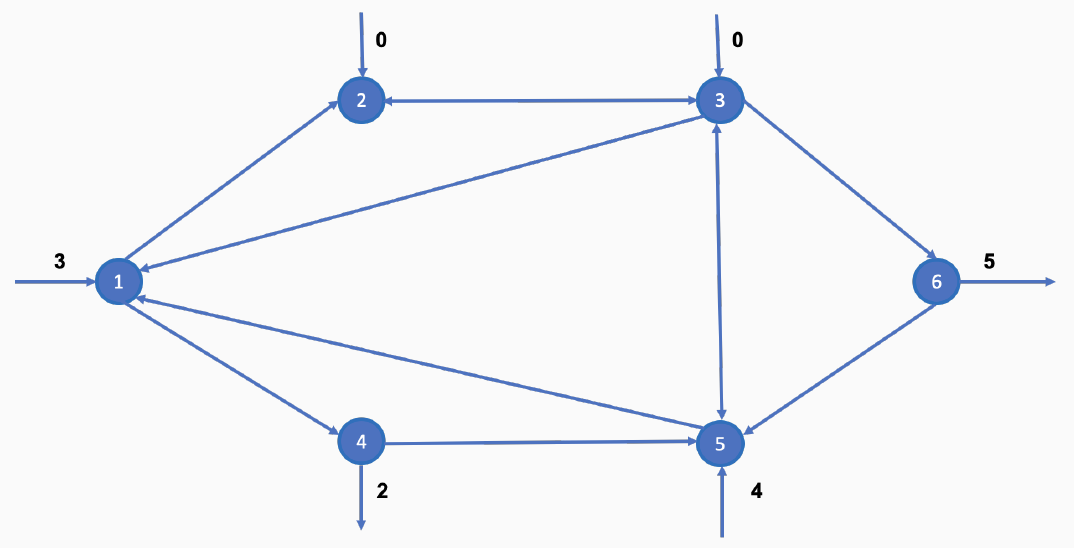
\includegraphics[width=0.5\columnwidth]{img/fcm.png}
\end{center}
\begin{equation*}
\begin{array}{ccccccccccccc}
x_{12} & x_{14} & x_{23} & x_{31} & x_{32} & x_{35} & x_{36} & x_{45} & x_{51} & x_{53} & x_{65} & &\\ \hline
1 & 1 & 0 & -1 & 0 & 0 & 0 & 0 & -1 & 0 & 0 & = & 3\\
-1 & 0 & 1 & 0 & -1 & 0 & 0 & 0 & 0 & 0 & 0 & = & 0\\
0 & 0 & -1 & 1 & 1 & 1 & 1 & 0 & 0 & -1 & 0 & = & 0\\
0 & -1 & 0 & 0 & 0 & 0 & 0 & -1 & 0 & 0 & 0 & = & -2\\
0 & 0 & 0 & 0 & 0 & -1 & 0 & -1 & 1 & 1 & -1 & = & 4\\
0 & 0 & 0 & 0 & 0 & 0 & -1 & 0 & 0 & 0 & 1 & = & -5\\
\hline
\end{array}
\end{equation*}
I vincoli aggiuntivi sono i vincoli di capacità $0 \leq x_{ij} \leq h_{ij}$

\subsection{Proposizione 4}
La matrice dei vincoli $A$ derivante da un flusso di rete di un problema di costo minimo è totalmente unimodulare.\\
\\
\textbf{Dim.}: La matrice A è della forma $\left(\begin{array}{c}C\\I\end{array}\right)$ dove $C$ viene da vincoli di conservazione del flusso e $I$ dai vincoli di capacità. Quindi basta mostrare che $C$ è TU. Le condizioni sufficienti affinché la Proposizione 2 sia soddisfatta sono $M_1 = M$ e $M_2 = \emptyset$.

\subsection{Risultato chiave - Corollario}
In un problema di flusso di rete di costo minimo, se le richieste $\{b_i\}$ e le capacità $\{h_{ij}\}$ sono integrali
\begin{itemize}
\item Ogni punto estremo è integrale
\item I vincoli (2) e (3) descrivono l'inviluppo convesso dei flussi integrali ammissibili.
\end{itemize}

\SmallSep\noindent
Questo corollario significa che il rilassamento lineare del problema del flusso di rete di costo minimo fornisce sempre una soluzione intera fornita che tutte le capacità $\{h_{ij}\}$ e le richieste $\{b_i\}$ sono integrali.

\subsection{Flussi speciali a costo minimo}
\subsubsection{Il problema del percorso più breve}
Dato un grafo $D = (V,A)$, due nodi distinti $s, t \in V$, e gli archi non negativi costano $c_{ij}$ per $(i, j) \in A$, trova un costo minimo sul percorso $s-t$.\\
\\
Se poniamo $b_s = 1$ e $b_t = -1$, solo un'unità di flusso può spostarsi da $s$ a $t$, e il problema è trovare la successione degli archi a costo minimo che questa unità attraverserà. Un arco $(i, j) \in A$ se e solo se $h_{ij} > 0$. Poiché assumiamo solo valori interi, $(i, j) \in A$ se e solo se $h_{ij} \geq 1$. Poiché nella rete scorre esattamente un'unità, non è necessario
includere esplicitamente i vincoli di capacità.\\
Le variabili decisionali sono tali che $x_{ij} = 1$ se $arc(i, j)$ è al minimo costo (più breve) il percorso $s-t$. Per l'unimodularità totale, una soluzione ottima è sempre intera. Pertanto, possiamo scrivere $x_{ij} \geq 0$.

\paragraph{Esempio}
\begin{center}
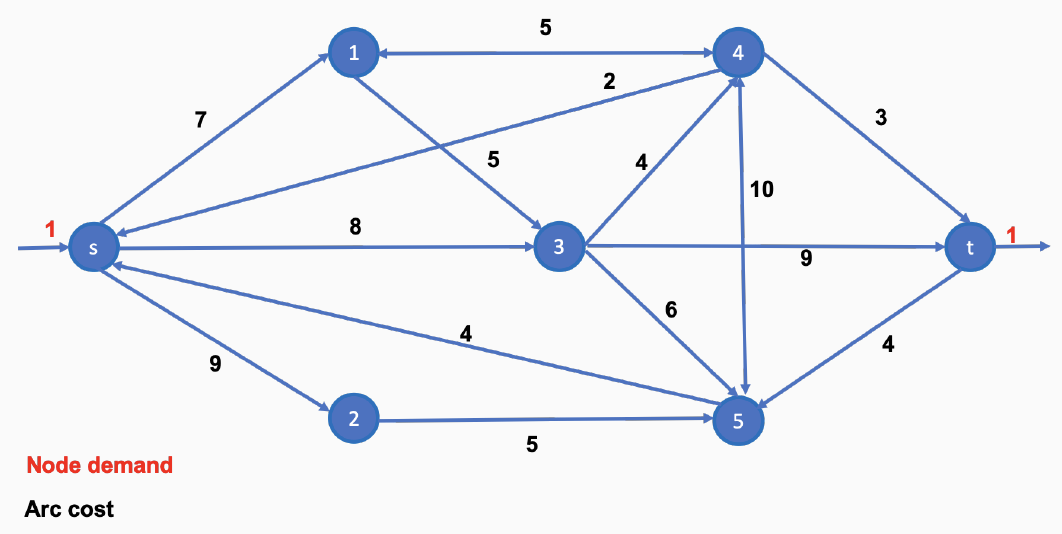
\includegraphics[width=0.5\columnwidth]{img/fcm2.png}
\end{center}
$$\begin{array}{rll}
z = & min \sum_{(i,j)\in A}c_{ij}x_{ij} &\\
& \sum_{k \in V^+(i)}x_{ik} - \sum_{k\in V^-(i)}x_{ki}=1 & per\ i=s\\
& \sum_{k \in V^+(i)}x_{ik} - \sum_{k\in V^-(i)}x_{ki}=1 & per\ i\in V \setminus \{s,t\}\\
& \sum_{k \in V^+(i)}x_{ik} - \sum_{k\in V^-(i)}x_{ki}=-1 & per\ i=t\\
& x_{ij} \geq 0 & per\ (i,j) \in A
\end{array}$$

\subsubsection{Il problema del percorso più lungo}
Dato un grafo $D = (V,A)$, due nodi distinti $s, t \in V$, e capacità non negative $h_{ij}$ per $(i, j) \in A$, trovare un flusso massimo sul percorso da $s$ a $t$.\\
\\
Sommando un arco all'indietro da $t$ a $s$, il problema di flusso massimo $s - t$ può essere formulato come
$$\begin{array}{rll}
z = & max x_{ts} &\\
& \sum_{k \in V^+(i)}x_{ik} - \sum_{k\in V^-(i)}x_{ki}=0 & per\ i\in V\\
& 0 \leq x_{ij} \leq h_{ij} & per\ (i,j) \in A
\end{array}$$
Per l'unimodularità totale, una soluzione ottima è fornita intera che tutte le capacità $h_{ij}$ sono integrali.
\begin{center}
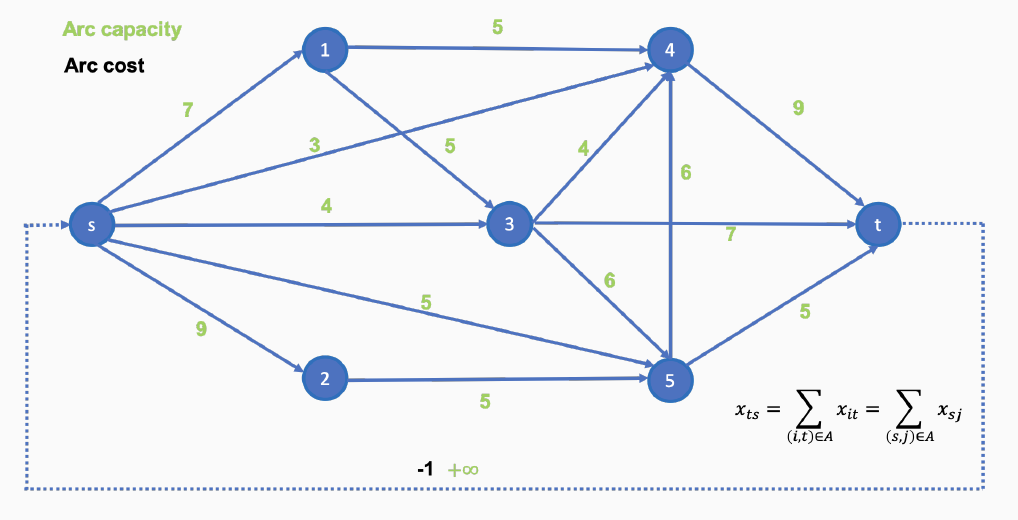
\includegraphics[width=0.5\columnwidth]{img/fcmax.png}
\end{center}

\subsubsection{Problema di trasporto}
Siano $m$ fornitori e $n$ consumatori. l'$i-esimo$ fornitore può fornire $a_i$ unità di un certo bene e il $j-esimo$ consumatore domanda $b_j$ unità. Se $c_{ij}$ è il costo per trasportare un'unità di bene dall'$i-esimo$ fornitore al $j-esimo$ consumatore, il problema è trasportare la merce dal fornitori ai consumatori al minimo costo.\\
\\
Può essere formulato come un problema di flusso di costo minimo su un grafo bipartito $D = (V_1 \cup V_2,A)$ dove $V_1 = \{1, \dots ,m\}$ è l'insieme delle sorgenti, $V_2 = \{1, \dots , n\}$ è l'insieme delle destinazioni, e $A = \{(i, j) :\ i \in V_1,\ j \in V2\}$. Senza perdita di generalità, assumiamo che ci sia un arco da ciascun nodo di offerta a ciascun nodo di domanda. Il costo di spedizione unitario da $i \in V_1$ a $j\in V_2$ è $c_{ij}$ . Se non c'è un arco da $i$ a $j$, prendiamo $c_{ij}$ molto grande. Il nodo $i \in V_1$ ha un'alimentazione positiva $a_i$ e $j \in V_2$ ha a domanda positiva $b_j$. Il flusso in uscita da una sorgente è necessario per uguagliare la sua offerta e il flusso delle destinazioni deve essere uguale alla sua domanda.\\
Quindi una condizione necessaria per la fattibilità è 
$$\sum_{i\in V_1}a_i = \sum_{j\in V_2}b_j$$
$$\begin{array}{rll}
z = & min \sum_{i\in V_1}\sum_{i \in V_2} c_{ij}x_{ij} &\\
& \sum_{j \in V_2}x_{ij} = a_i & per\ i\in V_1\\
& \sum_{i \in V_1}x_{ij} = b_j & per\ j\in V_2\\
& x_{ij} \geq 0 & per\ (i,j) \in A
\end{array}$$
\begin{center}
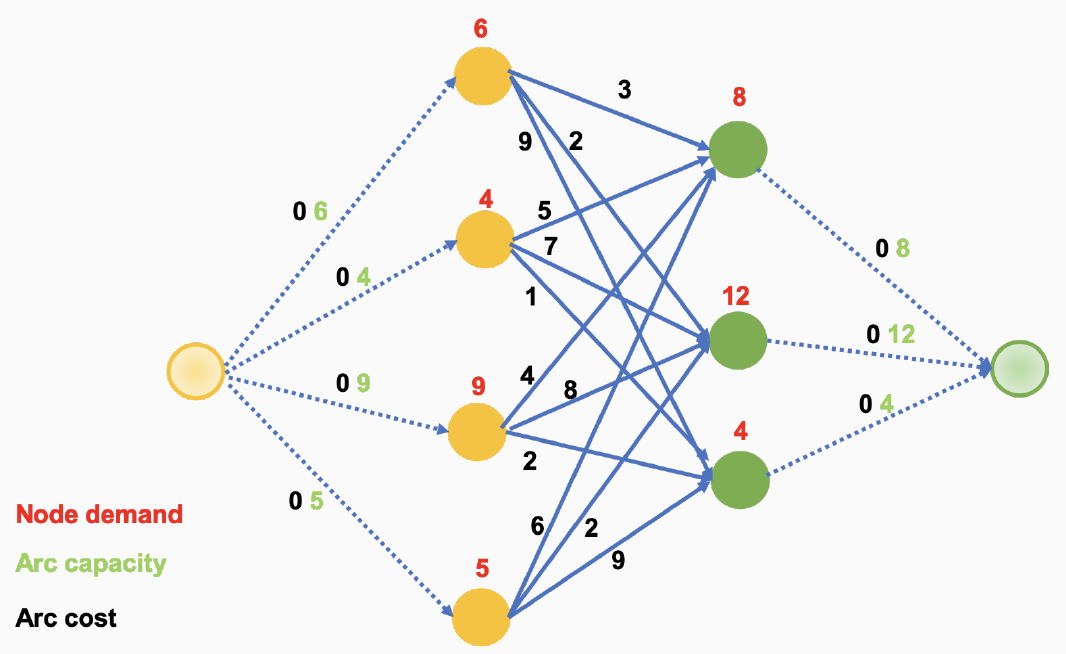
\includegraphics[width=0.5\columnwidth]{img/tp.png}
\end{center}

\subsubsection{Problema dell'assegnazione} 
\'E un caso speciale del problema del trasporto, dove il numero dei fornitori è uguale al numero dei consumatori, ogni fornitore ha l'offerta unitaria e ogni consumatore ha la domanda unitaria.\\\\
Quando $a_i=b_j=1$ per tutti gli $i$ e $j$ e $m=n$, abbiamo il problema dell'assegnazione
$$\begin{array}{rll}
z = & min \sum_{i\in V_1}\sum_{i \in V_2} c_{ij}x_{ij} &\\
& \sum_{j \in V_2}x_{ij} = 1 & per\ i\in V_1\\
& \sum_{i \in V_1}x_{ij} = 1 & per\ j\in V_2\\
& 0 \leq x_{ij} \leq 1 & per\ (i,j) \in A
\end{array}$$
\begin{center}
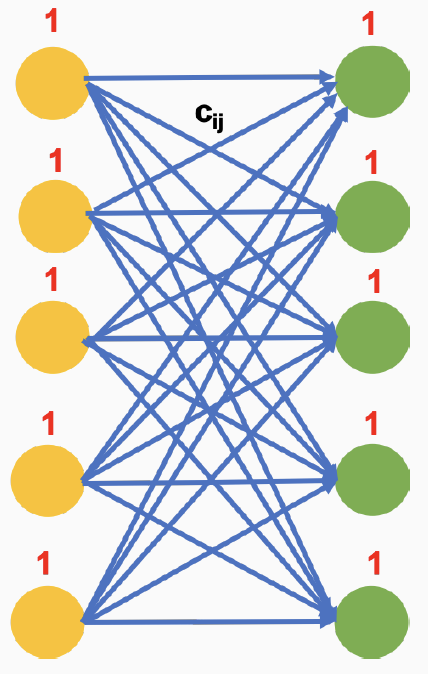
\includegraphics[width=0.4\columnwidth]{img/ap.png}
\end{center}
Supponiamo che ci siano $n$ persone e $m$ lavori, dove $n \geq m$. Ogni lavoro deve essere fatto esattamente da una persona; inoltre, ogni persona può fare, al massimo, un lavoro. Il costo della persona $j$ che fa il lavoro $i$ è $c_{ij}$ . Il problema è assegnare le persone ai lavori in modo da ridurre al minimo il costo totale di completando tutti i lavori. Per formulare questo problema, che è noto come problema di assegnazione, introduciamo $0-1$ variabili $x_{ij} ,\ i = 1, \dots , m,\  j = 1, \dots , n$ corrispondente all'$ij-esimo$ evento di assegnare la persona $j$ al lavoro $i$.\\
Poiché esattamente una persona deve svolgere il lavoro i, abbiamo dei vincoli
$$\sum_{j=1}^nx_{ij} = 1\ \  per\ i=1,\dots,m \ \ \ \ (4)$$
Poiché ogni persona non può svolgere più di un lavoro, abbiamo anche dei vincoli
$$\sum_{i=1}^m x_{ij} \leq 1 \ \ per\ j=1,\dots,n \ \ \ \ (5)$$
È ora facile verificare che se $x \in \{0, 1\}^{mn}$ soddisfa (4) e (5), si ottiene un soluzione praticabile del problema di assegnazione. La funzione obiettivo è
$$min\sum_{i=1}^m\sum_{j=1}^n x_{ij}x_{ij}$$

\paragraph{Esempio}: Un'azienda ha a disposizione 4 macchine per l'assegnazione di 4 attività. Qualunque macchina può essere assegnata a qualsiasi attività e ogni attività richiede
elaborazione da parte di una macchina. Il tempo necessario per configurare ciascuna
macchina per l'elaborazione di ciascuna attività è riportata nella tabella sottostante.
\begin{center}
\begin{tabular}{ccccc}
& A1 & A2 & A3 & A4 \\ \hline
M1 & 13 & 4 & 7 & 6 \\
M2 & 1 & 11 & 5 & 4 \\
M3 & 6 & 7 & 2 & 8 \\
M4 & 1 & 3 & 5 & 9 \\ \hline
\end{tabular}
\end{center}
L'azienda vuole ridurre al minimo il tempo totale di installazione necessario per l'elaborazione di tutte e quattro le attività.\\
Se pensiamo ai tempi di setup come costi e definiamo
\begin{equation*}
x_{ij} = \begin{cases}
\begin{array}{ll}
1 & \text{se la macchina $i$ è assegnata al processo $j$}\\
0 & \text{se la macchina $i$ non è assegnata al processo $j$}
\end{array}
\end{cases}
\end{equation*}
dove $i = 1, 2, 3, 4$ e $j = 1, 2, 3, 4$, allora si vede facilmente che cosa abbiamo un problema con 4 sorgenti (che rappresentano le macchine), 4 destinazioni (che rappresentano i compiti), una singola unità di fornitura da ciascuno sorgente (che rappresenta la disponibilità di una macchina) e una singola unità della domanda ad ogni destinazione (che rappresenta il requisito di elaborazione di un compito). Questa particolare classe di problemi è chiamata problemi di assegnamento.
\begin{center}
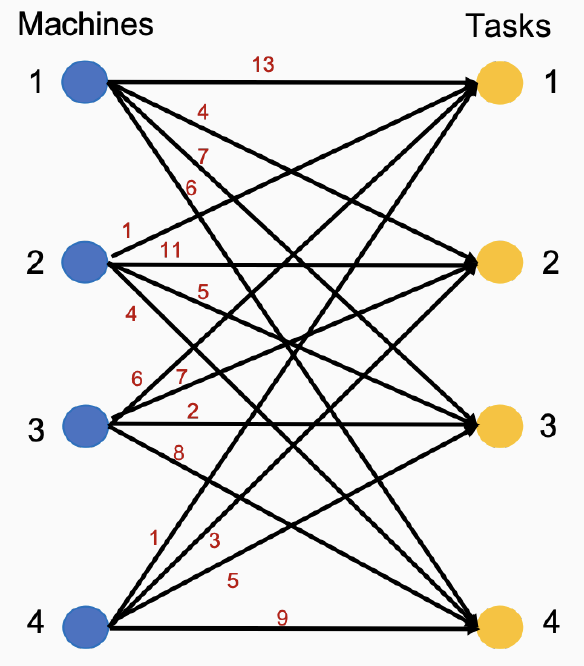
\includegraphics[width=0.4\columnwidth]{img/es_ap.png}
\end{center}
\begin{equation*}
\begin{array}{rl}
min & 13x_{11} + 4x_{12} + 7x_{13}+6x_{14}+\\
&x_{21} + 11x_{22} + 5x_{23}+4x_{24} +\\
&6x_{31} + 7x_{32} + 2x_{33}+8x_{34}+\\
&x_{41} + 3x_{42} + 5x_{43}+9x_{44}\\
\end{array}
\end{equation*}
\SmallSep
\begin{equation*}
\begin{array}{l}
x_{11} + x_{12} + x_{13} + x_{14} = 1\\
x_{21} + x_{22} + x_{23} + x_{24} = 1\\
x_{31} + x_{32} + x_{33} + x_{34} = 1\\
x_{41} + x_{42} + x_{43} + x_{44} = 1\\
\end{array}
\end{equation*}
\SmallSep
\begin{equation*}
\begin{array}{l}
x_{11} + x_{21} + x_{31} + x_{41} = 1\\
x_{12} + x_{22} + x_{32} + x_{41} = 1\\
x_{13} + x_{23} + x_{33} + x_{43} = 1\\
x_{14} + x_{24} + x_{34} + x_{44} = 1\\
\end{array}
\end{equation*}
$$x_{ij} \in \{0,1\}, \ per\ i=1,\dots, 4, \ j=1,\dots,4$$

%CAPITOLO
\clearpage
\section{25/11/2021 - Condizioni KKT}
\begin{enumerate}
\item ${\partial f \over \partial x_i} - \sum_{i}^m\lambda_i {\partial g_i \over \partial x_j} \leq 0 \ \ \ \forall j$
\item $v_j \left[{\partial f \over \partial x_i} - \sum_{i}^m\lambda_i {\partial g_i \over \partial x_j}\right] = 0 \ \ \ \forall j$
\item $\lambda_i \left[g_i(x) - b_i\right] = 0 \ \ \ \forall i$
\item $g_i(x) - b_i \leq 0 \ \ \ \forall i$
\item $x_j \geq 0$
\item $\lambda_i \geq 0$
\end{enumerate}

\subsection{Esercizio 1 - Facile}
\begin{equation*}
\begin{array}{rl}
max \ f(x) = & log(x_1+1)+x_2\\
& 2x_1+x_2 \leq 3\\
& x_1,\ x_2 \geq 0
\end{array}
\end{equation*}

\begin{enumerate}
\item \begin{enumerate}
\item[1] ${1 \over x_1 +1} - 2\lambda \leq 0$
\item[2] $1-\lambda \leq 0$\end{enumerate}
\item \begin{enumerate}
\item[1] $x_1 \left({1 \over x_1 +1} - 2\lambda\right) = 0$
\item[2] $x_2(1-\lambda)=0$
\end{enumerate}
\item $\lambda(2x_1+x_2-3) = 0$
\item $2x_1+x_2 - 3 \leq 0$
\item $x_1,\ x_2 \geq 0$
\item $\lambda \geq 0$
\end{enumerate}

\SmallSep \noindent
Dalla $1.2$ so che $\lambda \geq 1 \Rightarrow {1 \over x_1 +1} - 2\lambda \not = 0 $ 
$$\begin{array}{rll}
 (2.1) & & \Rightarrow\ x_1 = 0\\
 (3) & \Rightarrow\ 2x_1+x_2-3 = 0 & \Rightarrow x_2 = 3\\
 (2.2) & \Rightarrow\ x_2(1-\lambda)=0 & \Rightarrow \lambda= 1
\end{array}$$

\subsection{Esercizio 2 - Medio}
\begin{equation*}
\begin{array}{rl}
max \ f(x) = & x_1+2x_2-x_2^3\\
& x_1+x_2 \leq 1\\
& x_1,\ x_2 \geq 0
\end{array}
\end{equation*}

\begin{enumerate}
\item \begin{enumerate}
\item[1] $1 - \lambda \leq 0$
\item[2] $2-3x_2^2 - \lambda \leq 1$\end{enumerate}
\item \begin{enumerate}
\item[1] $x_1(1-\lambda) = 0$
\item[2] $x_2(2-3x_2^2 - \lambda)=0$
\end{enumerate}
\item $\lambda(x_1+x_2-1) = 0$
\item $x_1+x_2-1 \leq 0$
\item $x_1,\ x_2 \geq 0$
\item $\lambda \geq 0$
\end{enumerate}

\SmallSep \noindent
Dalla $1.1$ so che $\lambda \geq 0$ quindi per la $3$ $x_1+x_2 =1$\\
Suddivido l'esercizio in due casi:
\begin{itemize}
\item Sia $x_1 > 0$.\\
Dalla $2.1$ ottengo $\lambda=1$\\
Dalla $1.2$ trovo che $3x_2^2 \geq 1 \Rightarrow x_2 \geq +\sqrt{1\over 3}$\\
Per trovare il valore di $x_1$ utilizzo la $2.2$ e trovo che $x_1 = 1-{1\over \sqrt{3}}$
\item Sia $x_1 = 0$.\\
Ottengo che $x_2 =1$ e dalla $2.2$ che $\lambda = -1$ il che non è ammissibile
\end{itemize}

\subsection{Esercizio 3 - Difficile}
\begin{equation*}
\begin{array}{rl}
max \ f(x) = & 20x_1+10x_2\\
& x_1^2 + x_2^2 \leq 1\\
& x_1 + 2x_2 \leq 2\\
& x_1,\ x_2 \geq 0
\end{array}
\end{equation*}

\begin{enumerate}
\item \begin{enumerate}
\item[1] $20 -\lambda_12x_1 - \lambda_2 \leq 0$
\item[2] $10 - \lambda_12x_2 - \lambda_2 \leq 0$\end{enumerate}
\item \begin{enumerate}
\item[1] $x_1(20 -\lambda_12x_1 - \lambda_2) = 0$
\item[2] $x_2(10 -\lambda_12x_1 - \lambda_2)=0$
\end{enumerate}
\item \begin{enumerate}
\item[1] $\lambda_1(x_1^2 + x_2^2 - 1) = 0$
\item[2] $\lambda_2(x_1+2x_2-2) =0$
\end{enumerate}
\item \begin{enumerate}
\item[1] $x_1^2 + x_2^2 - 1\leq 0$
\item[2] $x_1+2x_2-2 \leq 0$
\end{enumerate}
\item $x_1,\ x_2 \geq 0$
\item $\lambda \geq 0$
\end{enumerate}

\SmallSep \noindent
Per trovare la risoluzione di questo esercizio devo andare ad analizzare diversi casi:
\begin{itemize}
\item Sia $\lambda_1=\lambda_2=0$.\\
Dalla $1.1$ ottengo $20 \leq 0$ che è impossibile, quindi scarto questa opzione\\
\item Sia $\lambda_1 > 0,\ \lambda_2 > 0$.\\
Dalla $3.1$ ottengo $x_1^2 + x_2^2 = 1 \Rightarrow 4-8x_2+4x_2^2+x_2^2 = 1 \Rightarrow x_{12} = {8 \pm \sqrt{64-60} \over 10} = 1 \ o \ {3\over 5}$\\
Dalla $3.2$ ottengo $x_1+2x_2 = 2 \rightarrow x_1 = 2-x_2$\\

\SmallSep \noindent
\begin{tabular}{l l}
\parbox{0.45\columnwidth}{\textcolor{blue}{Se $x_2 = 1$}\\
$\Rightarrow\ x_1 = 0$\\
(2.2) $\Rightarrow\ 20-\lambda_12x_2 - \lambda_2 = 0$\\
(2.1) $\rightarrow\ \lambda_2 \geq 20 \Rightarrow\ \lambda_1= 5- \lambda_2$ è impossibile perche $\leq 0$} &
\parbox{0.45\columnwidth}{\textcolor{blue}{Se $x_2 = {3\over 5}$}\\
$\Rightarrow\ x_1 = {4\over 5}$\\
(2.1) $\Rightarrow \ 20-{8\over5}\lambda_1 - \lambda_2 = 0$\\
(2.2) $\Rightarrow \ 10-{6\over5}\lambda_1 - \lambda_2 = 0\Rightarrow\ \lambda_2 = 10 - {6\over5}\lambda_1$\\
Ne consegue che: $\lambda_1 = 10-{8\over5} \lambda_1 +{6\over5}\lambda_1 \Rightarrow\ -{2\over5}\lambda_1 = -10 \rightarrow\ \lambda_1 = 25$\\
Notiamo che $\lambda_2 < 0$ che non è ammissibile, quindi scarto anche questa opzione.}\\
\end{tabular}
\item Sia $\lambda_1 > 0,\ \lambda_2 =0$\\
Dalla $1.1$ ottengo $20-2\lambda_1x_1\leq 0 \Rightarrow\ 2\lambda_1x_1 \geq 20 \Rightarrow x_1 \geq {10\over \lambda_1}$\\
Dalla $1.2$ ottengo $10-2\lambda_1x_2\leq 0 \Rightarrow\ 2\lambda_1x_2 \geq 10 \Rightarrow x_2 \geq {5\over \lambda_1}$\\
Dalla $3.1$ ottengo ${100\over \lambda_1^2} + {25 \over \lambda_1^2} = 1 \Rightarrow \lambda_1^2 = 125 = 5\sqrt{5}$ e andando a sostituire trovo che i valori di $x_1$ e $x_2$ sono $x_1 = {2\over \sqrt{5}},\ x_2 = {1 \over \sqrt{5}}$\\
In conclusione noto che verificano tutti i vincoli e quindi non ammissibili.
\item Sia $\lambda_1 =0,\ \lambda_2>0$\\
Dalla $1.2$ trovo $10-2\lambda_1x_2 - 2\lambda_2 \leq 0 \Rightarrow \lambda_2 \geq 5$\\
Dalla $1.1$ ottengo $\lambda_2 \geq 20$\\
Dalla $3.2$ so che $x_1+2x_2 = 2$\\
Dalla $2.2$ trovo che $x_2= 0$ e di conseguenza dalla $3.2$ ho che $x_1=2$\\
Dalla $2.1$ trovo $\lambda_2 = 20$\\
Anche in questo caso tutte le variabili sono positive ma il vincolo $4.1$ non è verificato. Quindi non è ammissibile.
\end{itemize}

%CAPITOLO
\clearpage
\section{29/11/2021 - Funzioni quadratiche}
\begin{equation*}
\begin{array}{rl}
max \ f(x) = & c^Tx+{1\over2}x^TQx\\
& Ax \leq b\\
& x \geq 0
\end{array}
\end{equation*}
Mi basta trovare una soluzione ammissibile del problema
\begin{equation*}
\begin{array}{l}
QxA^Tu-y=0\\
Ax+g = b\\
x^Ty+u^Tv = 0\\
x,\ y,\ u,\ v \geq 0
\end{array}
\end{equation*}

\subsection{Esercizio 1}
\begin{equation*}
\begin{array}{rl}
f(x_1,x_2) = & 15x_1+30x_2+4x_1x_2 -2x_1^2-4x_2^2\\
& x_1+2x_2 \leq 30\\
& x_1,\ x_2 \geq 0
\end{array}
\end{equation*}
Sappiamo che $$A=\left|\begin{array}{cc} 1 & 2\end{array}\right| \ \ \ b=\left|\begin{array}{c} 30\end{array}\right| \ \ \ c=\left|\begin{array}{c} 15\\30\end{array}\right|$$
per trovare $Q$ so che $-{1\over2}x^TQx = -2x_1^2-4x_2^2+4x_1x_2$. Quindi $$-{1\over2}\left|\begin{array}{cc} x_1 & x_2\end{array}\right|\left|\begin{array}{cc} q_{11} & q_{12}\\q_{21} & q_{22}\end{array}\right|\left|\begin{array}{c} x_1\\ x_2\end{array}\right| \Rightarrow \begin{cases}-{1\over2}q_{11}x_1^2 = -2x_1^2 \Rightarrow q_{11}=4\\
-{1\over2}x_1x_2q_{12}\cdot 2 = 4x_1x_2 \Rightarrow q_{12}=q_{21}=-4\\
-{1\over2}x_2^2q_{22} = -4x_2^2 \Rightarrow q_{22} = 8\end{cases}$$
Ora so che $$Q=\left|\begin{array}{cc} 4 & -4\\ -4 & 8\end{array}\right| = \left|\begin{array}{cc} -2x_1^2 & -x_1x_2\\ -x_1x_2 & -2x_2^2\end{array}\right|$$
Vado a impostare il problema da risolvere
\begin{equation*}\begin{array}{l}
\left|\begin{array}{cc} 4 & -4\\ -4 & 8\end{array}\right|\left|\begin{array}{c} x_1\\ x_2\end{array}\right| + \left|\begin{array}{c} 1\\ 2\end{array}\right|u- \left|\begin{array}{c} y_1\\ y_2\end{array}\right| = \left|\begin{array}{c} 15\\ 30\end{array}\right|\\
\left|\begin{array}{cc} 1 & 2\end{array}\right|\left|\begin{array}{c} x_1\\ x_2\end{array}\right|v = 30\\
\left|\begin{array}{cc} x_1 & x_2\end{array}\right|\left|\begin{array}{c} y_1\\ y_2\end{array}\right| + uv = 0\\
x_1,\ x_2,\ y_1,\ y_2,\ u,\ v \geq 0
\end{array} \end{equation*}
A questo punto andiamo a impostare il simplesso modificato
\begin{Parallel}{0.45 \textwidth}{0.45 \textwidth}
   \ParallelLText{$$\begin{array}{l}
   4x_11-4x_2+u-y_1 = 15\\
   -4x_1+8x_2+2u-y_2 = 30\\
   x_1+2x_2 = 30\\
   x_1y_1+x_2y_2+uv = 0\\
   x_1,\ x_2,\ y_1,\ y_2,\ u,\ v \geq 0
   \end{array}$$}
   \ParallelRText{$$\begin{array}{rl}
   min\ z =& z_1+z_2\\
   & 4x_1-4x_2+u-y_1 + z_1= 15\\
   & -4x_1+8x_2+2u-y_2 + z_2= 30\\
   & x_1+2x_2 +v = 30\\
   & x_1y_1+x_2y_2+uv = 0\\
   \end{array}$$}
\end{Parallel}

\subsection{Esercizio 2}
\begin{equation*}
\begin{array}{rl}
f(x_1,x_2) = & 20x_1+50x_2+18x_1x_2 -20x_1^2-5x_2^2\\
& x_1+x_2 \leq 6\\
& x_1+4x_2 \leq 18\\
& x_1,\ x_2 \geq 0
\end{array}
\end{equation*}
Sappiamo che $$A=\left|\begin{array}{cc} 1 & 1\\ 1& 4\end{array}\right| \ \ \ b=\left|\begin{array}{c} 6\\18\end{array}\right| \ \ \ c=\left|\begin{array}{c} 20\\50\end{array}\right| \ \ \ Q=\left|\begin{array}{cc} 40 & -18\\ -18 & 10\end{array}\right| = \left|\begin{array}{cc} -2x_1^2 & -x_1x_2\\ -x_1x_2 & -2x_2^2\end{array}\right|$$
vado a impostare il problema da risolvere
\begin{equation*}\begin{array}{l}
\left|\begin{array}{cc} 40 & -18\\ -18 & 10\end{array}\right|\left|\begin{array}{c} x_1\\x_2\end{array}\right| + \left|\begin{array}{cc} 1 & 1\\ 1& 4\end{array}\right|\left|\begin{array}{c} u_1\\u_2\end{array}\right| - \left|\begin{array}{c} y_1\\y_2\end{array}\right| = \left|\begin{array}{c} 20\\50\end{array}\right|\\
\left|\begin{array}{cc} 1 & 1\\ 1& 4\end{array}\right|\left|\begin{array}{c} x_1\\x_2\end{array}\right| - \left|\begin{array}{c} v_1\\v_2\end{array}\right| = \left|\begin{array}{c} 6\\18\end{array}\right|\\
x^Ty+u^Tv = 0
\end{array} \end{equation*}
A questo punto andiamo a impostare il simplesso modificato
\begin{Parallel}{0.45 \textwidth}{0.45 \textwidth}
   \ParallelLText{$$\begin{array}{l}
   40x_1-18x_2+u_1+u_2-y_1 = 20\\
   -18x_1+10x_2+u_1+4u_2 -y_2 = 50\\
   x_1+x_2 +v_1 = 6\\
   x_1+4x_2 +v_2 = 18\\
   x_1y_1+x_2y_2+u_1v_1+u_2v_2 = 0
   x_1,\ x_2,\ y_1,\ y_2,\ u,\ v \geq 0
   \end{array}$$}
   \ParallelRText{$$\begin{array}{rl}
   min\ z =& z_1+z_2\\
   & 40x_1-18x_2+u_1+u_2-y_1 +z_1= 20\\
   & -18x_1+10x_2+u_1+4u_2 -y_2 +z_2= 50\\
   & x_1+x_2 +v_1 = 6\\
   & x_1+4x_2 +v_2 = 18\\
   & x_1y_1+x_2y_2+u_1v_1+u_2v_2 = 0
   \end{array}$$}
\end{Parallel}



%----------------------------------------------
% FINE DOCUMENTO
%----------------------------------------------
\end{document}